% (C) Anders Kofod-Petersen
\documentclass[a4paper]{book}
\usepackage{listings}
\usepackage{amsmath} %Math over several liens
\usepackage{bbold}   % Double lined math numbers
\usepackage[printonlyused]{acronym}
\usepackage[english]{babel}	
					% Correct English hyphenation
\usepackage{subcaption}
\usepackage[utf8]{inputenc}						% Allow for non-English letters
\usepackage{graphicx}							% To include graphics
\usepackage{placeins}
%Float barriers
\usepackage{natbib}								% Correct citations
\usepackage{pbox}								% Adjust new line for cells
\usepackage{adjustbox}
%\usepackage{fancyheadings}						% Nice header and footer
\usepackage[linktocpage,colorlinks]{hyperref}			% PDF hyperlink
\usepackage{geometry} 							% Better geometry
%\usepackage[center]					% For cropping documents

% B5 (uncomment to convert to B5 format)
 \geometry{b5paper}

% Author
% Fill in here, and use commands in the text. 
\newcommand{\thesisAuthor}{Olav Kåre Vatne}
\newcommand{\thesisTitle}{Road detection in aerial images}
\newcommand{\thesisType}{master project}
\newcommand{\thesisDate}{spring 2016}

% PDF info
\hypersetup{pdfauthor={\thesisAuthor}}
\hypersetup{pdftitle={\thesisTitle}}
\hypersetup{pdfsubject={\thesisType}}
\hypersetup{linkcolor=black}
\hypersetup{citecolor=black}
\hypersetup{urlcolor=black}

%Fancy headings
%\pagestyle{fancy}
%\pagestyle{fancyplain}
%\renewcommand{\chaptermark}[1]{\markboth{#1}{}}
%\renewcommand{\sectionmark}[1]{\markright{#1}{}}
%\lhead[\fancyplain{}{\thepage}]{\fancyplain{}{\let\uppercase\relax\leftmark}}
%\rhead[\fancyplain{}{\let\uppercase\relax\rightmark}]{\fancyplain{}{\thepage}}
%\chead[\fancyplain{}{}]{\fancyplain{}{}}
%\lfoot[\fancyplain{}{}]{\fancyplain{}{}}
%\cfoot[\fancyplain{}{}]{\fancyplain{}{}}
%\rfoot[\fancyplain{}{}]{\fancyplain{}{}}

% Citation format
\bibliographystyle{apalike}
\bibpunct{[}{]}{;}{a}{,}{,}

\renewcommand{\arraystretch}{1.55} % A bit more spacing between rows
\usepackage{array}
\newcolumntype{+}{>{\global\let\currentrowstyle\relax}}
\newcolumntype{^}{>{\currentrowstyle}}
\newcommand{\rowstyle}[1]{\gdef\currentrowstyle{#1}%
#1\ignorespaces
}

\usepackage{todonotes}
\presetkeys{todonotes}{color=blue!20, bordercolor=white}{}
\begin{document}

%Title page (This is generate automatically from the commands above)
\begin{titlepage} 
\noindent {\large \textbf{\thesisAuthor}}
\vspace{2cm}

\noindent {\Huge \thesisTitle}
\vspace{2cm}

\noindent \thesisType, \thesisDate 
\vspace{2cm}

\noindent Artificial Intelligence Group\\ Department of Computer and Information Science\\ Faculty of Information Technology, Mathematics and Electrical Engineering\\

\vfill
\begin{center}

\includegraphics[width=3cm]{figs/NTNUlogo.pdf}
\end{center}
\end{titlepage}

\thispagestyle{empty}

\cleardoublepage

\frontmatter

\clearpage

\section*{Abstract}
\todo[inline]{Abstract- Sales pitch}
\todo[inline]{field of research, brief motivation for the work, what the research topic is, the research approach(es) applied. contributions}
\todo[inline]{Half a page of text - no lists tables or figures}

\clearpage

\section*{Preface}
\vspace{1cm}

This project is the author's master thesis at the Department of Computer and Information
Science, Norwegian University of Science and Technology. \\

Special thanks to supervisor Professor Keith Downing, at the Department of Computer
and Information Science, Norwegian University of Science and Technology, for his
helpful advice and guidance throughout this project.\todo{Other thanks?} \\



\vfill

\hfill \thesisAuthor

\hfill Trondheim, \today

\clearpage

\section*{List of Abbreviations}
\vspace{1cm}
\begin{acronym}
\acro{CNN}{convolutional neural network}
\acro{CPU}{central processing unit}
\acro{CRF}{conditional random fields}
\acro{GIS}{geographic information system}
\acro{GPU}{graphics processing unit}
\acro{GSD}{ground sampling distance}
\acro{SGD}{stochastic gradient descent}
\acro{MSE}{mean squared error}
\acro{ReLU}{rectified linear unit}
\acro{SLR}{structured literature review}
\acro{SPL}{self-paced learning}
\acro{SPLD}{self-paced learning with diversity}
\acro{SVM}{support vector machines}
\end{acronym}



\tableofcontents

\listoffigures

\listoftables


\mainmatter



\chapter{Introduction}
\label{cha:Introduction}
In this thesis, the state of the art for road extraction is explored. This particular area is a part of the field of Photogrammetry. Additionally, research into topics such as curriculum learning, and how to handle label noise have been conducted.\\
% This research will be useful in the development of a road detection system.

This chapter aims at giving an introduction to the thesis. Section \ref{sec:BackgroundAndMotivation} outlines the background and motivation, and in Section \ref{sec:Goals and Research Questions} goals and research questions are presented. Research methods are described in Section \ref{sec:researchMethod}, Section \ref{sec:IntroContributions} outlines the contributions of this thesis and Section \ref{sec:thesisStructure} presents an overview of the thesis structure.

Photogrammetry, or remote image sensing, is a field occupied with obtaining measurements about object or areas from overhead imagery, typically captured from an airplane or satellite. Common tasks in remote image sensing are land cover classification or road extraction. In land cover classification, each pixel of an aerial image is assigned a land cover label, such as grass, water, building or road. Road extraction is a binary land cover classification where each pixel is categorized as being a road or a non-road pixel.\\


Aerial and satellite images contain a variety of different features. Identification of these features are often done by a human expert, which can be expensive, both in terms of cost and time. Additionally, there is a increasing availability of high-resolution overhead imagery, which makes a machine learning approach for automatic land cover classification compelling. \\

Feature extraction from aerial images is a non-trivial task because of the complexity presented by images. An array of pixel intensities might represent natural land covers such as terrain, vegetation, or artificial objects such as roads or buildings. Each type can look very different in terms of shape and texture. Additionally, aerial images are exposed to different variations of illumination such as objects casting shadows or changes in brightness. There is also the issue of occlusion. Roads can, for example, be partly occluded by cars and trees. The result is that extraction of information from aerial or satellite images can be challenging for an automatic extraction system. \\

A machine learning approach to land cover classification is typically formulated as a semantic segmentation task. Given an aerial image as seen in Figure \ref{fig:aerialimage}, an algorithm should segment the image into disjoint regions, such as water, road, building, grass or tree. Alternatively, the algorithm could do a binary classification of the image, where each pixel is either a member or non-member of a class.\\

\begin{figure}[t]
\begin{center}
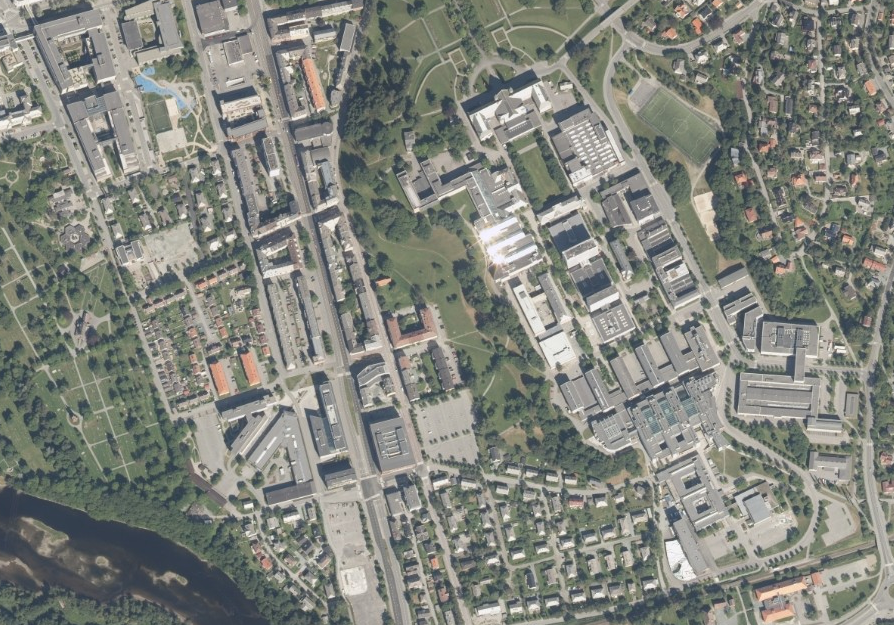
\includegraphics[width=0.8\columnwidth]{figs/aerial_image.png}
\caption[Aerial image]{An aerial image captured above NTNU.}
\label{fig:aerialimage}
\end{center}
\end{figure}

A \ac{CNN} is a special variant of a neural network, where connectivity between units have been constrained and parameter sharing is employed. This will reduce the number of parameters in the model. \ac{CNN}s can, therefore, have many hidden layers, which enables the network to learn a hierarchical representation of the input data. By having a large dataset and conducting normal back-propagation, the network can learn to extract informative features from raw pixel values. \\

This might be well suited for a road extraction system, where there are an abundance of aerial images available covering large areas. Labels can easily be generated for these areas from digital maps stored in a \ac{GIS} database. However, a large issue with utilizing aerial images for training a machine learning algorithm is the presence of noise in the labels. For most purposes maps can be created without pixel level accuracy and still retain their usefulness. The result is that datasets created from digital maps have some degree of label noise, which can have negative consequences for the accuracy achieved by a machine learning algorithm. \cite{Mnih_aerial_images_noisy} have identified two types of label noise present in aerial images: Omission and registration error. The former occurs when an object in an aerial image is missing, and the latter happens when there are a misalignment between the object in the image and in the ground truth of the label.



\section{Goals and Research Questions}
\label{sec:Goals and Research Questions}
In this section, the goal and research questions of this thesis are presented, as well as a brief motivation for each research question.

\begin{description}[ style=nextline, leftmargin=1.5em, rightmargin=1.5em]
\item[Goal statement:]{\it The goal of this thesis is to create a convolutional neural network that can extract roads from aerial images.}
\end{description}

The thesis will investigate how to further improve road extraction by considering the two research question defined below. A system consisting of a convolutional neural network will be created, and experiments will reveal how well the system performs.

\begin{description}[ style=nextline, leftmargin=1.5em, rightmargin=1.5em]
\item[Research question 1:]{\it Does the bootstrapping loss function give a significant improvement of precision and recall for datasets with noisy labels?}
\end{description}

Because of the costs involved in creating accurate datasets, the thesis will look at techniques to reduce the effect of inconsistent labelling. For datasets related to aerial images, it is common to find omission and registration error. Small and private roads are often unmarked on maps, and roads might be incorrectly placed on them.

\begin{description}[ style=nextline, leftmargin=1.5em, rightmargin=1.5em]
\item[Research question 2:]{\it How can curriculum learning improve results in deep learning, and does this improve precision and recall for aerial images?}
\end{description}

The thesis will also investigate the benefits of curriculum learning for a machine learning algorithm. By sorting examples from easy to hard, the learner can potentially be guided to a more advantageous area of parameter space and result in the learner finding a better local minimum, as well as reducing the time of convergence. This can be beneficial for deep learning, which often involves optimization of a lot of parameters. The challenge is to find ordering criteria that are applicable for aerial images. 


\section{Research Method}
\label{sec:researchMethod}
To address the research questions outlined in Section \ref{sec:Goals and Research Questions}, a \ac{CNN} has been developed. An aerial image dataset containing ground truth for roads have been acquired from \citep{MnihThesis}, and is publicly available under the name Massachusetts Roads Dataset. Additionally, a new dataset containing parts of the Norwegian road network has been created using aerial images and road centerline vectors provided by Kartverket.\\   

These datasets will be used for training and testing the performance of the system, as well as evaluating the research questions. Furthermore, by utilizing a publicly available dataset, the system presented in the thesis can be compared to the performance of other similar systems \citep{MnihThesis}\citep{saito_building_and_roads}.  

\section{Contributions}
\label{sec:IntroContributions}
{\it
The thesis' main contribution to the field of machine learning  is the examination of different approaches for reducing the impact of inconsistent labelling, and experiments conducted on semantic road labelling task which has a high rate of naturally occurring inconsistent labelling. Experiments demonstrated that curriculum learning improved the generalization accuracy of a deep neural network, trained with real-world datasets. Furthermore the thesis shows that a curriculum teacher based on inconsistency between a model prediction and a label can be effective for curriculum learning. The main contributions of this thesis are:}\todo{What about bootstrapping}

\begin{enumerate}
\item {\it Demonstrating the effectiveness of curriculum learning for real-world datasets}
\item {\it A generally applicable curriculum teacher based on ordering examples based on inconsistency between model prediction and example label}
\item {\it A new aerial image dataset covering a large area of the Norwegian road system.}
\end{enumerate}

\section{Thesis Structure}
\label{sec:thesisStructure}
The thesis is divided into five chapters. This chapter presents the motivation and research questions. In Chapter \ref{cha:TheoryAndBackground}, sections describing the background theory, the structured literature review, and related work can be found. Chapter \ref{cha:architectureAndModel} outlines the methods and implementation, as well as presenting details about the datasets. Experiment results and analysis can be found in Chapter \ref{cha:ResearchAndResults}. The final chapter, Chapter \ref{cha:evaluationAndConclusion}, concludes the thesis by summarizing the results, outlining future work and presenting the thesis' contributions.



\chapter{Background Theory and Motivation}\label{T-B}
\label{cha:TheoryAndBackground}

\section{Background Theory}
\label{sec:background_theory}
\subsection{Convolutional Neural Networks}
A \ac{CNN} is a special kind of neural network, and it was one of the first deep learning models to perform well in commercial applications. A \ac{CNN} is loosely based on principles drawn from neuroscience. According to \cite{Bengio_deep_learning_book},  local connectivity and parameter sharing are properties characteristic for \ac{CNN}s. These properties and the architecture of \ac{CNN}s will be explored further below.

\subsubsection{Convolution}
In mathematics, convolution is a mathematical operation on two real-valued functions that express the amount of overlap of one function as it is shifted over another function. For machine learning applications, the data is usually discretized. The operation is therefore a discrete summation over the data, and is used to calculate the weighted sum between the activations and the connection weights in a \ac{CNN}. The discrete convolution operation without kernel-flipping:

$$ (x*w)(t) = \sum\limits_{a=-\infty}^\infty x[a]w[t+a]$$ 

For aerial images we extend the convolution operation to two dimensions, and limit the summation to a finite number of pixels. To convolve an image I, a two-dimensional kernel K containing the weights is shifted across the image:  

$$ (I*K)[i,j] = \sum\limits_{m}\sum\limits_{n} I[i+m, j+n]K[m,n]$$ 

This operation is  visualized in figure \ref{fig:convolution} where a $2 \times 2$ kernel of weights is convolved with a $3 \times 3$ matrix of input values, and produces $2 \times 3$ outputs. 

\begin{figure}[t]
\begin{center}
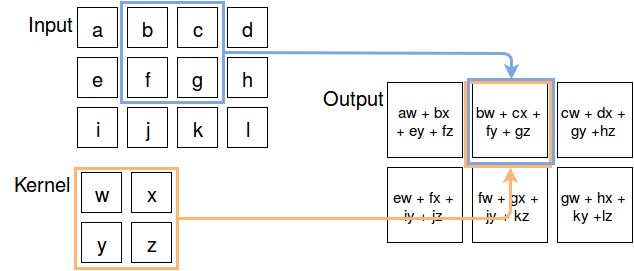
\includegraphics[width=0.8\columnwidth]{figs/convolution.png}
\caption[Convolution example]{Example of 2D convolution without kernel-flipping.}
\label{fig:convolution}
\end{center}
\end{figure}


\subsubsection{Local Connectivity}
In a traditional neural network, each layer is typically fully connected. Each unit has connections to every unit in the previous layer. In a \ac{CNN}, however, a unit interacts only with a small region of units in the previous layer. This region is often referred to as the unit's local receptive field. This kind of local connectivity can be very practical for high-dimensional data, such as images where meaningful features can be extracted using only a small area of the total image. \\

Local connectivity can be achieved by using a small kernel as seen in Figure \ref{fig:convolution}. Instead of each unit being connected to all inputs, the unit only depends on a $2 \times 2$ input region. \\

If there are $m$ inputs and $n$ units, a matrix multiplication for a fully-connected network would require $m\times n$ parameters, as well as having a runtime of $O(m\times n)$. By using a kernel we limit the number of connections each unit may have to k. This requires only $k\times n$ parameters and a runtime of $O(k\times n)$. For image applications, the kernel size can be relatively small and still achieve good results, which can give big improvements in efficiency.

\subsubsection{Parameter Sharing}
The number of model parameters is further reduced by using parameter sharing. Each weight in the kernel is applied to every position of the input. In contrast, a neural network which is fully connected will have a separate weight for every connection. This can be redundant for high-dimensional data, where most of the features are localized. In images, for example, an important feature to extract are edges. A kernel with weights that are good at detecting edges at one location, will be equally good at detecting them in other locations. \\

The use of parameter sharing further reduces the storage requirement to $k$ parameters. Usually, one kernel per layer is not enough, so several kernels with tied weights convolve the input. The layer will then produce output activations for different features. The outputs of several kernels are often referred to as feature maps.

\subsubsection{Pooling}
The pooling function is another operation typically associated with \ac{CNN}s. A pooling function modifies the output of a layer in some way. It replaces a rectangular region of the output by a single value that has been determined by a summary operation. A common pooling function is the max pooling operation, which outputs the maximum within a rectangular neighborhood. The reason for utilizing pooling is that it helps the representation become invariant to small translations in the input. For example, a network created to classify whether an image depicts a cat or not will benefit from pooling, since the location of the cat in the picture is irrelevant. For tasks where the location of a feature is important, such as semantic segmentation, applying pooling should be done with restraint. Additionally, pooling reduces the number of input parameters for the next layer.

\subsubsection{Layer Structure}
A typical convolutional layer in a network consists of three stages. First, convolution sums the weighted inputs for every unit in the layer. Second, an activation function is applied to the resulting values. The \ac{ReLU} is a popular choice, and outputs either 0 or the weighted sum, depending on which is biggest: $f(x) = max(0, x)$. Finally, the pooling function modifies the output of the layer. 

\subsubsection{Network architecture}
A \ac{CNN} usually consists of both convolutional layers and fully-connected layers. The input layer and the initial hidden layers are convolutional layers, with fully connected layers attached at the end. Figure \ref{fig:conv} shows a convolutional neural network configuration. The input layer and the two first hidden layers are convolutional layers. During training, the kernel weights for these layers are adjusted by backpropagation. Each feature map defines a set of kernel weights that are applied to all input pixels or activations. Usually, a \ac{CNN} will reduce the necessity of feature engineering because it learns what suitable features to extract from input data. In images, a \ac{CNN} is able to learn from raw pixel values without the use of feature extraction techniques found in computer vision.


\begin{figure}[t]
\begin{center}
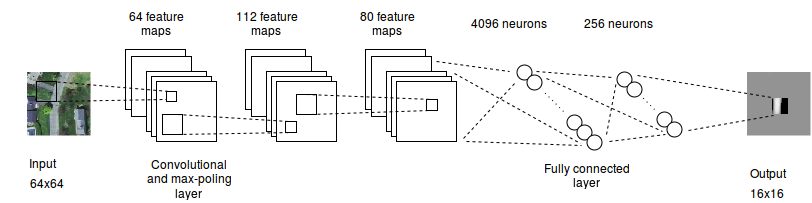
\includegraphics[width=1\columnwidth]{figs/conv_diagram.png}
\caption[Convolutional neural network]{Convolutional neural network. }
\label{fig:conv}
\end{center}
\end{figure}
\label{sec:convolutional_networks_background}

\subsection{Label Noise}
\label{sec:background_label_noise}
There are several reasons for the presence of inconsistent labels in real-world datasets. For instance, the labeller was presented with insufficient information, or the dataset was automatically generated from a source with poor quality labels. Additionally, the samples could be ambiguous and therefore hard to label correctly by a human expert. Label noise, can in many cases, lead to negative consequences for a classifier. This can include reduced accuracy, increased model complexity, and more samples required for learning a target concept. Approaches for dealing with noisy labels can generally be divided into three groups: Data cleansing methods, noise-robust models, and noise-tolerant algorithms \citep{Frenay_label_noise_survey}. These three groups are presented below.  \\

%\subsubsection{Types of noisy labels}
%Based on the noise distribution, three types of label noise can be identified according a extensive survey on label noise by \citep{Frenay_label_noise_survey}. The different types can be viewed in Figure ??\todo{Figur}. X is a vector of features or the data. For all types the observed variable Y* is assumed to depend the true label Y.  The E is a binary variable indicating if an labelling error has occurred. 

%Noisy completely at random (NCAR) model.

%Noisy at random (NAR) model. 

%Noisy not at random (NNAR) model


\subsubsection{Data Cleansing Methods}

Data cleansing methods are filtering techniques applied to the training data in order to remove noisy samples before training. Noisy labels are first identified and then either relabelled or removed. An obstacle encountered by these methods is that harmful mislabelled samples can be difficult to distinguish from informative, but hard samples. Another problem is that filtering often relies on classifier predictions to automatically identify mislabelled samples. Such filtering techniques also run the risk of removing too many samples from the training set, which can also cause harm to the accuracy. Voting ensembles of several classifiers have been suggested to further improve classification filtering.\\ 

Another filtering technique is to simply remove the class label of samples deemed suspicious, and employ semi-supervised learning. This way, the distribution of samples are preserved while simultaneously reducing the consequences of inconsistent labels.\\


\subsubsection{Noise-robust Models}
Noise-robust models are algorithms that are naturally robust against label noise. Many algorithms have been shown to be less sensitive to label noise than others, especially to small amounts of label noise. This approach requires no noise modelling nor cleansing of the training set beforehand, because the algorithm is assumed to offer some robustness to mislabelled samples.\\

 Algorithms that utilize regularization techniques to avoid overfitting, can be considered more robust to label noise. This can include convolutional networks that utilize regularization schemes such as dropout or weight decay. For ensemble methods, bagging often gives better results than boosting when faced with noisy labels \citep{Dietterich_boosting_bagging}. The boosting algorithm AdaBoost, for example, combines many weak classifiers by iteratively re-weighting the training set to target samples the previous classifier had trouble predicting. Because mislabelled samples can be harder to predict, AdaBoost tends to put larger emphasis on mislabelled samples in later stages of learning, which can lead to increased sensitivity to label noise. In bagging methods, however, different subsets of the training data are used to create a diverse set of classifiers that are employed in a voting scheme. In this case, mislabelled samples can impact the performance positively, due to the increased variability in the classifiers.   


\subsubsection{Noise-tolerant Algorithms}
In noise-tolerant approaches, existing algorithms are modified to be more robust towards label noise. This is often done by explicitly modelling a noise model during training. This way, a classifier learns to classify samples according to their true uncorrupted label, instead of the observed noisy label. Typically, the noise distribution and the model parameters are estimated simultaneously when training the classifier. \\

Techniques that incorporate label noise tolerance, such as particle competition, noise model estimation, bootstrapping, and co-training, will be further discussed in Section \ref{sec:related_works}.

\subsection{Curriculum Learning}
Curriculum learning is inspired by how humans learn, and that learning typically is highly organized. For instance, by the use of a curriculum in educational institutions. Easier concepts tend to be introduced first. In terms of machine learning, this means presenting the classifier with easier samples first while training. To do so, a curriculum strategy has to be defined, which sorts the training set from easy to hard. Samples that are not near the decision boundary could be considered easy, for instance. Utilizing curriculum learning might lead to a faster convergence time, and the algorithm reaching a better local minimum. Different works show that curriculum learning can achieve better generalization for many tasks \citep{Bengio_curriculumlearning} \citep{Kumar_self_paced_learning} \citep{Lu_self-paced_learning_diversity}.\\

A challenge for curriculum learning is defining a sorting measure that enables a curriculum strategy of gradually introducing harder training samples to the learner. This issue, and works related to curriculum learning, is further explored in Section \ref{sec:related_works}.\\

\subsection{Road Extraction by Machine Learning}
Road extraction is a part of the field of Photogrammetry, and involves technology for map production and measurements of objects in images. As digital acquisition systems for capturing aerial images have become commonplace, the availability of high-resolution aerial images have increased. Coupled with the increasing need for detailed spatial information in \ac{GIS} databases and production of digital maps, a lot of approaches for automatic object extraction from aerial imagery have been suggested. A reliable and accurate detection system could be beneficial in terms of increased levels of details, while reducing the cost associated with map production.\\

There are three distinctive approaches for extracting objects from aerial imagery. Manual, semi-automatic and automatic methods. The semi-automatic approach integrates computer vision techniques and machine learning into the workflow of skilled human labellers. For instance, Google's Ground Truth project employs skilled operators which utilize advanced software tools to improve the accuracy of Google's map products \citep{Ground_truth}.\\

To do automatic road detection, supervised learning is often employed. This requires a training dataset of aerial images and labels. The labels for road detection are usually binary images that show the ground truth of roads. Creating the label images by manually labelling aerial imagery would be prohibitively expensive, which is why ground truth labels are often generated from existing map data. Figure \ref{fig:background_dataset_example} shows an example of an aerial image and a label typically found in a road segmentation dataset.\\

\begin{figure}
\begin{subfigure}{0.40\textwidth}
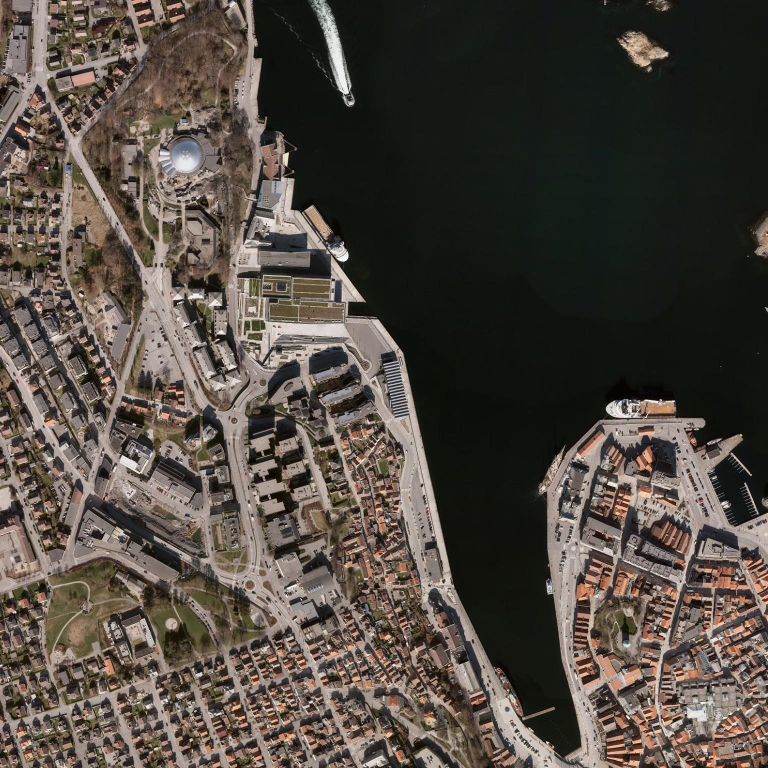
\includegraphics[width=\linewidth]{figs/background_theory_example_data.png}
\caption{Aerial image} \label{fig:background_dataset_example_data}
\end{subfigure}
\hspace*{\fill} % separation between the subfigures
\begin{subfigure}{0.40\textwidth}
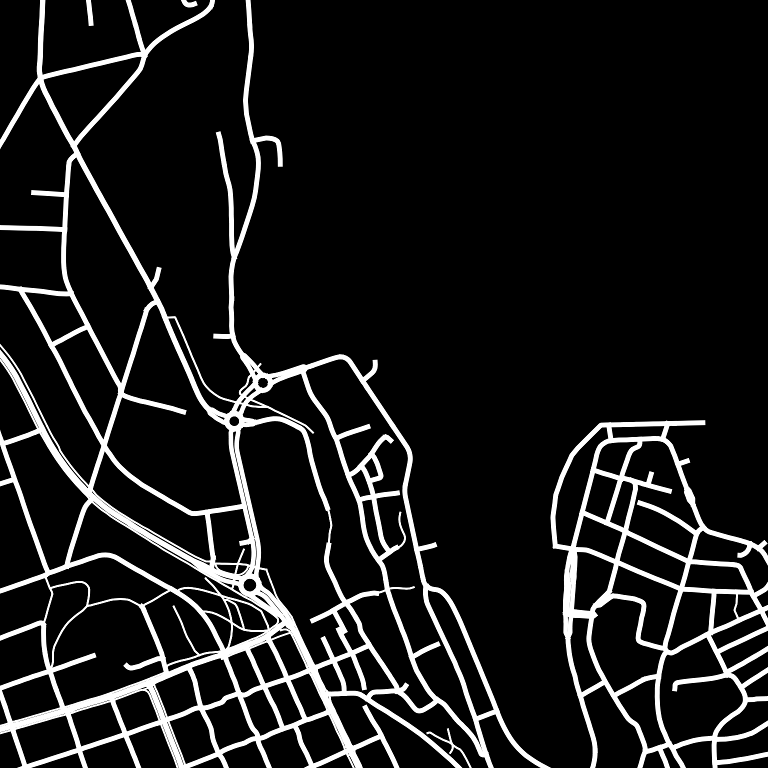
\includegraphics[width=\linewidth]{figs/background_theory_example_label.png}
\caption{Label image} \label{fig:background_dataset_example_label}
\end{subfigure}
\caption[Example from the Norwegian Roads Dataset]{Image and label example from the training set of the Norwegian Roads Dataset.} \label{fig:background_dataset_example}
\end{figure}

From these large training set images, smaller training set patches are extracted. The supervised learning algorithm is given a patch dataset $d$ containing $N$ training examples in the form $d=\{(s_1, m_1),...,(s_N, m_N)\}$, where $s_i$ is an aerial image patch and $m_i$ is the corresponding ground truth label. Examples of aerial image patches and labels can be found in Figure \ref{fig:examples_background}. The learning algorithm's task is to learn a suitable mapping from the input space of aerial imagery to the output space of road ground truth. In neural networks, this mapping is typically learned by minimizing the cross-entropy loss by gradient descent optimization.\\

\begin{figure}
\begin{center}
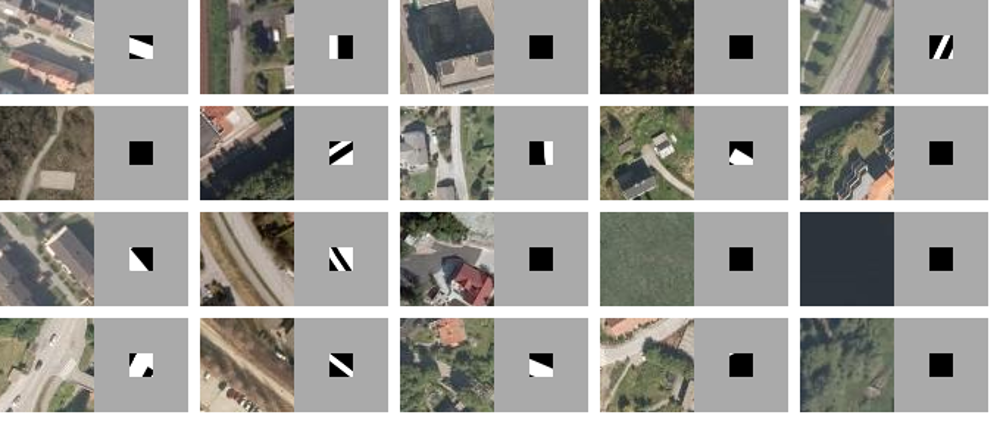
\includegraphics[width=1\columnwidth]{figs/examples.png}
\caption[Patch dataset examples]{Aerial image and label examples from a patch dataset. The patches originate from the Norwegian Roads Dataset. Each label depicts the road ground truth from the center location of the aerial patch.}
\label{fig:examples_background}
\end{center}
\end{figure}

 The resulting classifier has hopefully extracted some useful patterns from the training data, which enables it to generalize to the task of road extraction. This is verified by computing the \ac{MSE} on a test set, containing examples not seen during training. The machine learning approach for road extraction should therefore be able to train algorithms from data which can predict the ground truth reasonable well for new unseen aerial image patches. \\

\subsection{Evaluation Metrics}
A common way to evaluate road extraction systems is by the quality measures,  correctness and completeness \citep{Wiedemann_road_evaluation}. These are closely related to precision and recall. Precision measures the fraction of true roads that are correctly detected, while recall is the fraction of predicted roads that are true roads. Because the label maps are not perfectly aligned with the images, it is also common to use a relaxed measure of precision and recall. This is accomplished by treating predicted road pixels within $p$ pixels of a true road pixel as being correctly detected. True roads within $p$ pixels of a predicted road pixel are considered correctly recalled. The slack parameter $p$ is often set to 3 pixels \citep{Mnih_roads_high_res_aerial_images}.



\section{Structured Literature Review}
\label{sec:slr}
The purpose of conducting a \ac{SLR} is to get an overview of the field of remote image sensing, as well as the research related to curriculum learning and dealing with noisy labels. The \ac{SLR} method has been chosen to investigate these topics, and provides a formal way of identifying the information available.

\subsection{Identification of Research}
This section outlines the strategy that was utilized to search for primary studies. By utilizing a search strategy, literature relevant to the defined research questions can be identified and collected. Search terms have been defined, as well as literature resources.

\subsubsection{Literature Resources}
\label{sec:literature_resources}
The following resources was searched in order to identify and collect relevant material:
\begin{itemize}
	\item ACM digital library
	\item IEEExplore
	\item ScienceDirect
	\item CiteSeer
	\item Springer Link
	\item ECCV (conference)
	\item NIPS (conference)
\end{itemize}

\subsubsection{Key Terms and Groupings}
Table \ref{tab:search_terms} describes the different word groups employed by the search strategy. Each group specifies a number of terms that are either synonyms or related to each other. Additional terms have been appended, as a result of a search strategy validation.


\begin{table}[htp]

\caption[The terms and groups]{The terms and groups.}
\begin{center}
\begin{adjustbox}{max width=\textwidth}
\begin{tabular}{+c | ^p{0.12\textwidth} ^p{0.14\textwidth} ^p{0.15\textwidth} ^p{0.19\textwidth} ^p{0.15\textwidth} ^p{0.12\textwidth} }\hline
\rowstyle{\bfseries}
 		& Group 1 & Group 2 & Group 3 & Group 4 & Group 5 & Group 6\\\hline
\textbf{T1} 	& Aerial images & Curriculum learning & Noisy labels & Neural network & Segmentation & Roads\\
\textbf{T2}	& Satellite images & Guided learning & Missing \mbox{labels} & Convolutional neural network & Classification & \\
\textbf{T3} 	& Remote sensing & Example ordering & Semi-supervised & Machine \mbox{learning} & & \\
\textbf{T4} 	& Images & & Noisy data (appended) & Deep \mbox{neural} networks (appended) & & \\\hline
\end{tabular}
\end{adjustbox}
\end{center}
\label{tab:search_terms}
\end{table}

\subsubsection{Search Strategy}
Based on Table \ref{tab:search_terms} several search expressions were devised. Each of these expressions were run for each of the resources listed in the literature resources section. 

\begin{itemize}
	\item (aerial images OR satellite images) AND (segmentation OR classification)
	\item (remote sensing OR aerial images) AND (noisy labels OR missing labels OR semi-supervised OR noisy data)
	\item (neural network OR machine learning OR convolutional neural networks) AND (aerial images OR satellite images)
	\item (curriculum learning OR guided learning) AND (machine learning OR neural networks OR deep neural networks OR  convolutional neural network) 
	\item (segmentation OR classification) AND (roads)
	\item (Noisy labels OR missing labels OR semi-supervised OR noisy data) AND (machine learning OR neural network OR convolutional neural network)
	\item (aerial) AND (noisy labels OR missing labels OR semi-supervised OR noisy data) AND roads
\end{itemize}

\subsection{Selection Process}
The search expressions resulted in a large number of hits for each resource. The top 15 results for each expression were stored, and a  selection process was created to reduce the over 400 studies to a more manageable number. At first, the title of each study was evaluated. If the title seemed unrelated to the research goal or the research questions found in Section \ref{sec:Goals and Research Questions}
the study was removed. Then the title and the abstract were evaluated using the inclusion criteria defined in Table \ref{tab:selection_critera}. Finally, the remaining studies were read while considering both the inclusion and quality criteria.

\begin{table}[htp]
\caption[Inclusion and quality criteria for the selection process]{Inclusion and quality criteria for the selection process.}
\begin{center}
\begin{adjustbox}{max width=\textwidth}
\begin{tabular}{+l ^p{8cm} ^r}\hline
\rowstyle{\bfseries}
Id & Criteria & Screening step\\\hline

IC 1 & The study's main concern is curriculum learning, dealing with noisy labels or road extraction systems  & 1\\
IC 2 & The study is presenting empirical results & 1\\
IC 3 & The study preferably involve machine learning & 1\\
QC 1 & The research has a clear aim & 2\\
QC 2 & Is there an adequate description of related works? & 2\\
QC 3 & How rigorously has the method or technique been tested? & 2\\
QC 4 & Is there a future work section?
 & 2\\\hline
\end{tabular}
\end{adjustbox}
\end{center}
\label{tab:selection_critera}
\end{table}

\subsection{Other Resources}
By conducting a \ac{SLR}, a number of relevant studies were identified. Additional literature was discovered by finding works citing the \ac{SLR} papers on Google Scholar, and reading survey papers on road extraction systems \citep{Mena_GIS_state_of_the_art} \citep{Trinder_towards_automation} and label noise \citep{Frenay_label_noise_survey}. The surveys provided a comprehensive overview of these topics and enabled further identification of relevant literature.

\section{Related work}
\label{sec:related_works}
\subsection{Road Extraction Systems}
There is a large amount of literature regarding proposed methods for automatic road extraction systems. This includes segmentation, edge detection, knowledge based methods, fuzzy classification methods, and region growing methods. For a thorough review of different road extraction systems, see \citep{Trinder_towards_automation}
\citep{Mena_GIS_state_of_the_art}. The main aim of this section is to present approaches based on machine learning.

\subsubsection{Types of Aerial Imagery}
Aerial and satellite imagery are captured using a whole range of sensors. A lot of approaches found in remote sensing are developed for certain types of sensor data. Below is a list of different types of aerial imagery:
\begin{itemize}
 \item Monochromatic (single channel or greyscale) images 
 \item Infrared band
 \item Color images (Red, green and blue channel)
 \item Hyper-spectral images
 \item Synthetic aperture radar images (SAR)
 \item Laser images (LIDAR)
 \end{itemize}

The focus of this review is approaches for color images, which is the most common type of aerial imagery.

\subsubsection{Machine Learning}
In the previous two decades, the availability of high resolution images covering large areas have increased. These images can have a resolution of around 1 square meter per pixel or higher. At this resolution, finer details such as cars, buildings and trees can be distinguished. Having a higher resolution for images also result in much more variability in terms of shape, texture and illumination. Machine learning algorithms that can learn highly non-linear decision boundaries have therefore become more common for aerial imagery applications. To successfully discriminate between object classes, more spatial context have been used to create a richer feature representation, as well as more data being used for training. Additionally, structured prediction methods such as \ac{CRF}, have become popular for smoothing in semantic segmentation applications.


\subsubsection{Classifiers}
High-resolution aerial imagery has created a need for more sophisticated classifiers. A classifier must encode knowledge of shape and context in order to discriminate between similar objects. In a road extraction system for high resolution imagery, the classifier should, for example, be able to distinguish between roads and grey rooftops. The classifier is therefore required to learn highly non-linear decision boundaries. This can include \ac{SVM}, ensemble methods and deep neural networks.\\

In \cite{Mayer_road_test} six road extraction approaches were compared on both aerial images and satellite images. The approaches were based on image processing techniques, especially line detection. Many of the approaches rely on characteristics specific to roads, such as identifying parallel lines in images. In addition, some approaches utilized fuzzy classification or unsupervised clustering. Both scenes from urban and rural areas were used for the comparison. The authors defined a minimum of 0.6 and 0.75 in precision and recall, in order for a raod extraction system to be of any practical use. In summary, most of the approaches performed well for images with limited complexity, such as rural areas. None of the methods performed above the defined threshold for images containing suburban or urban scenes. The low performance for urban areas reinforces the need for classifiers that can learn complex decision boundaries.\\

A hybrid approach for road extraction using \ac{SVM} and image processing techniques was proposed by \cite{Song_road_extraction_svm}. First, a \ac{SVM} classifies images into a road and a non-road set. Second, the images in the road set are segmented into homogeneous areas by utilizing the region growing technique. \\

The \ac{SVM} did not perform sufficiently well for areas that appear similar to roads, especially for urban areas, with structures such as parking areas and roof tops. Therefore, they extract shape descriptions from the segmented regions, and exploit road characteristics to remove areas not corresponding to roads. This is done by a threshold operation on shape descriptions such as smoothness and density.\\

 The approach was tested experimentally on IKONOS satellite images. The approach performed well. However, road segments obscured by shadows or overhanging trees were a problem, as well as narrow roads and intersections.\\

Ensemble methods have also been applied to tasks involving aerial imagery. In \citep{Kluckner_semantic_height}, randomized forest was used for land cover classification on high-resolution imagery. Training a randomized forest involves training several binary decision trees on subsets of the training data. The result is an ensemble of weak classifiers that together can provide robust and accurate predictions. \cite{Dollar_supervised_edge} proposed a supervised edge detection method, which was tested for road detection. This method trains a boosted tree classifier, which is similar to a decision tree, except that boosted classifiers are used to split the data at each node in the tree.\\

\cite{Mnih_roads_high_res_aerial_images} proposed an automatic road extraction approach for large real-world datasets. The system consists of a neural network with millions of weights that is trained on a large dataset of aerial images. A \ac{GPU} was utilized to train the network.  \\

They formulated detection of road pixels from aerial images as a patch-based semantic segmentation problem. 
The goal of the model is to predict whether or not pixels belong to a road class, given an image patch. This is achieved by having the neural network model the distribution:

 $$p(N(M(i,j), w_m) \mid N(S(i,j), w_s),$$ 
 
\noindent where $S$ is an aerial image and $M$ is a corresponding road label image. $M(i,j) = 1$ if $S(i,j)$ is a road pixel and 0 otherwise.  $N(I(i,j), w)$  denotes a $w \times w$ large patch of pixels centered at location (i,j) of a large image $I$. Using smaller image patches instead of entire images for modelling the distribution, limits the image context which the model use to make predictions. This approach is less computational expensive, and by retaining a relatively large $w_s \times w_s$ can still provide enough image context to create a competent road detector. \\

The network consisted of a single hidden layer with 12288 units, an input layer of 4096 units, and 256 output units. This enables the network to predict 16 x 16 road prediction patches given 64 x 64 aerial image patches. The network was trained by \ac{SGD} to minimize cross-entropy between training labels and the predicted map patches. Furthermore, unsupervised pre-training was used to initialize the parameters of the network.\\

Experiments have been conducted on two large aerial image datasets, and the network achieved good performance both in terms of precision and recall. A problem identified by \cite{Mnih_roads_high_res_aerial_images}, is that the model is penalized for correct predictions because of noisy labels. Smaller roads or paved areas have often not been marked in the dataset. Additionally, the road labels in the dataset have been generated from road center-line vectors with a fixed width, which results in some roads not being covered by the ground truth. This may lead to a decrease in model performance, since the model is penalized for correctly labelling the roads when minimizing the cross-entropy between predictions and inconsistent labels.\\

The problem with inconsistent labels in the context of aerial images was investigated in \citep{Mnih_aerial_images_noisy}. Two loss functions were proposed to deal with label noise found in aerial imagery. This model resembles the patch-based approach used in \cite{Mnih_roads_high_res_aerial_images}. However, a deep neural network consisting of three hidden layers was used. The first two hidden layers are locally connected layers, while the final hidden layer is fully connected. Unlike convolutional neural networks, there are no parameter sharing involved. \\

The proposed deep neural network performed significantly better in terms of precision and recall, compared to the shallow neural network in \citep{Mnih_roads_high_res_aerial_images}. By utilizing the robust loss functions, performance was further improved.\\

In addition, convolutional neural networks have been trained to do road detection. Both \cite{MnihThesis} and \cite{saito_building_and_roads} have tested this type of network, on the publicly available datasets, Massachusetts Roads Dataset and Massachusetts Buildings Dataset. The networks consisted of 5 layers, three convolutional layers and two fully connected layers. The networks utilized stride and max-pooling, but only in the first layer. They did however chose different kernel sizes for the convolutional layers. For instance, the \citep{MnihThesis} used a first layer kernel size of $16 \times 16$, whereas \cite{saito_building_and_roads} used a kernel size of $9 \times9$.  Both dataset was trained on patches of $64 \times 64$ pixels. However, \cite{saito_building_and_roads} extended the detection task to simultaneously prediction road and building footprint pixels, by training the network on a merged version of the previously mentioned datasets. Predictions were made by an output layer of 768 units, which represent a three channel $16 \times 16$ prediction patch. Each prediction patch pixel indicates by three probability values whether an input pixel belongs to the non-road, road and building class.\\

\subsubsection{Larger Datasets}
Learning complex decision boundaries and the variations present in the high-resolution aerial imagery requires a lot of training data. In previous studies, much smaller datasets have been used \citep{Mokhtarzade_road_ann} \citep{Song_road_extraction_svm}. Only eight test images ranging from 1600 to 4000 pixels in width and height were utilized to evaluate automatic road extraction approaches in \citep{Mayer_road_test}. The trend in road extraction and land cover classification literature is to use increasingly larger datasets.\\

A high-resolution aerial dataset used to optimize the randomized forest algorithm in \citep{Kluckner_semantic_height}, contains  155 images and covers an area of about 85 square kilometers. Each of these images are 11500 x 7500 pixels in size and have a \ac{GSD} of 8 centimeter.\\

In both \citep{Mnih_roads_high_res_aerial_images} and \citep{Mnih_aerial_images_noisy}, two large datasets were used to optimize neural networks with many parameters. These datasets covers 500 square kilometers at \ac{GSD} of around 1.20 meters per pixel.\\

The Massachusetts Roads Dataset introduced by \cite{MnihThesis}, consist of 1171 aerial images, each with a height and width of 1500 pixels. The dataset covers an area of over 2600 square kilometers, and contains a variety of regions, such as urban, suburban and rural areas. The \ac{GSD} is 1 meter per pixel.\\


\subsubsection{Feature Representation}
Another trend in road detection is to extract features from larger contexts or pixel neighbourhoods. In addition to increasing the classifiers ability to discriminate between objects sharing similar texture and shape, using larger contexts are necessary for images with a low ground sampling distance.\\

\cite{Mokhtarzade_road_ann} proposed using a shallow neural network for road detection. For this approach, a normalized $3 \times 3$ neighbourhood of pixel values was used as input features to a neural network. The neural network is illustrated in Figure \ref{fig:zoej_neural_network}. \\

\begin{figure}
\begin{center}
\includegraphics[width=.6\columnwidth]{figs/zoej.png}
\caption[Shallow neural network]{Pixel neighbourhood and shallow neural network used for road detection by \cite{Mokhtarzade_road_ann} }
\label{fig:zoej_neural_network}
\end{center}
\end{figure}

In \cite{Song_road_extraction_svm}, shape description is generated from segmented images, and certain characteristics descriptive of roads, such as being lengthy and narrow, are used to remove objects that share spectral similarities with roads. Each shape's border length, area, pixel count and approximate radius are used for measuring the shape index and density. Road shapes should have a large shape index value and a small density. Questionable shapes with measurements not characteristic of roads are removed by a threshold operation.\\

A much larger neighbourhood of pixels were utilized as features in \citep{Mnih_aerial_images_noisy} and \citep{Mnih_roads_high_res_aerial_images}. In this case, $64 \times 64$ pixels with minimal pre-processing formed the input to both  networks. Furthermore, the neural network learns suitable features which enables it to distinguish road pixels from non-road pixels. The large neighbourhood is helpful when resolving ambiguities often found in suburban environments, such as flat grey roof-top and roads. \\

  Combining images with height or elevation information can also increase classifier accuracy. For instance, height information makes grey rooftops easier to distinguish from street areas. The effectiveness of combining images and height maps was demonstrated by \cite{Kluckner_semantic_height} where both color and height cues were integrated as features. The height information significantly improved the performance of the classifier.
  

\subsubsection{Conditional Random Fields}
The smoothness assumption is a strong piece of prior knowledge we have about images. Neighbouring pixels tend to influence each other, and are more likely to belong to the same object or class. \ac{CRF} is a way to explicitly model dependencies between neighbouring pixels, and is often utilized in semantic segmentation tasks to obtain a smoother segmentation result. The goal of semantic segmentation is to split an image into disjoint regions, where each region is associated with a certain class label.\\

In the study by \cite{Kluckner_semantic_height}, an approach for land cover classification given high resolution aerial images was presented. Aerial images were segmented according to five classes: Building, tree, waterbody, green area, and streetlayer. Attributes such as color and edge response were extracted from aerial images, and combined with height information to create an efficient feature representation based on covariance matrices. A randomized forest classifier was trained to learn a conditional probability distribution over the possible class labels given the feature representation. The \ac{CRF} approach was tested in combination with this classifier, and was shown to significantly improve accuracy for semantic segmentation tasks. \\ 

Normally, a classifier predicts each label independently. However, for structured prediction tasks, such as segmentation, contextual information can be useful. The \ac{CRF} approach combines graphical modelling and classification. It involves minimizing the cost of a label assignment for a pixel, as well as the cost of this assignment in relation to the neighbouring pixel assignments. The cost of a label assignment, which is called the unary potential can be estimated from a prediction made by a classifier. The neighbourhood cost is calculated through the pairwise class potentials between the input and it's neighbours.\\

\ac{CRF} is often formulated as a graph with $V$ nodes, where each node represents a pixel, and can be assigned a label $l$ from a discrete set of classes, such as grass, tree, roads. The edges are represented by the set $E$, and models the relationship between neighbouring pixels or nodes. The energy of a label assignment is modelled by:

$$E(y) = \sum\limits_{i\in V} \Psi_i(l_i, x_i) + \sum\limits_{i,j\in E}\Psi_{ij}(l_i, l_j),$$

where $\Psi_i(l_i, x_i)$ is the unary potential modelling the likelihood of pixel x having a label assignment $l$. These estimates can be obtained from a classifier.  $\Psi_{ij}(l_i, l_j)$ is the pairwise potential modelling the coherence of neighbouring pixels. The final label assignment $\hat{y}$, which takes the label assignments of neighbouring pixels into account, is obtained by minimizing the energy:  $\hat{y} =argmin_y E(y)$. Whereas the first term of $E(y)$ prefers the label assignment with the lowest cost, the pairwise potentials prefer pixel neighbourhoods to have similar label assignments. This results in the most probable label assignment $\hat{y}$ given the neighbourhood.\\

\ac{CRF} is also commonly used for semantic segmentation tasks involving general scene understanding. \cite{LeCun_semantic} investigated road scene understanding by utilizing semantic segmentation for imagery found in environments encountered by vehicles. In this approach, a \ac{CNN} is trained to extract features and predict image patches. These class predictions are in turn utilized by the \ac{CRF} as unary potentials.\\

The proposed method was tested on Cambridge-driving Labelled Video Database, which contains high resolution images of roads, signs, pedestrians and other objects found in a driving vehicle environment. The use of \ac{CRF} did improve the overall accuracy, especially for large classes such as roads. For classes with less presence in the dataset the accuracy decreased.\\

Improvements in classification accuracy is further shown empirically by \cite{Schindler_random_field_overview}. Several random field techniques were tested on different aerial image datasets with low ground sampling distance. Enforcing a smoothness prior significantly improved accuracy. \\

An approach similar to \ac{CRF} is proposed by \cite{Mnih_roads_high_res_aerial_images}, where a post-processing step is introduced to improve the predictions produced by the neural network by incorporating knowledge about nearby predictions. This is achieved by training another neural network that predicts 16 by 16 map patches using 64 by 64 patches of predictions. The approach was applied to reduce the amount of gaps and disconnected road present in the baseline predictions. 

\subsection{Dealing with Noisy Labels}
Supervised learning works well for applications where there are a lot of labelled data available. For object recognition, the large-scale image database ImageNet have often been utilized. This database provide millions of manually annotated and quality controlled images, organized in a semantic hierarchy \citep{Deng_imagenet}. However, for some tasks, such as semantic segmentation and object detection, manually labelled data are expensive and time consuming to create, and high quality datasets can be hard to obtain. Automatically creating large dataset from internet resources, such as image search engines, \ac{GIS} databases, and user annotated images can be very practical in terms of reducing the costs of creating very large datasets. \\

Unfortunately, such datasets will often contain noisy or weak labels. User annotation for images are usually incomplete, image search engines often return images unrelated to the search term, and \ac{GIS} databases might be outdated and missing important object information. This can have negative consequences for a supervised algorithm, which in most cases assume that the labels are correct. These consequences are more evident in datasets containing substantial amount of inconsistent labels.\\
 
There are three main approaches to dealing with noisy label, as outlined in Section \ref{sec:background_theory}. However, in this section only noise-tolerant algorithms are explored, and especially methods that explicitly introduce noise tolerance into deep neural networks.  

%\subsubsection{Modelling the noise distribution}
%Compare the different approaches for modelling the noise.

\subsubsection{Learning to Label Aerial Images from Noisy Data}
The problem with inconsistent labels in aerial images was investigated in \citep{Mnih_aerial_images_noisy}. In this work, two types of label noise were identified,  which datasets constructed from maps are especially susceptible to. Omission noise is defined as objects that appear in the aerial image, but not in the map. Registration noise occurs when the location of the object in the map is inaccurate. Considering that the presence of label noise might negatively impact the classifier accuracy, \cite{Mnih_aerial_images_noisy} proposed two robust loss functions that can be incorporated in a deep learning framework. \\

The first loss function proposed explicitly models asymmetric noise, and is designed to deal with omission noise. It treats label $\tilde{y}$ as a noisy observation generated from true label $y$, according to a noise distribution $p(\tilde{y} \mid y)$. This distribution is determined by two parameters, set before training. The noise model modifies the derivatives produced by the loss function, which results in the neural network being penalized less for making confident, but incorrect predictions. \\

The second loss function is an extension of the first, and considers both omission and registration error. The noise distribution model combines with a generative model, where different crops of an unobserved, perfectly registered map are generated. These crops are used by an expectation–maximization like algorithm to estimate the true label, which can reduce the effect of local registration errors.\\


The loss functions were evaluated on two large aerial road detection datasets. There was a significant improvement in precision and recall for both loss functions, compared to the baseline deep neural network and the network in \citep{Mnih_roads_high_res_aerial_images}. The second loss function performed slightly better than the first for one of the datasets. This dataset had substantial amounts of registration errors.\\


\subsubsection{Training Convolutional Networks with Noisy Labels}
\cite{Sukhbaatar_noisy_network_learning} demonstrate robustness towards label noise in a modified \ac{CNN}. The method models the noise through an additional noise layer which is estimated alongside the network parameters during \ac{SGD} training. The combined model is optimized to predict the noisy labels. The goal of the noise layer is to approximate the noise distribution of the data and thereby forcing the base model to predict the true labels. Experiments were conducted for several datasets, and showed that the approach does well for higher levels of label noise. \\

Like other noise-tolerant methods, the algorithm involves learning a noise distribution, where the examples observed by the algorithm have been altered by a noisy distribution. The noise distribution is parameterized by a matrix Q, where each value specifies the probability of observing noisy label $\tilde{y}$ given the true label $y$: $q_{ji} := p(\tilde{y} = j \mid y = i)$. \\

The matrix Q is implemented by a constrained linear noise layer, which is added to the base model. This is illustrated in Figure \ref{fig:fergus_method}. The weights between the output layer of the base model and the noise layer corresponds to probabilities found in Q. These conditional probabilities $q_{ji}$ are usually unknown, but an approximate noise distribution can be estimated by conventional back-propagation. \\

\begin{figure}
\begin{center}
\includegraphics[width=.6\columnwidth]{figs/Fergusmethod.png}
\caption[Noise matrix Q]{Noise matrix Q is inserted between loss function and output layer of the model.}
\label{fig:fergus_method}
\end{center}
\end{figure}

The training procedure starts with Q fixed to the identify matrix, while the base model is trained. After a number of epochs, the weights in the linear noise layer will also be adapted by back-propagation. To ensure that Q captures the noise properties of the data, a regularization term is used to make it converge to the true noise distribution. Effectively, the prediction of the combined model will be given by:

%Is a regularization term used, or regularizer?
$$p(\tilde{y} = j \mid x) = \sum_{i} q_{ji}p(y = i \mid x),$$ 

where the noisy predictions are made by the conditional probabilities encoded in q and the prediction of the base model. Hopefully, the base model will learn to predict the true labels $y$ instead of the noisy labels $\tilde{y}$.  \\

The approach was tested using the Google street-view house number, CIFAR10 and ImageNet dataset. Noisy labels were synthesized by switching labels of examples with a fixed probability defined by a probability matrix. \\

The noise layer extension consistently achieved better accuracy compared to the baseline network, and also displayed more robustness to inconsistent labelling. Furthermore, the performance of the modified network decreased slower with increasing noise levels. This approach was also efficient in learning the noise distribution. \\

For the ImageNet dataset, the labels were switched on half of the examples in the dataset. The approach did better than the baseline model. Additionally, the approach also outperformed the baseline model trained on the clean unaltered subset of the dataset, showing that the noisy examples carry useful information.


\subsubsection{Training Deep Neural networks on Noisy Labels with Bootstrapping}
In \cite{Reed_noisy_labels_bootstrapping}, a generic approach to handling noisy and incomplete labels in supervised deep learning was presented. The approach incorporate a notion of perceptual consistency in the loss function. A prediction is consistent if the same prediction is made given similar percepts. The learner is allowed to disagree with inconsistent labels by using its own implicit knowledge stored in the network parameters.\\ 

They present two ways of incorporating perceptual consistency in a network. The first involves a reconstruction loss and a noise distribution model. The other method is introduced as bootstrapping, and avoids directly modelling the noise distribution, by using a combination of training labels and the current model's prediction to generate targets.\\

The bootstrapping approach tweaks the loss function to be a convex combination of the model prediction $q$ and the label $y$. The $\beta$ parameter decides the prediction's contribution to the convex combination, and is usually set to a relatively low value. The bootstrapping loss function is denoted:

$$\mathcal{L}(q,y) = - \sum\limits_{k=1}^L [\beta y_k + (1-\beta)z_k]log(q_k),$$

where $z_k$ is assigned a value of 1 for the most probable class $q_i$, given the data. \\

This approach was tested on several image tasks, and yielded substantial improvements for several datasets. For all tasks, deep neural networks were trained and used as the baseline. The networks that were modified to include perceptual consistency were trained by fine-tuning the baseline parameters. \\

The developed method performed better than the baseline. For MNIST handwritten digits dataset, artificially label noise was added. The bootstrapping performed significantly better than the baseline for noise fraction above 35 percent.\\

In the task of emotion recognition using Toronto Faces Database, bootstrapping performed better than the baseline and other approaches. This dataset contains over 4000 face images with emotion labels. This kind of labelling can be subjective and the dataset might therefore contain mislabelled samples. \\

Overall, bootstrapping improves the robustness of a model and is fairly simple to implement. The bootstrapping approach achieves comparable performance to loss functions that require a noise distribution model. Further improvements could be achieved by learning a time-dependent $\beta$ for the loss function.


%-So introducing another softmax layer. Model true class labels oppsed to label observations. Weights between output layer and this new layer should learn the log-probabilities of observing true label j as noisy label k. Doing gradient ascent logP(t|x)  does not do anything yet, because no explicit incentive for te model to treat q as true label. Structure of RMB, t and x conditionally independent given .


%Model trained with a generative objective. Approximate gradient ascent logP(x,t), contrastive divergence. Generative training provides notion of consistency between x and prediction q.

%Feed forward version as follows. Trainable via gradient descent, autoencoder version. :

%$L_{recon}(x,t) = - \sum\limits_{k=1}^L log P(t_k =1 | x) + \beta ||x- Wq(x)||_2^2$

%Multi-class prediction via bostrapping. Consistency objective. Targets convex combination of label and prediction. Cross-entropy loss function. Generate targets for each SGD mini-batch based on current state of the model. Use prediction and labels together to generate targets. Similar to softmax regression with minimum entropy regularization.\\



%Hard boostrapping modifies regression targets using MAP estimates of q given x. So zk is 1 if the q value  considered is the maximum q value

%Used with mini.batch stochastic gradient descent. Leads to EM like algorithm. E step. True confidence targets estimated. M step update model parameter to better predict those generated targets.
%}



\subsubsection{Semi-supervised Learning}
Literature for semi-supervised learning has also covered noisy labels. In semi-supervised learning, a fraction of the dataset is assumed to be correctly labelled or clean, while the remaining data either have no label or is weakly labelled. For tasks where labels are expensive to produce, semi-supervised learning can be advantageous. Furthermore, label noise can have a big impact on semi-supervised learning, since only a small subset of the dataset is labelled. The approaches described below takes an active role in the learning process by iteratively improving the quality of the dataset, which is similar to the bootstrapping technique.\\

Self-training has been suggested as an approach to training a classifier when there is a considerable amount of missing or weak labels present in the dataset \citep{Rosenberg_self-training}. A classifier is trained using an initial set of fully labelled examples, which is then used to predict weakly labelled examples. The set of fully labelled examples is expanded by adding a selection of the predicted examples. The selection can be based on the prediction confidence of the model. The process is repeated, which will incrementally increase the number of fully labelled examples until the entire dataset has been assigned a label. \\

In co-training, proposed by \cite{Blum_co-training}, two classifiers are trained on separate views of the data. This requires two feature sets that are conditionally independent given the class, and that each feature set is sufficient for label predictions. The training set is iteratively expanded by adding unlabelled examples both classifiers can predict with a high confidence. \\
%And agree on prediction, have the same prediction

In \citep{Breve_particle}, particle competition and cooperation is used to address noisy labels in a semi-supervised setting. A graph is constructed from the dataset where each example have a node, and edges connect similar examples. Each labelled example have an associated particle, which will traverse the graph, cooperate with other particles of the same class, and compete with other particle teams. Each particle visits different nodes according to simple rules and will, for each visit, increase the probability of the node belonging to the particle's own class. When the algorithm converges, each node or example is labelled according to the particle team or class that have the largest node probability. The structure of the graph and the particle dynamics will in effect classify unlabelled examples and discover inconsistent labelling. \\

Most of these approaches require an initial dataset that contains clean labels, which, in many cases, require precise manual labelling. For road extraction, a fully labelled, but noisy dataset, can be generated from existing map data. The problem is that we cannot assume that a subset of this dataset contains clean labels, without a thorough inspection. Therefore, techniques that treat the entire dataset as noisy are better suited for this task. 

%The bootstrapping technique share similarities with semi-supervised training. The both rely on their own predictions.

\subsection{Learning by a Curriculum}
Inspired by how humans learn in an organized fashion, \cite{Bengio_curriculumlearning} presented curriculum learning and investigated how machine learning can benefit from modifying the training regime. In curriculum learning, a learner is gradually presented with harder training samples. In order to do this, an ordering criteria that can identify easy samples must be devised. Experiments showed that a simple multi-stage curriculum reduced convergence time and increased accuracy. \\

A study conducted by \cite{Erhan-unsupervised-pre-training} investigated why supervised learning tasks benefit from unsupervised pre-training. It showed that examples presented early on in training have a disproportionate influence on the outcome of the training procedure. Earlier training can trap the \ac{SGD} in a basin of attraction, which can be hard to escape from.  By using a curriculum strategy the learner can potentially be guided to better areas in parameter space and lead to a better local minima. \\

Curriculum learning shares similarities with boosting algorithms such as AdaBoost. This algorithm trains several weak classifiers by iteratively re-weighting the training set, which gradually puts more emphasis on difficult samples. Unlike boosting, curriculum learning starts off training by considering the easiest examples found in the dataset.\\

Active learning \citep{Cohn_active_learning} is also considered related to curriculum learning. In active learning, the learner participates in selecting samples for training. Contrary to a curriculum strategy, an active learner prefers a strategy of picking examples close to the decision boundary, in order to reduce the number of examples necessary for learning a target concept.\\

Formally, training by a curriculum can be seen as gradually increasing the influence of difficult examples. Let $P(z)$ be the target training distribution, and $W_{i}(z)$ be a weight applied to example $z$ at step $1\leq i\leq N$. The weight $W_{i}(z)$ is reweighted at each step, until $W_{N}(z) = 1$ for all examples.  The training distribution  $Q_{i}(z)$ at step $i$:

$$Q_{i}(z)\propto W_{i}(z)P(z)\forall z$$

At each step, examples are reweighed, which changes the training distribution $Q_{i}(z)$. The weights are first increased on examples considered easy.  
At $i=N$ all weights $W_{1}(z)$ are set to one, and the target training distribution $P(z)$ is recovered. This process should iteratively increase the entropy of the distributions $Q_{t}(z)$. For instance, curriculum learning could be achieved by two steps $N=2$. At step $1$ the influence from harder examples are entirely removed by setting $W_{1}(z) = 0$. Whereas, in step $2$ the target training distribution $P(z)$ is recovered by setting all weights $W_{2}(z) = 1$.\\


An experiment was conducted on the task of shape recognition, where images of geometrical shapes were classified. Two artificially generated datasets consisting of 32x32 grey scale images were constructed. The simpler dataset contained only squares, circles, and equilateral triangles, while the complex dataset was composed of all types of rectangles, circles and triangles. Two neural networks were trained for 256 epochs by \ac{SGD} to classify these shapes. The network trained using a curriculum strategy would start by training only on easier examples found in the simple dataset, and switch to the complex after a certain number of epochs. The baseline network would only train using the complex dataset. The best generalization was obtained by the network using a curriculum, where half of the total epochs was spent on easier examples. \\

Another experiment was conducted on a language modelling task, where a learner predicts the most fitting word that can follow a given sentence. The curriculum strategy in this case was to iteratively grow the allowed vocabulary. Only sentences in the dataset where all words were present in the vocabulary would be included in the training set. The network that utilized curriculum learning performed better than the baseline for this task as well.\\

A considerable challenge with curriculum learning is to define an appropriate curriculum strategy that can work well for a task. In this study the sorting strategies were task specific, and not generally applicable. Furthermore, the tasks presented were fairly simple, and sorting strategies were easy to identify. This may not be the case for datasets containing images where a measure of easiness can be harder to define.\\


Curriculum learning's main challenge is to find a sequence for samples that are meaningful, and can facilitate learning. This requires an ordering criteria that sorts samples based on some measure of "easiness". The criterias presented by \cite{Bengio_curriculumlearning} were problem-specific. To address this issue, \cite{Kumar_self_paced_learning} proposed \ac{SPL}. Instead of a teacher providing the algorithm with a fixed curriculum, the algorithm iteratively selects samples based on its own abilities. \\

\ac{SPL} is an iterative approach, where the learner both selects easy samples and update its parameters at each iteration. The number of samples is determined by a weight that is gradually annealed. At the start of training, only easy samples are considered. In self-paced learning, easy samples are defined as samples that have labels that are easy to predict.
The algorithm finishes when all samples have been considered by the learner, or at convergence.\\

Specifically, \ac{SPL} integrates curriculum learning by modifying the loss function of the model. The model parameters $w$ and binary variables $v_{i}$ are simultaneously estimated by minimizing the modified loss function. The binary variables $v_{i}$, indicate whether the model considers sample $i$ easy or not.  A parameter $K$ is gradually annealed to modify the learning pace by increasing the effect of a regularization term. As $K$ is cooled, harder samples are included in order to minimize the loss. \\

The \ac{SPL} approach was tested on several tasks, including hand-written recognition and object detection. The self-paced learning approach was implemented for a latent structural support vector machine. To predict digits found in the MNIST dataset, self-paced learning performed significantly better on most runs. In the task of object detection, self-paced learning also produced better results.  \\

According to \cite{Lu_self-paced_learning_diversity}, the self-paced learning approach is limited because it does not consider diversity in sample selection. They therefore, proposed an extension to \ac{SPL} called \ac{SPLD}. In this approach, a new regularization term is introduced which encourages selecting diverse samples. \ac{SPLD} was evaluated on different tasks, such as multimedia event detection and video action recognition, and compared against \ac{SPL} and three other baseline methods. In the task of event detection, the \ac{SPLD} method outperformed both \ac{SPL}, RandomForest, and AdaBoost. This was also the case for action recognition.\\

%An unsupervised clustering method is first applied to the samples and the training set. The goal is to identify group of dissimilar samples, and 
%TODO: alternative convex search - fix w fix v.
%\todo{K-means or groups. 


%\todo[inline]{Interesting apporach is to consider noise as a sorting measure for curriculum learning.}

A human behavioral study was conducted by \citep{Khan_human_teach}, in which participants were tasked with teaching a robot a target concept. The goal of the study was to explore what teaching strategies humans employ. Empirical results suggest that human teachers follow the principles of curriculum learning. \\

There are two prominent teaching models in computational teaching. The teaching dimension and the curriculum  learning principle. The former is based on showing samples closest to the decision boundary, in order to minimize the number of samples needed to reveal a target concept. The latter suggests an easy-to-hard teaching strategy. \\

The experiment involved 31 participants, each tasked with teaching a robot the concept of graspability. The robot would not learn anything but followed motions with its gaze. This provided a consistent environment for the trials. Participants were first asked to sort images of common objects based on how easy they are to hold with one hand. The images were placed along a ruler.  The participants then assigned a binary value indicating whether an object is graspable or not to each object. Finally, the participants would act as teachers by showing the robot images and giving a description about the depicted object's graspability. The participants could chose any order, and use as few images that they felt were needed to teach the robot the target concept. The task represents a simple one dimensional machine learning problem of binary classification, where participants assigned x and y value to each sample. \\

Based on the ordering each participant chose, three major human teaching strategies were observed. A large percentage of the participants employed the curriculum learning approach, by gradually presenting samples closer to the decision boundary. 20 of the participants started by showing the most graspable object, and 6 started with the least graspable.  None of the subjects started by showing samples close to the decision boundary, which the teaching dimension model suggests.\\

The experiment showed that there is evidence of curriculum learning being employed by humans in a teacher role. This might indicate that this is an intuitive and efficient way to learn, and might be beneficial for machine learning methods as well. \\


\section{Background discussion}
\label{sec:backgroundDiscussion}
This chapter has given a brief introduction to several topics. This include road extraction systems based on machine learning, convolutional neural networks, curriculum learning and label noise. In this section these topics will be summarised. \\

Manual labelling of aerial imagery for map purposes is a laborious task. Furthermore, the surface is always changing. These changes should preferable be reflected in the map data in a timely manner. Automatic object extraction has therefore become an compelling area of research.\\

The increasing spatial detail of aerial imagery is echoed in the choice of learning algorithm. The latest iteration consists of deep neural network, which are capable of learning complex decision boundaries, and extract suitable image features by learning. This is necessary, since the decreasing \ac{GSD}, have \todo{has} lead to more features being distinguishable from aerial imagery and increased the complexity of the data. The use of learning algorithms with a high model capacity, has also resulted in the use of larger datasets. Another trend is the increasing context window. For instance \cite{Mnih_roads_high_res_aerial_images} used a pixel neighbourhood of $64 \times 64$, to distinguish road from non-road pixels in a $16 \times 16$   center area. There are also many examples of systems that have combined various input features to increase accuracy.\\

Another compelling method for increasing performance of a road extraction system is the use of \ac{CRF}, or a post-processing neural network. In structured output, such as semantic segmentation,  smoothness between neighbouring predictions is an important consideration when performing a label assignment. For road extraction, these methods can reduce prediction artefacts such as disconnected roads, and can therefore result in a more even segmentation.\todo{To similar to future work?}\\

Training deep neural networks to extract roads from imagery require\todo{s?} large datasets. The labels in these datasets are often automatically generated from existing map data. Unfortunately, these labels are often affected by label noise, which can affect the performance of supervised learning. The types of label noise in aerial imagery have been identified by \cite{Mnih_aerial_images_noisy} as registration and omission noise.  \\

The first research question involves reducing the effect of inconsistent labels when training a classifier. The bootstrapping approach presented by \cite{Reed_noisy_labels_bootstrapping} will be evaluated for road detection. Whereas the loss functions presented by \citep{Mnih_aerial_images_noisy} require a modelling the noise distribution,  bootstrapping utilizes a convex combination between the classifier's prediction and the label. Furthermore, the method was tested for several datasets, and achieved good results. To test this method for road extraction, the robustness of this method can be evaluated on aerial image datasets with increasing levels of artificial omission and registration noise. Similar experiments of increasing noise levels have been conducted by \citep{Sukhbaatar_noisy_network_learning} and \citep{Reed_noisy_labels_bootstrapping}.\\

The studies involving curriculum learning demonstrated that a curriculum strategy which gradually introduce "harder" examples while training, resulted in a higher generalization accuracy and faster convergence. However, the curriculum strategies which \cite{Bengio_curriculumlearning} used to estimate the difficulty of each example were domain specific. This was rectified by \ac{SPL} \citep{Kumar_self_paced_learning}, where curriculum learning is internalized in the classifier. The model simultaneously estimates the difficulty of the examples and the loss. This method was extended by \citep{Lu_self-paced_learning_diversity}, where the diversity of the examples is \todo{are, but most likely is} also considered. The curriculum learning approach is also compliant with how humans prefer to teach, as demonstrated by \cite{Khan_human_teach}.\\

The second research question, therefore, investigates what effect a curriculum strategy can have on the road extraction system's precision and recall. Aerial image datasets often contain label noise, which would be considered harder in the context of curriculum learning. The learner would most likely create unnecessarily complex decision boundaries to fit the inconsistent examples. Postponing the introduction of these examples, could be beneficial for a road extraction system. An interesting curriculum strategy, mentioned by \cite{Bengio_curriculumlearning}, is creating an easy-to-hard ordering of samples according to how noisy the examples are. A potentially valid curriculum strategy could be to estimate the noisiness of examples, by measuring disagreement between labels and predictions.\\



\chapter{Methods}
\label{cha:architectureAndModel}
\todo[inline]{Draft chapter edition}
\todo[inline]{Fortid og nåtid. Blander de i sammen!}
This chapter will describe the architecture, and the methods needed in order to investigate the research questions presented in Section \ref{sec:Goals and Research Questions}. An overview of the system and it's components can be found in Section \ref{sec:systemOverview}. Section \ref{sec:network} presents the architecture, regularization, optimization and data preprocessing. Furthermore, the methods specifically related to the research questions can be found in Section \ref{sec:curriculum_learning} and Section \ref{sec:bootstrapping_loss}. These sections outline curriculum learning and bootstrapping loss in detail. The datasets used are described in Section \ref{sec:datasets}, and in Section \ref{sec:methods_implementation_details} implementation details can be found.

\section{System Overview}
\label{sec:systemOverview}



The objective of the system is to detect and segment roads found in aerial color images. A supervised learning algorithm that works well for images is a \ac{CNN}, and has therefore been chosen for this task. \ac{CNN}s have been applied to many computer vision tasks lately, with results outperforming other approaches \citep{Krizhevsky_imagenet}. As discussed in Section \ref{sec:background_theory}, these networks reduce the need for feature engineering by having the network learn suitable feature detectors, which are a necessity for tasks involving images. Additionally, an important part of creating a competent road detection system from supervised learning, is by having a large dataset containing aerial images and label images showing exactly which pixels represent roads.\\

\begin{figure}[t]
\begin{center}
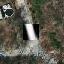
\includegraphics[width=0.15\columnwidth]{figs/labeloverlay.png}
\caption[Input patch and prediction]{Output prediction patch superimposed on input aerial image patch.}
\label{fig:system_data_patch}
\end{center}
\end{figure}

The system shares many similarities to the patch-based deep neural network presented by \cite{Mnih_aerial_images_noisy}. The system produces a patch of predictions given a patch of pixel values, where each value indicate the probability of the input pixel representing a road. Given a $64 \times 64$ aerial image patch the system computes a $16 \times 16$ patch of probabilities. The probabilities indicate the presence of road for the pixels found in the center of the aerial image patch. An example of input image patch and the output prediction patch can be seen in Figure \ref{fig:system_data_patch}.  \\

\begin{figure}[t]
\begin{center}
\includegraphics[width=1\columnwidth]{figs/system_overview.png}
\caption[Components of the system]{Components of the system.}
\label{fig:system_components}
\end{center}
\end{figure}

The actual implementation consists of two primary components, and an optional storage and graphical user interface web server component. The components and how they related, can be seen in Figure \ref{fig:system_components}. The storage and user interface component is not integral to the task of road detection, but has been a helpful aid when conducting experiments. Additionally, the patch dataset creator component is interchangeable, and can easily accommodate other varieties of segmentation datasets. In relation to the research questions, the patch dataset creator component is altered when investigating curriculum learning, and the loss function of the \ac{CNN} component is replaced when bootstrapping loss is applied. \\




\section{Semantic Segmentation with Convolutional Neural Network}
\label{sec:network}
This section will present the convolutional neural network in detail. \todo[inline]{Better and a slightly longer introduction to section}

\subsection{Patch-based approach}
This thesis formulates the problem of road segmentation in aerial images in the same manner  \cite{Mnih_roads_high_res_aerial_images} do \todo{Bad first paragraph. Wierd introduction}. This patch-based approach is presented in detail in Section \ref{sec:related_works}. In short, the convolutional neural network should learn the distribution \todo{Explained in related works. Tedious to repeat???}:

$$ p(m|s) = \prod_{i=0}^{w_m^2}p(m_i | s),  $$

where $p(m|s)$ denote a conditional probability of a label map patch given an aerial image patch. The patches $m$ and $p$ have been extracted from label image $M$ and aerial image $S$. Alternatively, the the label and image patch can be defined as $m =N(M_{i,j}, w_m)$ and $ s = N(S_{i,j}, w_s)$, where an area of $w_m \times w_m$ and $w_s \times w_s$ centered at location $(i, j)$ have been extracted from $M$ and $S$. By having a label patch $m$, the model can simultaneously make several predictions from the same context $s$, which is more effective than making a separate prediction per aerial image patch \todo{More effective to limit size of patches. Context is good but not too much. Assume conditional independence}. \\ 


The system is based on the deep neural network outlined by \cite{MnihThesis}. See Section \ref{sec:convolutional_networks_background} for background theory about \ac{CNN}. The network have three convolutional layers and two fully connected layers. This network architecture is depicted in Figure \ref{fig:conv}. The network predicts whether or not roads are present in a $16 \times 16$ pixel area in the center of  a $64 \times 64$ aerial image patch. The input patch is considerably larger than the output patch, so that the network can better utilize the context in the image. \\

The first layer performs convolution using $13 \times 13$ kernels. Only the first layer utilize max pooling, which reduces the number of inputs to the next layer as well as introducing some translational invariance in the model. The default kernel size in the second and third layer are $4 \times 4$ and $3 \times 3$, respectably. The output of the third convolutional layer is used as input to a fully connected neural network with a single hidden layer with 4096 units and an output layer. The latter contains 256 units where each output is the probability of a pixel representing a road.\\

\todo[inline]{stride}

The convolutional layers each have 64, 112 and 80 different feature maps, respectably. During training, these feature maps or kernels typically learn to respond to common local patterns in the input. The kernels in the first convolutional layer, for example, will learn to detect low level features in the aerial image, such as edges, colors and textures. This happens because the \ac{CNN} employ parameter sharing by convolving the same kernel across the input data, forcing the model to find local image features. The 64 feature maps from the first layer of a trained model, can be viewed in Figure \ref{fig:convoluional_first_layer_visualization}. Many of the kernels seem to have developed into something similar to Gabor filters, which are effective at detecting edges at certain orientations. Coincidentally, oriented two-dimensional Gabor functions are widely used to model the response from simple-cell receptive fields in the primary visual cortex. \\

%Read this before citing
%\citep{Ringach_gabor_spatial}
%http://jn.physiology.org/content/jn/88/1/455.full.pdf

\begin{figure}
\begin{center}
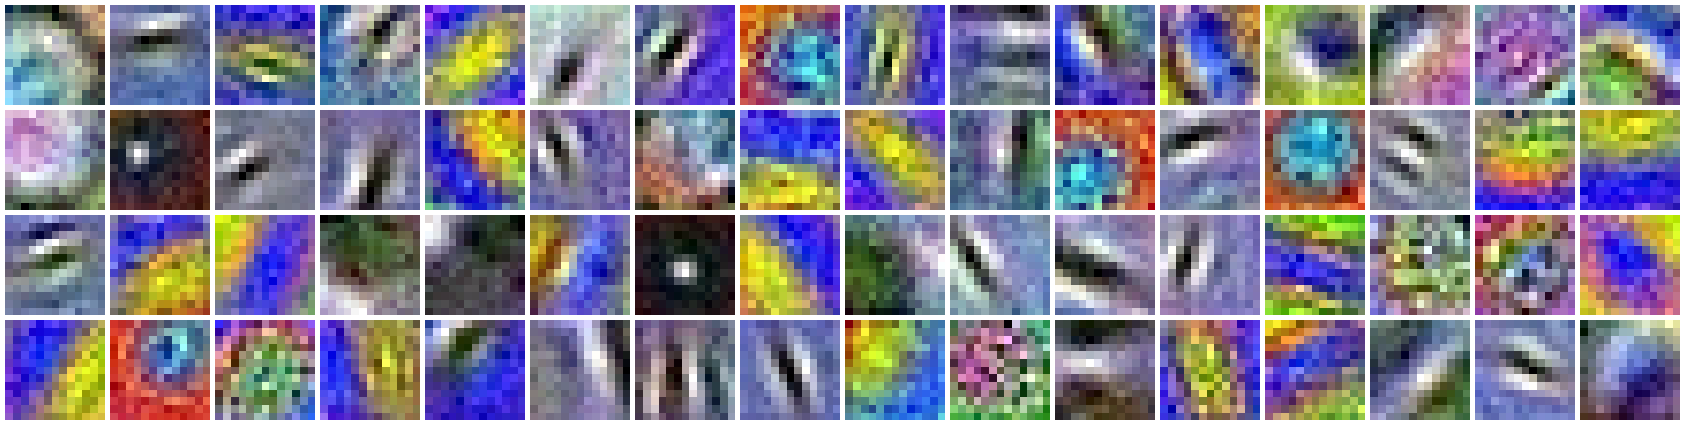
\includegraphics[width=1\columnwidth]{figs/network/Filter_unblurred.png}
\caption[Visualization of filter map]{Visualization of filter maps from the first convolutional layer of a trained network.}
\label{fig:convoluional_first_layer_visualization}
\end{center}
\end{figure}

Common for both convolutional layers and fully connected layers, are the use of a non-linear activation function, which allow the network to learn non-linear decision boundaries \todo{Fact check}. To compute the outgoing activation of any unit in the network, the incoming weights are first summed with the activations coming from either the input or the previous layer. Then, a bias is added, before feeding the result through the activation function. This is typically denoted \todo{Totally bad word}:

$$ y = \sigma(aw + b),$$

\noindent where $a$ and  $w$ is the unit's incoming activations and weights, $b$ is the bias and $\sigma$ is the non-linear activation function.\\

In the default hyperparameter configuration of this system, the output layer apply the logistic activation function, while the \ac{ReLU} activation function is used by the input and hidden layers. The logistic activation function is appropriate for the output layer, because it squashes any input to be between the value of 0 and 1. This is useful for the road detection system, where the activation of each output unit should predict a probability of whether the corresponding aerial image patch pixel belong to the road class or not. The \ac{ReLU}, however, has been used for all other layers. This activation function has been shown to be especially effective for deep neural networks \todo{Bad sentence and paper}.  The activation functions are displayed in Figure \ref{fig:activation_functions}.\\

\begin{figure}[h]
\begin{subfigure}{0.45\textwidth}
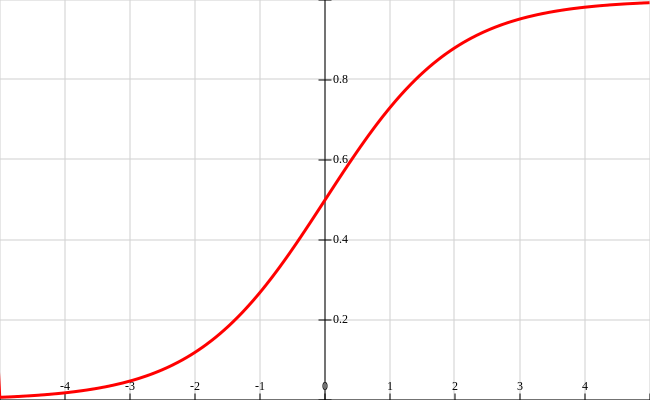
\includegraphics[width=\linewidth]{figs/sigmoid2.png}
$$ y = \frac{1}{1+ e^{-x}}$$
\caption{Logistic} \label{fig:activation_sigmoid}
\end{subfigure}
\hspace*{\fill} % separation between the subfigures
\begin{subfigure}{0.45\textwidth}
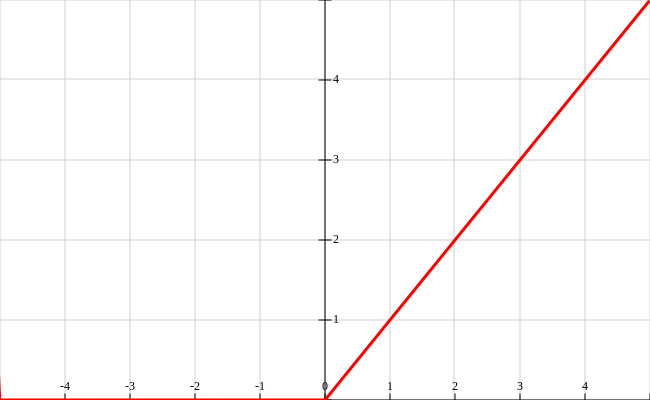
\includegraphics[width=\linewidth]{figs/relu2.png}
$$ y = \text{max}(0, x) \frac{}{}$$
\caption{Rectified linear unit} \label{fig:activation_relu}
\end{subfigure}
\hspace*{\fill} % separation between the subfigures
\caption{Activation functions} \label{fig:activation_functions}
\end{figure}


The specific network configuration described in this section, is the default configuration used in experiments found in Chapter \ref{cha:ResearchAndResults}. However, the network architecture can easily be changed through a configuration file. All configurable parameters and default values are listed in Table \ref{tab:network_parameters}.\\

\begin{table}[htp]
\caption{Hyperparameters for \ac{CNN}}
\begin{center}
\begin{adjustbox}{max width=\textwidth}
\begin{tabular}{+l ^l ^l}\hline
\rowstyle{\bfseries}
  Parameter & Description & Value\\\hline
  $K^{(l)}$ & Number of kernels for convolutional layer $l$ & 64, 112, 80 \\
  $CLF^{(l)}$ & Filter size of convolutional layer $l$ & (13,13),(4,4),(3,3) \\
  $CLS^{(l)}$ & Stride amount of convolutional layer $l$ & (4,4),(1,1),(1,1) \\
  $CLP^{(l)}$ & Pool size of convolutional layer $l$ & (2,2),(1,1),(1,1) \\
  Cost function & Function that is minimzed each iteration & Cross entropy \\
  Epochs & How many epochs \ac{CNN} will train for. & 100 \\
  $\sigma^{(l)}$ & Transfer function for each layer $l$ & Leaky ReLU x4, sigmoid x1 \\
  $h$ & Number of neurons in hidden layer. & 4096 \\
  $p^{(l)}$ & Dropout rate for a layer $l$ & 1.0, 0.9, 0.8, 0.5, 1.0 \\
  $a$ & Learning rate & 0.0014 \\
  $a_{decrease}$ & learning rate decrease factor & 0.95 \\
  $\lambda$ & L2 Weight decay strength & 0.0001 \\
  $m$ & Momentum & 0.9 \\
  $b$ & Batch size & 64 \\\hline
\end{tabular}
\end{adjustbox}
\end{center}
\label{tab:network_parameters}
\end{table}


\subsection{Optimization}
%\url{http://cs231n.github.io/neural-networks-3/}
%http://www.cs.toronto.edu/~tijmen/csc321/slides/lecture_slides_lec6.pdf}
%http://arxiv.org/pdf/1212.0901v2.pdf
%http://stats.stackexchange.com/questions/179915/whats-the-difference-between-momentum-based-gradient-descent-and-nesterovs-ac
The model parameters are optimized with a special form of \ac{SGD}, called Nesterov momentum stochastic gradient decent, and has an improved stability and faster convergence compared to standard \ac{SGD} \citep{Bengio_advances_optimizing}. The standard momentum approach extend the gradient update step, by introducing velocity. The loss can be interpreted as a hilly error surface where loss optimization can be viewed as a particle gaining and losing velocity while interacting with the landscape. When the loss optimization has gained velocity, it will stop doing purely steepest decent, and results in a smoother decent with less oscillations. Basically, instead of directly using the gradient to move in the landscape, the gradient will influence the velocity. The only hyperparameter associated with momentum is $m$, which damps the velocity, and can be interpreted as friction inflicted on the particle \todo{INflicted on the particle?}. \\


Nesterov momentum is a variation of momentum. Unlike standard momentum, the Nesterov method first makes a step in the direction of the accumulated velocity, and then makes a correction of the velocity based on the new location. In standard momentum a correction to the velocity is made before taking a step. The Nesterov gradient is defined by the following update rule:

\begin{flalign*}
     &v_{t} = mv_{t-1} - a \nabla f(\theta_{t-1} + m v_{t-1}) \\
     &\theta_t = \theta_{t-1} + v_t,
\end{flalign*}

\noindent where $\theta_t$ is the model parameters, $v_t$ the velocity, $m$ the momentum decay, $a$ the current learning rate and $\nabla f(\theta)$ is the gradient.\\

Furthermore, the system also support RMSProp which keeps a running average of the gradient magnitude for every weight. This is used to adaptively adjust the learning rate of each weight. Compared to regular \ac{SGD}, this will result in a faster convergence. \todo{Paper detailing RMSprop}\\ 

All the above mentioned optimization approaches have an important hyperparameter in common, and that is the learning rate $a$. In this implementation the learning rate is annealed over time, by step decay. The learning rate is decreased in regular intervals of epochs by some factor $a_{decrease}$ during optimization. \\

\todo[inline]{Learning and negative log likelihood?. Optimization of the loss. So the loss is negative log likelihood}
%http://neuralnetworksanddeeplearning.com/chap3.html crossentropy!!

\subsection{Regularization}
To avoid overfitting the training data, and hopefully achieve better generalization, different regularization schemes are applied during optimization, such as L2 weight decay, early stopping, and dropout. The model's task is to learn the regularities found in the mappings between the data and labels in the training set. However, the training set also contain sampling errors and accidental patterns not relevant to the task at hand. Without regularization, a model will learns the useful, but also the erroneous regularities a bit too well, and can therefore start to overfit the data. \\

L2 regularization is a weight decay method which applies a loss function penalty to prevent weights in the network from growing large. This is achieved by adding an extra term, $\lambda\sum_{i=0}^{|w|} w_i^2$ to the loss function, which penalize large valued weights, and encourages a smoother parameter configuration \citep{Hinton_regularization}. The strength of the weight decay is controlled by the $\lambda$ hyperparameter, which is typically is set to a low value \todo{Ok to cite lecture note???}.\\

Early stopping stops the optimization process when performance on the validation set starts to consistently decrease. When the validation loss stagnates or starts to increase in value, the method waits for a certain number of iterations before stopping the training process. There are three parameters that controls the early stopping behaviour, \textit{initial patience}, \textit{improvement threshold} and \textit{patience increase}. The first parameter controls how many iterations the training should run for, regardless of validation loss improvements. The second parameter dictates the required amount of improvement of the current validation loss compared to the best previously seen validation loss, before incrementing the patience variable. The latter parameter decide the increment factor of the patience. The patience, or how many additional iterations early stopping will wait for a validation loss improvement, is defined as $\textit{patience} = max(\textit{patience}, \textit{iteration} \times \textit{patience increase} )$ \todo{Paper, and is formula really necessary???}\\
%http://link.springer.com/chapter/10.1007/3-540-49430-8_3

The dropout method forces the units to rely less on each other, by randomly disabling units in the network during training. This encourage units to encode independently useful information, since dropout penalize co-adaptation between units \citep{Srivastava_dropout}. Dropout can also be viewed as an ensemble method approximation. By randomly removing subsets of units from the network, an exponential number of parameter sharing subnetworks are trained simultaneously. This is less computationally expensive than training an ensemble of many individual neural networks. At test time, the predictions of these subnetworks are combined by an approximate averaging method \todo{Bad way to say this}. This is done by having the neural network produce predictions without dropping any units. Because all units make contributions, the weights of the network have to be scaled down. If a unit is retained with a probability of $p$ during training, the outgoing weights of that unit should be multiplied by $p$ at test time. Each layer $l$ has an unique dropout rate parameter, $p^{(l)}$, which controls the probability of dropping an unit at that layer.  In the \ac{CNN} implementation, dropout has been implemented with some minor tweaks: \\

\todo{VERY BAD}
\begin{flalign*}
     &Y = \frac{1}{p^{(l)}} R \sigma(W^{(l)}X + B^{(l)}),
\end{flalign*}

\noindent where $W$ and $B$ are the weights and biases in layer $l$, $X$ denote the input potentials and f(z) is the activation function. $R$ is a vector of independent Bernoulli random variables each having a probability of $p^{(l)}$ being 1. Instead of multiplying the outgoing weights at test time, the output potentials during training are divided by $p^{(l)}$, which should essentially give the same scaling effect.\\


\subsection{Data preprocessing}
The datasets used in this thesis contains aerial images and road label maps that are very large. Each image is typically around $1500 \times 1500$ pixels in size, which is arguably to large for the model to use directly as input. Smaller patches of examples are therefore extracted from these larger images. From each image a certain number of data patches and label patches of $64 \times 64$ and $16 \times 16$ are extracted randomly and added to a patch dataset.\\

However, before extracting patches, each aerial image and road label map is rotated by a random number of degrees between 0 and 360 degrees. This is necessary because of orientation bias in the datasets \todo{DO they?}. In many cities the road network is often constructed in a grid pattern, which leads to roads having certain orientations. Without random rotations of the training data, the model might become better at detecting roads only at certain orientations \citep{Mnih_roads_high_res_aerial_images}. Each image is therefore rotated by a random angle before extracting patches, which results in a patch training set that encourages the model to learn invariance to orientation \todo{A bit icky. Invariance to orientation shoulds wrong.}.\\

Another data augmentation method utilized when constructing the patch training set is flipping. This is a common method for artificially increase the size of the dataset \citep{Krizhevsky_imagenet}. Since the dataset contains aerial imagery that depict landscape from a top-down perspective, the patches can both be flipped vertically and horizontally \todo{Something missing here}.\\

Contrast normalization is also applied to every patch. Each patch is normalized by subtracting the mean pixel value from the pixels of a patch, and then dividing the result by the standard deviation found for all pixels in the dataset.\\

Additionally, the datasets exhibit some class imbalance \citep{Japkowicz_class_imbalance}, which can be problematic since the model might decide to prioritize loss minimization of the high-occurence classes and ignore low-occurring classes. Random sampling of the datasets, lead to a large imbalance between road examples and non-road examples. The proportion of patches containing road according to the labelling, range between 8\% and 25\%\todo{Check numbers}, depending on the dataset. This is solved by artificially increasing the proportion of road examples, when sampling the patch dataset. This method is not applied to the test and validation patch set, and will therefore retain their natural class distribution\todo{Improve language}.\\

\section{Curriculum learning}
\label{sec:curriculum_learning}
The curriculum learning method presented by \cite{Bengio_curriculumlearning}, showed that presenting the dataset in a certain order yielded better generalization as well as faster convergence. Similar to a school curriculum, easier concepts are taught before harder concepts, which most likely is the preferred way of learning for humans \citep{Khan_human_teach}. This translates to having the learning algorithm do optimization on a dataset consisting of "easier" examples, before introducing "harder" examples. Continuing this analogy, there is a teacher who decides the curriculum by judging how easy concepts is to grasp. For some datasets, such as language modelling datasets, the role of the teacher can easily be performed by a human. In language modelling tasks, a viable curriculum strategy is to start training using a simple dataset containing examples with only a limited vocabulary, and then gradually grow the allowed vocabulary. However, similar curriculum strategies are harder to identify for datasets involving images. The solution is therefore to outsource the job of curriculum teacher, to a supervised learning algorithm.  \\

In this thesis, aerial image datasets are used. Based purely on color image patches, a supervised learning algorithm should be able to detect and segment roads found in these patches. A curriculum strategy involving this type of data is harder to identify. Is curved roads segment harder to learn for a machine learning algorithm than a straight road segment? Or are roads in rural scenes easier to learn than roads in an urban setting? What configurations of pixel intensities are easier? It is hard for a human to identify features in images which a machine learning algorithm would consider easier to learn. \\


Hence, a classifier is first trained on the available examples and given the role of the teacher. The classifier, regardless of competence, will generate predictions which is used in a difficulty estimation of each example. The difficulty estimation is simply based on the amount of disagreement between the teacher's prediction and the label of the example. The difficulty estimator is defined below:  \\

 \begin{flalign*}
  &  d(y, q) = \frac{1}{w_m^2}\sum_{i=0}^{w_m^2} |y_i - \mathbb{1}_{q_i > r} |,  \\
 \end{flalign*}
 
 
\noindent where $q$ is the curriculum teacher's prediction, $y$ is the label. The $\mathbb{1}_{q_i > s}$ is a threshold operator, where $r$ is the threshold value which gives the best precision and recall breakeven for the curriculum teacher classifier. The operator essentially, creates a binary image patch from the prediction probabilities. The estimator compute the average value from the $w_m \times w_m$ patch of label pixels and prediction probabilities. Even though the estimator has been customized to the patch-based approach of aerial road detection, the method can easily be adopted to other types of datasets. This curriculum strategy can therefore be considered generally applicable. The disagreement between a prediction created by a trained classifier and a label, can probably be computed for most datasets. \\

An interesting thing to note, is that a very competent teacher classifier, computing a high difficulty score for an example, might indicate that the example's label is inconsistent.   \\

The implementation of curriculum learning, involve $S$ training set stages. Each stage $\theta$ only contains examples where $d(y, q) < D_{\theta}$, in which the difficulty threshold $ D_{\theta} > D_{\theta -1}$ for all stages $ \theta > \theta -1$. Each subsequent stage, therefore contain examples with a broader range of difficulties \todo{Weird}. In the final stage $S$, the threshold $D_{S}$ is typically set to 1, which result in every example being added to the patch dataset. This stage has a training distribution equal to what a patch dataset created from random sampling would have had.\\

The supervised learning algorithm, is gradually exposed to harder examples by stage switching. The classifer is first optimized with the examples in the first stage, which has the lowest difficulty threshold. At epoch $t_{start}$, the next stage replaces the existing training set by random sampling without replacement. Following stages are mixed into the training set every $t_{stage}$ epoch, until the model has trained with examples from all stages. The hyperparameters and default values for curriculum learning are listed in  Table \ref{tab:curriculum_parameters}. \\

\begin{table}[htp]
\caption{Hyperparameters for curriculum learning.}
\begin{center}
\begin{adjustbox}{max width=\textwidth}
\begin{tabular}{+l ^l ^l}\hline
\rowstyle{\bfseries}
 		 Parameter & Description & Value\\\hline
 		 $S$ & Number of stages & 2 \\
 		 $D_\theta$ & Threshold value for difficulty estimate for stage $\theta$ & 0.25, 1.0 \\
 		 $t_{start}$ & What epoch to load stage 1 & 50 \\
 		 $t_{stage}$ & Load subsequent stage after every $t_{stage}$ epoch & 50 \\\hline
\end{tabular}
\end{adjustbox}
\end{center}
\label{tab:curriculum_parameters}
\end{table}

\section{Bootstrapping loss}
\label{sec:bootstrapping_loss}
Normally, the loss function calculates the loss assuming the labels are correct. But many datasets contain label noise, which will result in the learner being penalized for making a correct prediction if the label happens to be inconsistent. According to \cite{Reed_noisy_labels_bootstrapping}, tweaking the loss function by incorporating the network's own predictions can yield improved robustness to inconsistent labelling. Whereas other approaches \citep{Mnih_aerial_images_noisy}\citep{Sukhbaatar_noisy_network_learning} explicitly model the noise distribution, the proposed loss function utilizes the implicit knowledge acquired by the network during optimization. The bootstrapping method, computes the loss by a convex combination of the model prediction q and the label y. Additionally, this thesis propose a variation of the bootstrapping loss function, which only incorporate confident predictions. \\

The bootstrapping loss function, use the current model prediction $q$ and the noisy training label $y$ in a convex combination, which result in a modified target. Except for this, the loss function is similar to cross entropy\todo{Is it though?}. The model prediction's contribution to the convex combination is decided by the $\beta$ parameter. The bootstrapping loss for the aerial road detection system is defined below:

 \begin{flalign*}
  \mathcal{L}_{hard}(q,y) =&  - \sum\limits_{i=1}^{w_m^2} [\beta y_i + (1-\beta)\mathbb{1}_{q_i > 0.5}]log(q_i)  \\
                    & - \sum\limits_{i=1}^{w_m^2} [\beta (1-y_i) + (1-\beta)(1-\mathbb{1}_{q_i > 0.5})]log(1 - q_i) 
 \end{flalign*}

\noindent where $\mathbb{1}_{q_i > 0.5}$ is the MAP estimate of the model prediction $q$ \todo{Why is this important?}. For the task of road detection it is simply a threshold operation. All probabilities above 0.5 are set to 1, otherwise 0. This is the reason why this loss function is denoted hard. A soft version of bootstrapping where the predictions $q_i$ are used directly, has also tested by \cite{Reed_noisy_labels_bootstrapping} , but generally performed worse than the bootstrapping hard variant.\\

Bootstrapping loss combined with gradient descent, results in an EM-like algorithm. In the E-step the modified targets are generated, whereas in the M-step the network weights are adjusted to better predict the modified targets. The goal is for the learner to rely less on the inconsistent labels, and develop more consistent implicit knowledge, which in turn further improves the quality of the modified targets.\\
 
Since, the task involves the binary task of discriminating road pixels from non-road pixels, a slightly modified version of bootstrapping is also tested in the thesis. This approach is named confident bootstrapping, since all model predictions between 0.2 and 0.8 are ignored. Only predictions that the learner have a high confidence in, are allowed to contribute in the convex combination. An added benefit of this loss function, is the possibility of increasing the factor $\beta$. The confident bootstrapping loss function is denoted:

  \begin{flalign*}
  \mathcal{L}_{confident}(q,y) =&  - \sum\limits_{i=1}^{w_m^2} [\beta y_i + (1-\beta)\mathbb{1}_{q_i > 0.8}]log(q_i)  \\
                    & - \sum\limits_{i=1}^{w_m^2} [\beta (1-y_i) + (1-\beta)(\mathbb{1}_{q_i < 0.2})]log(1 - q_i) 
 \end{flalign*}
 
\noindent where $\mathbb{1}_{q_i > 0.8}$ and $\mathbb{1}_{q_i < 0.2}$ are threshold operations which only keep fairly confident predictions. For the task of road detection, this translates to saying pixel predictions above 0.8 are most likely road pixels, and predictions below 0.2 are very likely to be not be a road pixel.\\

In the implementation, the $\beta$ parameter is annealed often from 1.0, down to the minimum value of $\beta_{min}$, after $\beta_{start}$ epochs. This is because the learner should have some implicit knowledge before using it's predictions to modify the target. Similar to \cite{Sukhbaatar_noisy_network_learning}. This is probability not important for confident bootstrapping \todo{OMG, so bad}. The configurable parameters for bootstrapping can be found in Table \ref{tab:bootstrapping_parameters}

\begin{table}[htp]
\caption{Hyperparameters for bootstrapping loss}
\begin{center}
\begin{adjustbox}{max width=\textwidth}
\begin{tabular}{+l ^l ^p{3.5cm}}\hline
\rowstyle{\bfseries}
 		 Parameter & Description & Value\\\hline
 		 Cost function & Modified cost function  & bootstrapping or confident boostrapping \\
 		 $\beta$ & Mix factor  & 1.0 \\
 		 $\beta_{min}$ & Minimum mix factor & 0.90 \\
 		 $\beta_{start}$ & When to start mixing & 60 \\\hline
\end{tabular}
\end{adjustbox}
\end{center}
\label{tab:bootstrapping_parameters}
\end{table}

\section{Datasets}
\label{sec:datasets}
  When testing the bootstrapping loss function and curriculum learning, as well as measuring the performance of the road detection system, two datasets have been utilized. Both datasets involve the task of semantic segmentation of images, more precisely, the task of extracting roads from aerial images. The first dataset, Massachusetts Roads Dataset, provided by \cite{MnihThesis}, has been used in several works. The second dataset, Norwegian Roads Dataset, was specifically made for this thesis, and was generated from publicly available data. Differences, similarities, and challenges of employing these datasets will be further discussed below.\\

\subsection{Massachusetts Roads Dataset}
The Massachusetts Roads Dataset contains aerial images depicting urban, suburban, and rural areas in the state of Massachusetts, USA. In all, the dataset consists of 1171 aerial images, where each image is $1500\times 1500$ pixels in size. 1108 of these images have been randomly assigned to the training set. The remaining 49 and 14 images can be found in the test and validation set. The dataset covers an area of approximately 2600 square kilometers in total, which gives a \ac{GSD} of 1.0 meter per pixel.\\

Each aerial image has an accompanying identically sized binary label image, which indicates whether a pixel in the aerial image belongs to either the road or non-road class. Road centerline vectors retrieved from the OpenStreetMap project were used to generate the label images. The vectors were rasterized as white lines with a line thickness of 7 pixels \citep{MnihThesis}, which, based on the \ac{GSD}, is equivalent to 7 meters on the ground. An aerial image and label image pair from this dataset can be seen in Figure \ref{fig:mass_roads_example}.\\

\begin{figure}
\begin{subfigure}{0.48\textwidth}
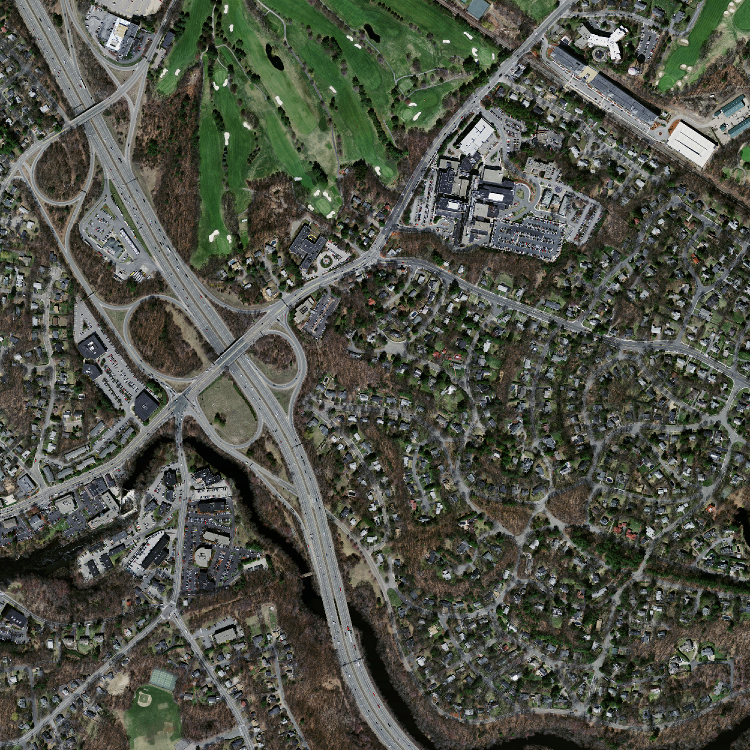
\includegraphics[width=\linewidth]{figs/datasets/Mass_roads_data_example2.png}
\caption{Aerial image} \label{fig:mass_roads_example_data}
\end{subfigure}
\hspace*{\fill} % separation between the subfigures
\begin{subfigure}{0.48\textwidth}
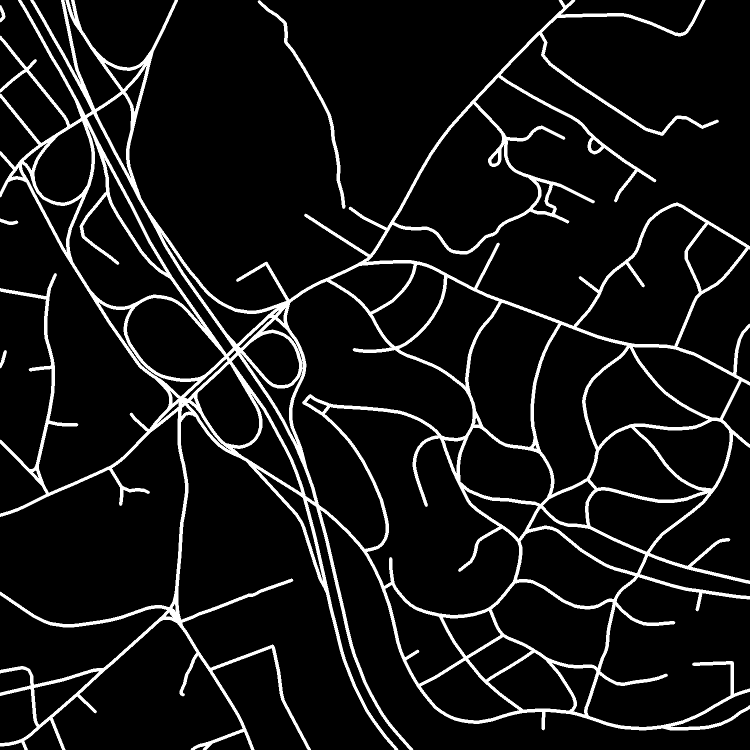
\includegraphics[width=\linewidth]{figs/datasets/Mass_roads_label_example2.png}
\caption{Label image} \label{fig:mass_roads_example_label}
\end{subfigure}
\hspace*{\fill} % separation between the subfigures
\caption[Massachusetts Roads Dataset]{Image and label example taken from test set in Massachusetts Roads Dataset.} \label{fig:mass_roads_example}
\end{figure}


There are many reasons for using this dataset to conduct experiments related to the research questions.  The task involves semantic segmentation of roads based exclusively on aerial color images. This is arguably a hard task, and might justify the use of a large model for training, such as a \ac{CNN}. The dataset has also been used in other works, which enables comparison of the results obtained in this thesis to the results obtained in other works. Additionally, the labels have been generated from existing map data, and therefore contain many instances of naturally occurring inconsistent labeling. This is compelling in relation to the research questions of this thesis.\\

Aerial image datasets typically suffer from two distinct types of label noise, which \cite{Mnih_aerial_images_noisy} have named omission and registration noise. The dataset is generated from existing map data, which has \todo{have?} some deficiencies when coupled with supervised learning. There are many instances of omission noise in this dataset, where smaller roads and parking areas have not been marked as road class pixels in the label images. These omissions are most likely perfectly acceptable for map purposes, but might negatively impact the performance of a classifier.  For instance, unlabeled paved areas that share a high spectral similarity to roads could be considered inconsistently labeled. These label errors might compel the classifier to minimize the loss by learning complicated distinctions between surfaces that are essentially the same thing.\\

There are also instances of registration noise in this dataset. This happens when there are misalignments between the roads found in the aerial images and the road centerline vectors from the map data. Additionally, the road centerline vectors have, in many cases, been rasterized with the incorrect line thickness, which might cover too much or not enough depending on the road's lane width. The result is a lot of aerial image pixels that have been assigned the wrong class, which might impact the learning procedure negatively. Just like omission noise, slightly misaligned road centerline vectors does \todo{do? If so sounds probably placed weirdly} probably not matter too much for map purposes, whereas they create a lot of inconsistent examples in a machine learning dataset.


%\subsection{Massachusetts Roads Dataset}

\subsection{Norwegian Roads Dataset}
In addition to the Massachusetts Roads Dataset \citep{MnihThesis}, the proposed methods have been tested with the Norwegian Roads Dataset. This dataset was constructed from aerial images retrieved from Kartverket, which depicts both rural, suburban, and urban areas from different locations in Norway. The entire dataset consists of 1225 aerial images, each being $1536\times 1536$ pixels in size. 1100 of them have been randomly assigned to the training set, 75 to the test set, and the remaining images were put in the validation set. Even though there are more aerial images in this dataset compared to the Massachusetts Roads Dataset, it only covers an area of around 1910 square kilometers. This is due to a much lower \ac{GSD} of about 0.66 meters per pixel. \\


The label images in this dataset have been generated from road centerline vectors found in the publicly available topographic vector database, N50, provided by \cite{Kartverket}. Unlike the Massachusetts Roads Dataset, the centerline vectors have been rasterized with a variable line thickness. This is possible because all road segments in N50 have a set of properties, which can be utilized to determine a custom line thickness. The actual thickness of each road type has been based on numbers found in a road specification manual published by the Norwegian Public Roads Administration \citep{Norwegian_road_manual}. The road segment properties and line thickness for each road type are listed in Table \ref{tab:road_rules}. Roads that are underground and cannot be seen from aerial imagery have also been removed from the rasterized label images.\\

The aerial images have been taken from over 30 different locations in Norway, and offers a large variety of topographical features. There are images depicting coastlines, rivers, mountain terrains, snow, cultivated land, and forests. Compared to Massachusetts Roads Dataset, the aerial images of this dataset have been sampled from a much larger area. Furthermore, the aerial images might present a challenge in terms of image quality. Some of the images vary \todo{varies?} in terms of color balance and image contrast. There are also aerial images that have been stitched together from images captured by aerial surveys conducted at different occasions.\\

The quality of the generated label maps might also present a challenge to a machine learning algorithm. There are both omission and registration errors present in many of the label images. Compared to the Massachusetts Roads Dataset there is a much higher degree of registration noise. The road centerlines in N50 generally appear more coarse, and result in less overlap between roads in the aerial image and the raster lines in the label image. This is especially evident in road centerline vectors for divided highways. Instead of having centerline vectors for both roadways, there is only one placed between the roadways on the median. Visual examples of missing and misplaced labels can be seen in Figure \ref{fig:norwegian_roads_examples_n50}.\\

\begin{figure}[h]
\begin{subfigure}{0.31\textwidth}
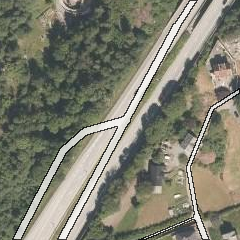
\includegraphics[width=\linewidth]{figs/datasets/nor_examples/1191_highway_n50.png}
\caption{Divided highways} \label{fig:norwegian_roads_highway_n50}
\end{subfigure}
\hspace*{\fill} % separation between the subfigures
\begin{subfigure}{0.31\textwidth}
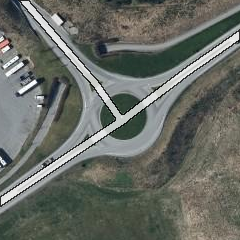
\includegraphics[width=\linewidth]{figs/datasets/nor_examples/1177_roundabout_n50.png}
\caption{Roundabout} \label{fig:norwegian_roads_roundabout_n50}
\end{subfigure}
\hspace*{\fill} % separation between the subfigures
\begin{subfigure}{0.31\textwidth}
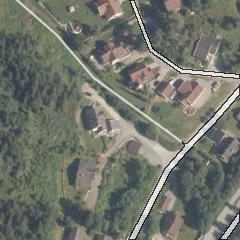
\includegraphics[width=\linewidth]{figs/datasets/nor_examples/1157_missing_n50.png}
\caption{Private road} \label{fig:norwegian_roads_missing_n50}
\end{subfigure}
\hspace*{\fill} % separation between the subfigures
\caption[Inconsistent labelling in Norwegian Roads Dataset N50]{Examples of inconsistent labelling found in the Norwegian Roads Dataset N50.} \label{fig:norwegian_roads_examples_n50}
\end{figure}

In addition to the set of label images generated from N50, the dataset also includes an alternate set of label images generated from the road centerline vector database, Vbase \citep{Kartverket_vbase}. This database has more accurate road centerline vectors. There are still omission and registration errors present in this label image set, but to a less extent. Surfaces that share spectral similarities to asphalt, such as private roads and parking areas, have not been marked, similar to the Massachusetts Roads Dataset. The difference in accuracy between N50 and Vbase can be seen by comparing Figure \ref{fig:norwegian_roads_examples_n50} and Figure \ref{fig:norwegian_roads_examples_vbase}. A minor downside of using this alternate vector database is that Vbase provides fewer road segment properties, which have resulted in a smaller set of line thicknesses applied to the label images.\\

\begin{figure}[h]
\begin{subfigure}{0.31\textwidth}
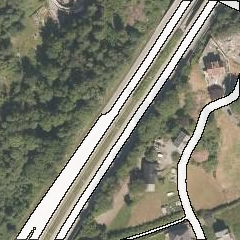
\includegraphics[width=\linewidth]{figs/datasets/nor_examples/1191_highway_vbase.png}
\caption{Divided highways} \label{fig:norwegian_roads_highway_vbase}
\end{subfigure}
\hspace*{\fill} % separation between the subfigures
\begin{subfigure}{0.31\textwidth}
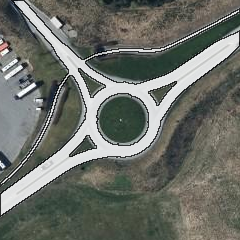
\includegraphics[width=\linewidth]{figs/datasets/nor_examples/1177_roundabout_vbase.png}
\caption{Roundabout} \label{fig:norwegian_roads_roundabout_vbase}
\end{subfigure}
\hspace*{\fill} % separation between the subfigures
\begin{subfigure}{0.31\textwidth}
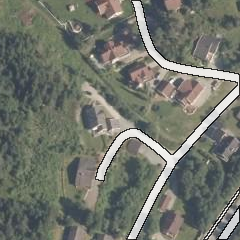
\includegraphics[width=\linewidth]{figs/datasets/nor_examples/1157_missing_vbase.png}
\caption{Private road} \label{fig:norwegian_roads_missing_vbase}
\end{subfigure}
\hspace*{\fill} % separation between the subfigures
\caption[Road centerline vector quality of Vbase]{Examples of road centerline vector quality in Vbase.} \label{fig:norwegian_roads_examples_vbase}
\end{figure}

\begin{table}[htp]
\caption[Raster line thicknesses for the Norwegian Roads Dataset]{Raster line thickness and road segment filtering rule for each type of road. A margin of 10\% is removed from the line thicknesses, which are based on numbers found in the road specification manual.}
\begin{center}
\begin{adjustbox}{max width=\textwidth}
\begin{tabular}{+l ^l ^r}\hline
		 \rowstyle{\bfseries}
 		 Road type & Road segment property & Line thickness\\\hline
 		 Dirt road & OBJTYPE=Traktorveg & 2.50 m\\
 		 Trail & OBJTYPE=Sti & 1.50 m\\
 		 pedestrian road & OBJTYPE=GangSykkelveg & 2.25 m\\
 		 Highway & MOTORVEGTYPE=motorveg & 10.80 m\\
 		 International E-road network & VEGKATEGORI=E & 6.30 m\\
 		 Norwegian national road & VEGKATEGORI=R & 5.85 m\\
 		 municipal road & VEGKATEGORI=K & 4.95 m\\
 		 Private road & VEGKATEGORI=P & 3.50 m\\\hline
\end{tabular}
\end{adjustbox}
\end{center}
\label{tab:road_rules}
\end{table}

The dataset was constructed by using QGIS, an open source geographic information system application. The application enables viewing and editing of map data, but also provides a Python interface. A script to create label images was developed, taking the map coordinates associated with each corner of an aerial image, and generating a raster image of road centerline vectors found inside that area. The resulting raster images can be used as target maps in supervised learning. \\

\begin{figure}
\begin{subfigure}{0.32\textwidth}
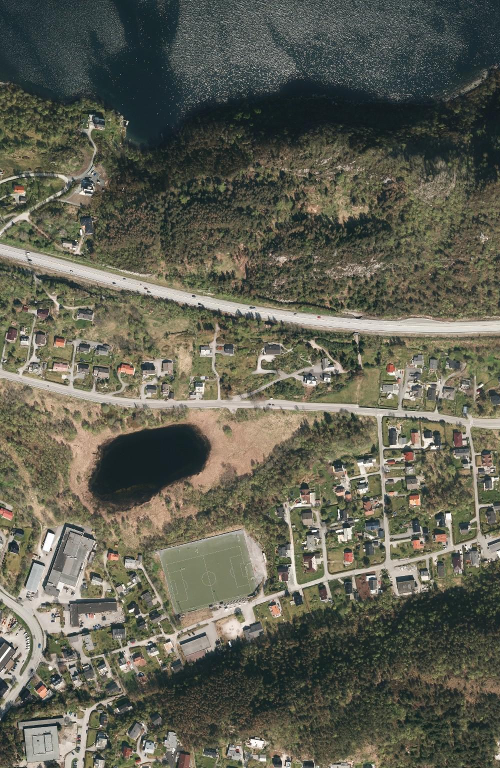
\includegraphics[width=\linewidth]{figs/datasets/Norwegian_roads_data_example2.png}
\caption{Aerial image} \label{fig:norwegian_roads_example_data}
\end{subfigure}
\hspace*{\fill} % separation between the subfigures
\begin{subfigure}{0.32\textwidth}
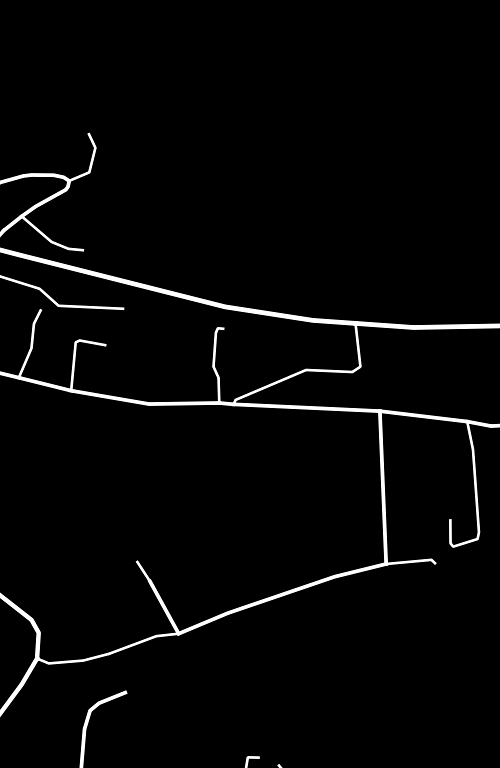
\includegraphics[width=\linewidth]{figs/datasets/Norwegian_roads_label_example2.png}
\caption{Label image} \label{fig:norwegian_roads_example_label}
\end{subfigure}
\hspace*{\fill} % separation between the subfigures
\begin{subfigure}{0.32\textwidth}
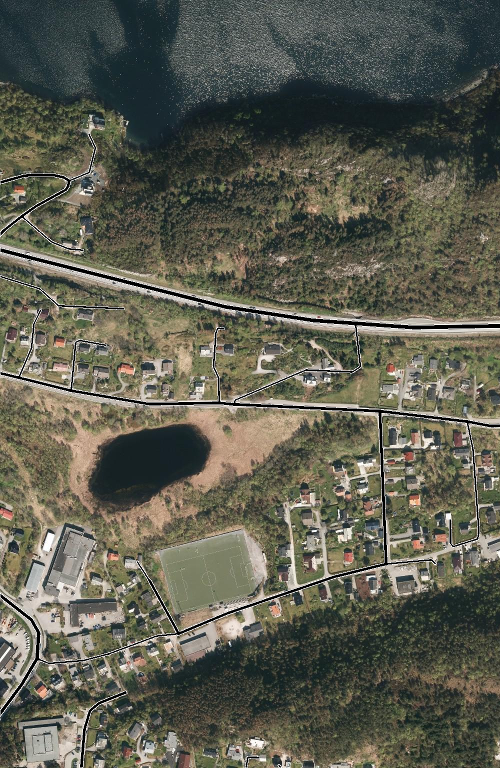
\includegraphics[width=\linewidth]{figs/datasets/Norwegian_roads_overlay_example2.png}
\caption{Overlay image} \label{fig:norwegian_roads_example_overlay}
\end{subfigure}
\hspace*{\fill} % separation between the subfigures
\caption[Example from Norwegian Roads Dataset N50]{Example from test set in Norwegian Roads Dataset N50.} \label{fig:norwegian_roads_example}
\end{figure}

An aerial image and its corresponding label image from the Norwegian Roads Dataset N50 can be seen in Figure \ref{fig:norwegian_roads_example}. Figure \ref{fig:norwegian_roads_example_overlay} shows the same label image superimposed on the aerial image. Observe that some roads are missing from the label image, as well as the ground truth not covering the roads properly. \\


\section{Implementation Details}
\label{sec:methods_implementation_details}
The road detection system was written with the Python programming language, and uses the open source library Theano \citep{bergstra_theano}. Theano enables the developer to define and evaluate mathematical expressions involving tensors. The library implements several useful features for developing \ac{CNN}s, such as backpropagation, convolution, and max pooling. Training deep neural networks on a \ac{GPU} can be considerably faster than on a \ac{CPU}, and Theano can utilize both the \ac{CPU} and \ac{GPU} without making any modifications to the code.\\

However, the use of a \ac{GPU} was key in making the experiments feasible to run. The system has a a lot of adjustable parameters and requires a big dataset in order to generalize well to the task of road detection. The experiments were conducted on a machine with a Nvidia GTX 980 \ac{GPU} with 4 gigabytes of video memory. \\

Because the size of the training set in many cases exceeded the capacity of the video memory, the video memory only contains the model, validation set, test set, and a subset of the training set at any given time during training. A switching mechanism was implemented, where chunks from the training set residing in main memory are loaded onto the \ac{GPU} sequentially during an epoch of training.\\

The system also has a large number of hyperparameters which can be changed by the user. This includes learning rate, network architecture, backpropagation method, dropout rates, curriculum and bootstrapping specific parameters, and more. These values can be accessed and modified in the system's config.py file. \\

The code for the road detection system as well as the machine learning monitoring interface are publicly available at 
\url{https://github.com/olavvatne/CNN} and \url{https://github.com/olavvatne/ml-monitor}. The tools used to create to Norwegian Roads Dataset can be found at \url{https://github.com/olavvatne/MapDataset}. Instructions and installation guides for these projects can be found in Appendix \ref{app:system_instructions}, \ref{app:ubuntuInstall} and \ref{app:monitorInstall}. Additionally, all experiments conducted for this thesis can be examined at \url{http://www.interface.ml/experiments}. All the projects above are licensed under the \emph{MIT} license.




\chapter{Experiments and Discussion}
\todo[inline]{Draft edition 0.1}

In the following sections, all experiments conducted to resolve the research questions will be presented, and the results will be analysed. Section \ref{sec:experimentalPlan} outlines the experimental design, and Section \ref{sec:experimentalSetup} presents the parameter configuration for each experiment. In Section \ref{sec:experimentalResults} the results are presented, and followed by a discussion in Section \ref{sec:Discussion}.
\label{cha:ResearchAndResults}

\section{Experimental Plan}
\label{sec:experimentalPlan}
\todo[inline]{Plan for experimental research. Include experiments and series of experiments planned.}
\todo[inline]{Planned experiments and what questions the experiements aim to answer. Connected to research questions}
\begin{itemize}
\item Comparison baseline model and curriculum model
\item Comparison crossentropy and bootstrapping for several
levels of label degradation. 
\item Test curriculum for different dataset sizes. Will advantage of curriculum disappear for larger datasets?
\item Larger dataset for bootstrapping?
\item Can curriculum learning combined with bootstrapping loss function further improve results for label noise?
\item How much does the competence of the curriculum teacher affect the results of curriculum learning?
\end{itemize}


\begin{table}[htp]
\caption{Experiment overview}
\begin{center}
\begin{adjustbox}{max width=\textwidth}
\begin{tabular}{+l ^l ^l ^p{5cm}}\hline
\rowstyle{\bfseries}
  ID & RQ & Dataset & Description\\\hline
  E1 & RQ2 & Norwegian Roads Dataset Vbase & Performance of curriculum learning at different thresholds $D_\theta$. \\
  E2 & RQ2 & Massachusetts Roads Dataset & Curriculum, baseline and anti-curriculum comparison. \\
  E3 & RQ1 & Massachusetts Roads Dataset & Bootstrapping versus baseline at different levels of label noise \\
  E4 & RQ1 & Norwegian Roads Dataset N50/Vbase & Performance of bootstrapping with a label set containing a lot of label noise \\
  E5 & RQ1 & Norwegian Roads Dataset Vbase & Bootstrapping loss performance at different levels of label noise\\
  E6 & - & Massachusetts Roads Dataset & Best performing road detection network \\
  E7 & RQ2 & Massachusetts Roads Dataset & Curriculum learning. Stage switching by random sampling with replacement. \\\hline
\end{tabular}
\end{adjustbox}
\end{center}
\label{tab:planned_experiments}
\end{table}


\section{Experimental Setup}
\label{sec:experimentalSetup}
The network configuration for most experiments are listed in Table \ref{tab:network_parameters}. Any deviations from this configuration will be detailed in this section. In addition, the specific hyperparameters used for each experiment can be found at \url{http://interface.ml/experiments}. Descriptions about tools used for conducting the experiments can be found in Appendix \ref{app:tools}. The relevant parameters for each experiment are detailed below.\\ 

\subsubsection{E1 - Bootstrapping with Massachusetts Roads Dataset}
The bootstrapping loss function was in this experiment compared to the cross-entropy loss function. The loss functions were compared by their performance on patch datasets with several levels of label degradation. This test introduced artificial omission noise, by removing roads from the label images. The network was trained for 140 epochs and with 110800 examples. The learning rate was slightly decreased compared to the default configuration. The bootstrapping loss function's $\beta$ parameter, was set at 1.0, and was incrementally decreased after epoch $M =90$, to $\beta_{min} = 0.9$, at a rate of \todo{Rate of what} The parameters relevant for this experiment are listed in Table \ref{tab:key_parameter_E1}.\\

\begin{table}[h]
\caption[Parameters for Experiment E1]{Key parameters for Experiment E1.}
\begin{center}
\begin{adjustbox}{max width=\textwidth}
\begin{tabular}{+p{2.2cm} ^p{10cm}}\hline
\rowstyle{\bfseries}
  Method & Parameters \\\hline
  Baseline & 100 epochs, s=110800, $a=0.0011$, $\mathcal{L}$ = cross-entropy, omission noise levels=0\%, 10\%, 20\%, 30\%, 40\%  \\
  Bootstrapping& 100 epochs, s=110800, $a=0.0011$, $\mathcal{L}$ = bootstrapping, $\beta_{max}$=1.0, $\beta_{min}$=0.9, $M$=60, omission noise levels=0\%, 10\%, 20\%, 30\%, 40\% \\\hline
\end{tabular}
\end{adjustbox}
\end{center}
\label{tab:key_parameter_E1}
\end{table}

\subsubsection{E2 - Bootstrapping with Norwegian Roads Dataset VBase}
Experiment E2 tested the robustness towards label noise for the Norwegian Roads Dataset Vbase. This was done by comparing the performance of networks with different loss functions at several levels of omission noise. The experiment shared a very similar setup to Experiment E1. However, the parameter $\beta$ was decreased slightly more than E1. The experiment configuration is displayed in Table \ref{tab:key_parameter_E2}.\\

\begin{table}[h]
\caption[Parameters for Experiment E2]{Key parameters for Experiment E2.}
\begin{center}
\begin{adjustbox}{max width=\textwidth}
\begin{tabular}{+p{2.2cm} ^p{10cm}}\hline
\rowstyle{\bfseries}
  Method & Parameters \\\hline
  Baseline & 100 epochs, s=110000, $a=0.0011$, $\mathcal{L}$ = cross-entropy, omission noise levels=0\%, 10\%, 20\%, 30\%, 40\%  \\
  Bootstrapping&  100 epochs, s=110000, $a=0.0011$, $\mathcal{L}$ = bootstrapping, $\beta_{max}=1.0$, $\beta_{min}=0.8$, $M=60$, emission noise levels=0\%, 10\%, 20\%, 30\%, 40\% \\
    Confident bootstrapping & 100 epochs, s=110000, $a=0.0011$, $\mathcal{L}$ = confident-bootstrapping, $\beta_{max}=1.0$, $\beta_{min}=0.8$, $M=60$, omission noise levels=0\%, 10\%, 20\%, 30\%, 40\% \\
  \hline
\end{tabular}
\end{adjustbox}
\end{center}
\label{tab:key_parameter_E2}
\end{table}

\subsubsection{E3 - Bootstrapping with Norwegian Roads Dataset N50/VBase}
In contrast to Experiment E2, this experiment tested the effect of bootstrapping for labels having a lot of registration noise. The training set consisted of examples from the Norwegian Roads Dataset N50. The label set N50 has coarser road center-line vectors, which results in a lot of registration error compared to the other aerial image datasets. The experiment optimized models with  $s = 165 000$ patch examples, for 140 epochs. The learning rate $a$ was slightly lower than the default. The bootstrapping parameter $\beta$ , was incrementally decreased from $\beta_{max}=1.0$ at epoch $M=90$, to $\beta_{min}=0.8$. Essentially, the bootstrapping loss functions incorporated it's own predictions starting from epoch 90, and then only at a rate of 0.2. \todo{Rewrite}\todo{Also problematic that decrease factor is not mentioned.} Any improvements should therefore be seen in the \ac{MSE} loss after this epoch. In addition, the confident bootstrapping loss function was also tested in this experiment. A summary of the experiment and key parameters can be found in Figure \ref{tab:key_parameter_E3}.\\

\begin{table}[h]
\caption[Parameters for E3]{Key parameters for E3.}
\begin{center}
\begin{adjustbox}{max width=\textwidth}
\begin{tabular}{+p{2.2cm} ^p{10cm}}\hline
\rowstyle{\bfseries}
  Method & Parameters \\\hline
  Baseline & 140 epochs, s=165000, $a=0.0011$, $\mathcal{L}$ = cross-entropy \\
  Bootstrapping&  140 epochs, s=165000, $a=0.0011$, $\mathcal{L}$ = bootstrapping, $\beta_{max}$=1.0, $\beta_{min}$=0.8, $M$=90\\
    Confident bootstrapping & 140 epochs, $a=0.0011$, s=165000, $\mathcal{L}$ = confident-bootstrapping, $\beta_{max}$=1.0, $\beta_{min}$=0.8, $M$=90\\
  \hline
\end{tabular}
\end{adjustbox}
\end{center}
\label{tab:key_parameter_E3}
\end{table}

\subsubsection{E4 - Curriculum Learning with Massachusetts Roads Dataset}
This experiment involved measuring the performance between baseline and curriculum patch datasets generated from the Massachusetts Roads Dataset. Both types of datasets have $N=2$ stages, where each stage includes 110800 training examples. Each stage $\theta$ contains examples where the difficulty estimate $d(y, q)$ is less than a threshold $D_\theta$. The baseline patch dataset has a threshold $D_\theta$ of 1.0 for both stages, which constitutes the random sampling. Three different curriculum patch datasets were tested, where each have a different $D_{0}$ values for stage $0$. Switching between the first and second stage, happened by entirely replacing the training set with examples from the second stage. Special parameters for this experiment can be found in Table \ref{tab:key_parameter_E4}.\\

\begin{table}[h]
\caption[Parameters for Experiment E4]{Key parameters for Experiment E4.}
\begin{center}
\begin{adjustbox}{max width=\textwidth}
\begin{tabular}{+p{2.5cm} ^p{9.5cm}}\hline
\rowstyle{\bfseries}
  Method & Parameters \\\hline
  Baseline & 100 epochs, s=221600, $D_{0} = 1.0$,  $D_{1} = 1.0$, $t_{start} = 50$  \\
  Curriculum 0.15 & 100 epochs, s=221600, $D_{0} = 0.15$, $D_{1} = 1.0$, $t_{start} = 50$ \\
  Curriculum 0.25 & 100 epochs, s=221600, $D_{0} = 0.25$, $D_{1} = 1.0$, $t_{start} = 50$ \\
  Curriculum 0.35 & 100 epochs, s=221600, $D_{0} = 0.35$, $D_{1} = 1.0$, $t_{start} = 50$ \\\hline
\end{tabular}
\end{adjustbox}
\end{center}
\label{tab:key_parameter_E4}
\end{table}

The curriculum teacher for this experiment was trained with a patch dataset of 442800 examples, sampled from Massachusetts Roads Dataset. The teacher model was trained for 272 epoch. The model achieved a \ac{MSE} loss of 0.0225, and a relaxed precision and recall breakeven of 0.80 \todo{Relaxed precision only}.\\

\subsubsection{E5 - Curriculum Learning with Norwegian Roads Dataset}
Experiment E5 had a similar setup to Experiment E4. There were two patch datasets, each with two stages, where the first patch dataset has been created by a curriculum strategy and the other by random sampling. An additional patch dataset has also been included, which tested the performance of anti-curriculum learning. For this dataset, the first stage only include road patches with a difficulty estimate $d(y, q)$ above 0.25.\\

The curriculum teacher, which generates predictions for the difficulty estimation are a previous trained model. The teacher classifier was trained with a dataset consisting of 440000 examples for 175 epochs. Otherwise, the network parameters closely resembles the default parameters listed in Table \ref{tab:network_parameters} \todo{True?}. The classifier's final \ac{MSE} test loss was 0.0222, and the relaxed precision and recall breakeven point was around 0.71. \\

The default network configuration was used for networks trained on both the curriculum dataset and the baseline dataset. Essentially, the only real difference between the two, is the first stage of the datasets. The models were trained for 120 epochs, with a stage switch at epoch 50. Important parameters for this experiment are listed in Table \ref{tab:key_parameter_E5}.\\

\begin{table}[h]
\caption[Parameters for Experiment E5]{Key parameters for Experiment E5.}
\begin{center}
\begin{adjustbox}{max width=\textwidth}
\begin{tabular}{++p{2.5cm} ^p{10cm}}\hline
\rowstyle{\bfseries}
  Method & Parameters \\\hline
  Baseline & 120 epochs, s=220000, $d(y, q) < D_{\theta}$, $D_{0} = 1.00$, $D_{1} = 1.0$, $t_{start} = 50$  \\
  Curriculum & 120 epochs, s=220000, $d(y, q) < D_{\theta}$, $D_{0} = 0.25$, $D_{1} = 1.0$, $t_{start} = 50$ \\
  Anti-curriculum & 120 epochs, s=220000, $d(y, q) > D_{\theta}$, $D_{0} = 0.25$, $D_{1} = 0.0$, $t_{start} = 50$ \\\hline
\end{tabular}
\end{adjustbox}
\end{center}
\label{tab:key_parameter_E5}
\end{table}

\subsubsection{E6 - Curriculum Learning with an Inexperienced Teacher}
While Experiment E4 and E5 had teachers that were trained with over 400000 examples, this  
experiment assumed that there are a limited amount of patches available. The teacher for this experiment was therefore only trained with 221600 examples, which is the same number of examples in each patch dataset. The model was trained for 156 epochs, and achieved a test \ac{MSE} of 0.0253 and a relaxed precision and recall of 0.79.\\

For the experiment involving gradually increasing the difficulty of the training set, there were 326800 examples in total, split between $N=5$ stages. The first stage had 110800 examples, whereas the remaining stages had 54000 examples each. For the baseline, the difficulty threshold $D_\theta$ was set to 1 for every stage. The first stage of the curriculum patch dataset, only allowed examples with a difficulty below 0.25. The key parameters for Experiment E6, are displayed in Table \ref{tab:key_parameter_E6}\\

\begin{table}[p]
\caption[Parameters for Experiment E6]{Key parameters for Experiment E6.}
\begin{center}
\begin{adjustbox}{max width=\textwidth}
\begin{tabular}{+p{2.5cm} ^p{9.5cm}}\hline
\rowstyle{\bfseries}
  Method & Parameters \\\hline
  Baseline & 120 epochs, s=221600, $D_{0} = 1.0$,  $D_{1} = 1.0$, $t_{start} = 60$\\
  Curriculum & 120 epochs, s=221600, $D_{0} = 0.25$, $D_{1} = 1.0$, $t_{start} = 60$ \\
  Baseline, First stage only & 120 epochs, s=221600, $D_{0} = 1.0$\\
  Curriculum, First stage only & 120 epochs, s=221600, $D_{0} = 0.25$ \\
  Baseline, Gradual & 120 epochs, s=326800, $D_{\theta} = 1.0, \theta \in \{0, 1, 2, 3, 4\}$, $t_{start} = 60$,  $t_{stage} = 15$\\
  Curriculum, Gradual & 120 epochs, s=326800, $D_{0} = 0.25$, $D_{\theta} = 1.0, \theta \in \{1,2,3,4\}$ , $t_{start} = 60$,  $t_{stage} = 15$ \\\hline
\end{tabular}
\end{adjustbox}
\end{center}
\label{tab:key_parameter_E6}
\end{table}

\subsubsection{E7 - Performance of the Road Detection System}
The performance of the road detection system was tested in Experiment E7. The patch dataset counts 3985200 examples, which have been randomly sampled from the Massachusetts Roads Dataset. The network was trained for 300 epochs, unless early stopping terminated the optimization. In order to train with such a large dataset, the model trained with only a subset of the examples at any given epoch. The training data was switched with another subset at every $epoch\mod30=0$ , starting from epoch 50. At any given epoch, the model was optimized by a total of 442800 examples. Any discrepancies from the default network configuration are listed in Table \ref{tab:key_parameter_E7}.

\begin{table}[p]
\caption[Parameters for Experiment E7]{Key parameters for Experiment E7.}
\begin{center}
\begin{adjustbox}{max width=\textwidth}
\begin{tabular}{+p{2.4cm} ^p{10cm}}\hline
\rowstyle{\bfseries}
  Method & Parameters \\\hline
  Massachusetts, cross-entropy, no-curriculum & 300 epochs, $s=3985200$, $a=0.0015$, $b=128$, $\mathcal{L}$ = cross-entropy, $ES_{initial}$ = 400000  \\
  Massachusetts, bootstrapping, curriculum & 85 epochs, $s=1772800$, $a=0.0025$,$a_{decrease}=0.9$ $b=128$, $m=0.93$, $\mathcal{L}$ = confident bootstrapping, $ES_{initial}$ = 500000, $K^{(0)}=120$, $CLF^{(0)}=(16,16)$, $CLF^{(1)}=(8,8)$, $CLS^{(0)}=(2,2)$, $p^{0,1,2}=0.85$, $D_{0} = 0.25$, $D_{\theta} = 1.0, \theta \in \{1,2,3,4,5,6\}$ , $t_{start} = 30$,  $t_{stage} = 15$  \\
    Norway, bootstrapping, curriculum & 85 epochs, $s=1772800$, $a=0.0025$, $a_{decrease}=0.9$, $b=128$, $m=0.93$ $\mathcal{L}$ = confident bootstrapping, $ES_{initial}$ = 500000, $K^{(0)}=120$, $CLF^{(0)}=(16,16)$, $CLF^{(1)}=(8,8)$, $CLS^{(0)}=(2,2)$, $p^{0,1,2}=0.85$, $D_{0} = 0.25$, $D_{\theta} = 1.0, \theta \in \{1,2,3,4,5,6\}$ , $t_{start} = 30$,  $t_{stage} = 15$  \\
  \hline
\end{tabular}
\end{adjustbox}
\end{center}
\label{tab:key_parameter_E7}
\end{table}


\section{Experimental Results}
\label{sec:experimentalResults}

\subsection{Curriculum learning with aerial imagery}
\label{sec:results_curriculum_learning_aerial_imagery}

\begin{figure}[!ht]
\begin{subfigure}{0.48\textwidth}
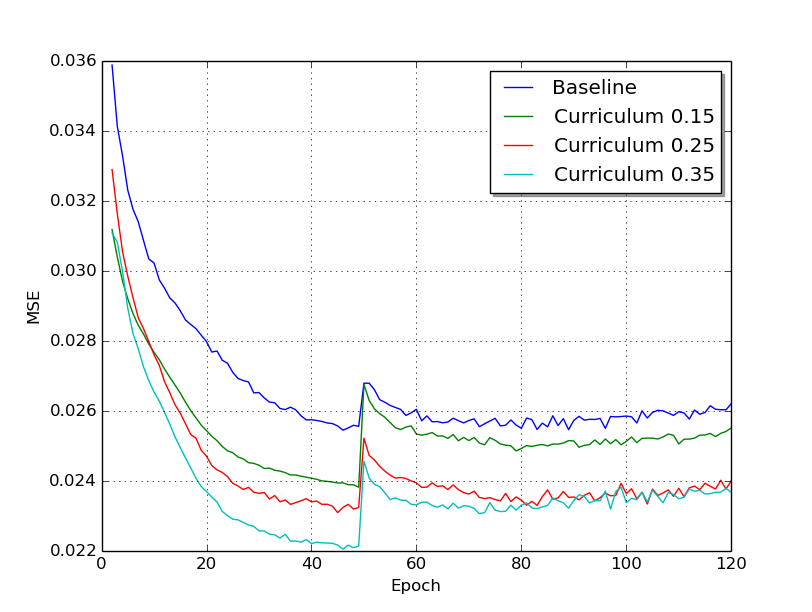
\includegraphics[width=\linewidth]{figs/E1/E1-lc.png}
\caption{Comparison of test loss} \label{fig:E1_curr_norway_loss}
\end{subfigure}
\hspace*{\fill} % separation between the subfigures
\begin{subfigure}{0.48\textwidth}
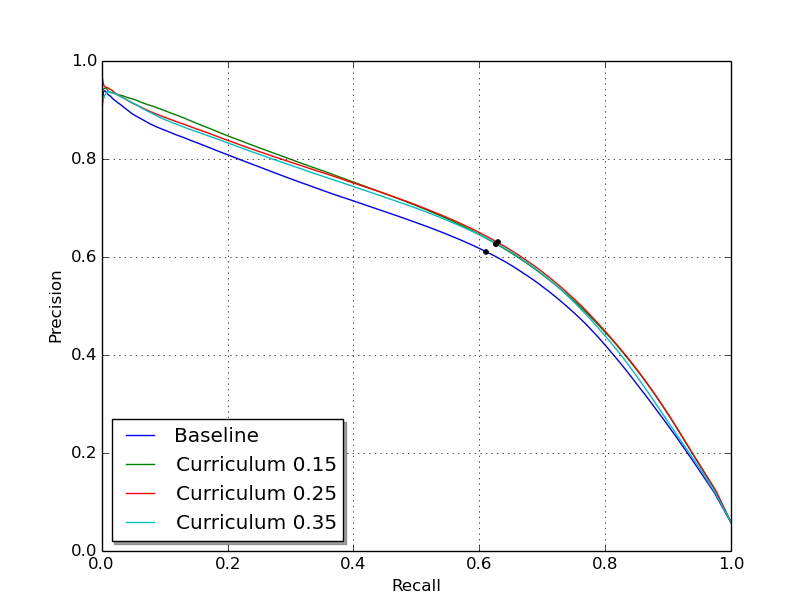
\includegraphics[width=\linewidth]{figs/E1/E1-pr.png}
\caption{Precision and recall comparisons.} \label{fig:E1_curr_norway_pr}
\end{subfigure}
\hspace*{\fill} % separation between the subfigures
\caption{E1 - Performance of curriculum learning at different thresholds, $D_{0}$ for Norwegian Roads Dataset Vbase} \label{fig:E1_curriculum_norway}
\end{figure}

In Experiment E1, the road detection system have been trained on four different patch datasets. The system's performance for each of these datasets are displayed in Figure \ref{fig:E1_curriculum_norway}. A comparison of the test loss per epoch is displayed in Figure \ref{fig:E1_curr_norway_loss}, whereas the final performance of each network is shown by a precision and recall curve in Figure \ref{fig:E1_curr_norway_pr}. The network configuration used for the tests was identical, as well as the number of training examples seen while training. The performance gap between the results, comes from the first stage of the patch datasets, where different difficulty threshold $D_0$ have been used.\\



Observing the plots in Figure \ref{fig:E1_curr_norway_loss}, the switch between stage 0 and stage 1, is clearly visible at epoch 50. The increase in test loss is most severe in the datasets formed by a curriculum strategy. Leading up epoch 50, the curriculum plots show an increasing gap in test performance against the baseline plot. After the switch the curriculum datasets still outperform the baseline dataset, even though the training set distribution of stage 1 are the same for all patch datasets.\\

Furthermore, the networks trained with a curriculum strategy shows an improved precision for all levels of recall compared to the baseline. \todo{Not so different here}\\

An interesting trend between the thresholds $D_0$ and the loss, is that decreasing the difficulty threshold, does not necessarily produce better results. The patch dataset \textit{Curriculum 0.15} has the easiest first stage, yet performs worse than \textit{Curriculum 0.25} and \textit{Curriculum 0.35} \todo{Generalize, easier examples reduce variability of training set, generalize worse. Discussion?}. \\

\todo[inline]{Need to place distribution charts somewhere}


A similar experiment was also performed on the Massachusetts Roads Dataset. In Experiment E2, networks are trained with three different patch datasets. The first stage of the baseline dataset have a first stage constructed by random sampling, which means that no examples were filtered out because of estimated difficulty. The curriculum dataset has a difficulty threshold $D_0$ of 0.25, which exclude every example with a estimated difficulty above 0.25 from the first stage. In contrast, the anti-curriculum patch dataset only have examples with a difficulty above 0.25 \todo{Mention, the non-road patches, and why non-road examples have been included}.\\


The results from this experiment can be seen in Figure \ref{fig:E2_curriculum_mass}. The switch from stage 0 and stage 1 is visible for the \textit{Baseline} and \textit{Anti-curriculum} loss plots at epoch 50. The network trained with the dataset constructed with a curriculum strategy, performs better than the baseline as seen in Figure \ref{fig:E2_curr_mass_loss} and Figure \ref{fig:E2_curr_mass_pr}. Training with an anti-curriculum strategy, where the first stage consists of harder examples, does not provide the same loss, or breakeven. This is especially evident in the plot of test loss, where the network converge around epoch 25, and start to overfit slightly towards epoch 50. From epoch 50 when stage 1 examples entered the training set, there is a dramatic decrease in test loss. The final performance of anti-curriculum learning is substantially lower than both baseline and curriculum learning, as illustrated by the breakeven points in Figure \ref{fig:E2_curr_mass_pr}.\\

The precision and recall breakeven values from Experiment E1 and Experiment E2, are listed in Table \ref{tab:results_curriculum_learning_breakeven}, and shows that training with a curriculum dataset is beneficial for both datasets.\\
\begin{figure}[!ht]
\begin{subfigure}{0.48\textwidth}
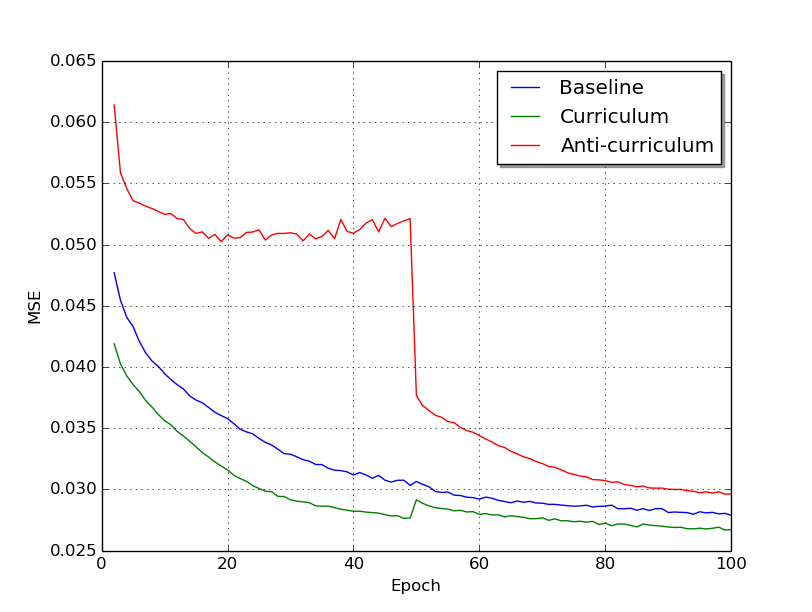
\includegraphics[width=\linewidth]{figs/E2/E2-lc.png}
\caption{Comparison of test loss} \label{fig:E2_curr_mass_loss}
\end{subfigure}
\hspace*{\fill} % separation between the subfigures
\begin{subfigure}{0.48\textwidth}
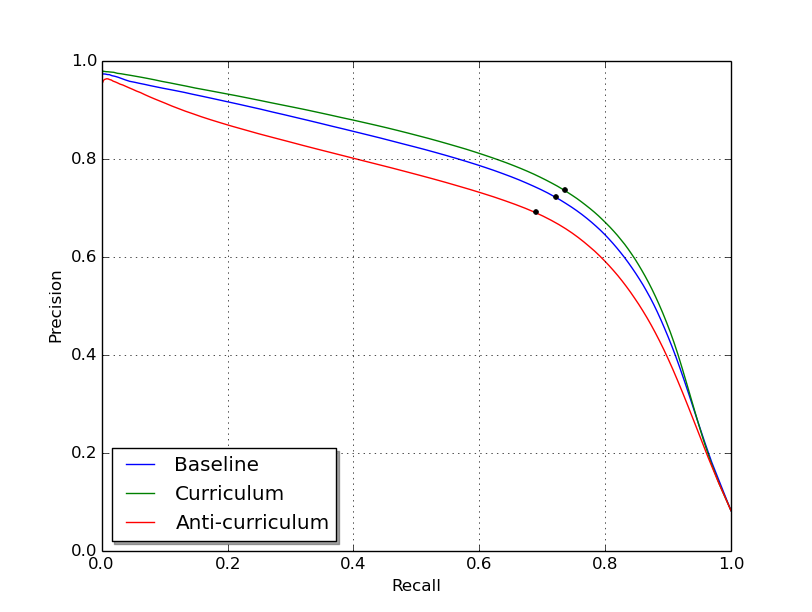
\includegraphics[width=\linewidth]{figs/E2/E2-pr.png}
\caption{Precision and recall comparisons.} \label{fig:E2_curr_mass_pr}
\end{subfigure}
\hspace*{\fill} % separation between the subfigures
\caption{E2 - Performance of curriculum learning and anti-curriculum learning for Massachusetts Roads Dataset} \label{fig:E2_curriculum_mass}
\end{figure}

\begin{table}[!ht]
\caption{Curriculum learning results.}
\begin{center}
\begin{adjustbox}{max width=\textwidth}
\begin{tabular}{+l ^l ^l ^r}\hline
\rowstyle{\bfseries}
  Experiment & $\mathbf{D_0}$ & Dataset & Breakeven\\\hline
  Baseline & 1.0 & Norwegian & 0.6105 \\
  Curriculum &0.15 & Norwegian & 0.6264 \\
  Curriculum &0.25 & Norwegian & \textbf{0.6292} \\
  Curriculum &0.35 & Norwegian & 0.6269 \\\hline
  Baseline &1.0& Massachusetts & 0.7211 \\
  Curriculum &0.25& Massachusetts & 0.\textbf{7353} \\
  Anti-curriculum &0.25 & Massachusetts & 0.6904 \\\hline
\end{tabular}
\end{adjustbox}
\end{center}
\label{tab:results_curriculum_learning_breakeven}
\end{table}

\subsection{Bootstrapping for imagery with noisy labels}
\label{sec:results_bootstrapping}

The results from comparing the bootstrapping methods and the baseline method at several levels of label noise, are displayed in Figure \ref{fig:E3_boot_mass} and Figure \ref{fig:E5_boot_norway}. The plots in the first figure are based on models trained on the Massachusetts Roads Dataset, whereas the second figure show results from training on the Norwegian Roads Dataset. The label noise have been artificially added to the label images before training. Specifically, areas of road pixels have been removed incrementally, by setting the label pixel values to zero. This process is continued until a certain percentage of road class pixels have been removed. In terms of aerial imagery, the artificially added label noise simulate omission errors, in which roads have not been marked in the label maps. Experiment E3 and E5, utilized patch datasets where 0, 10, 20 ,30 and 40 percent were removed from the labels.\\

\begin{figure}[p]
\begin{subfigure}{0.48\textwidth}
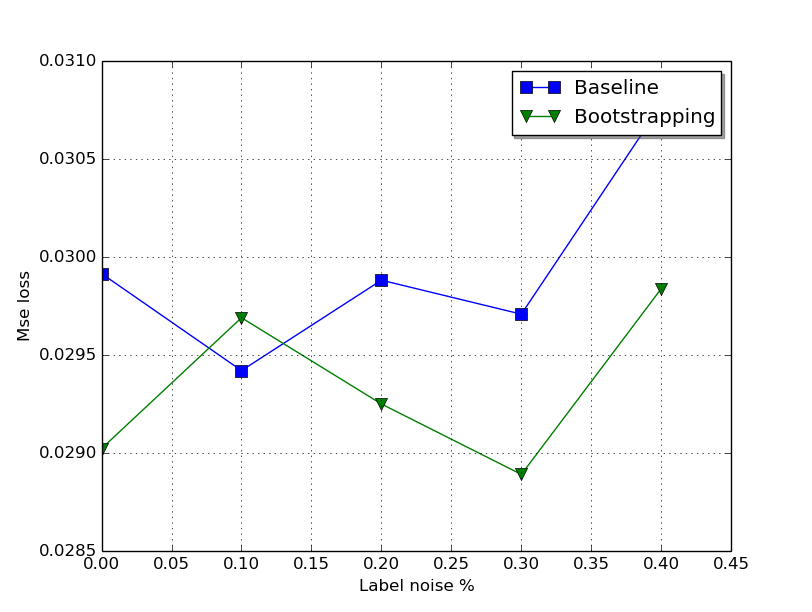
\includegraphics[width=\linewidth]{figs/E3/E3_lc_noise.png}
\caption{MSE test loss} \label{fig:E3_boot_mass_loss}
\end{subfigure}
\hspace*{\fill} % separation between the subfigures
\begin{subfigure}{0.48\textwidth}
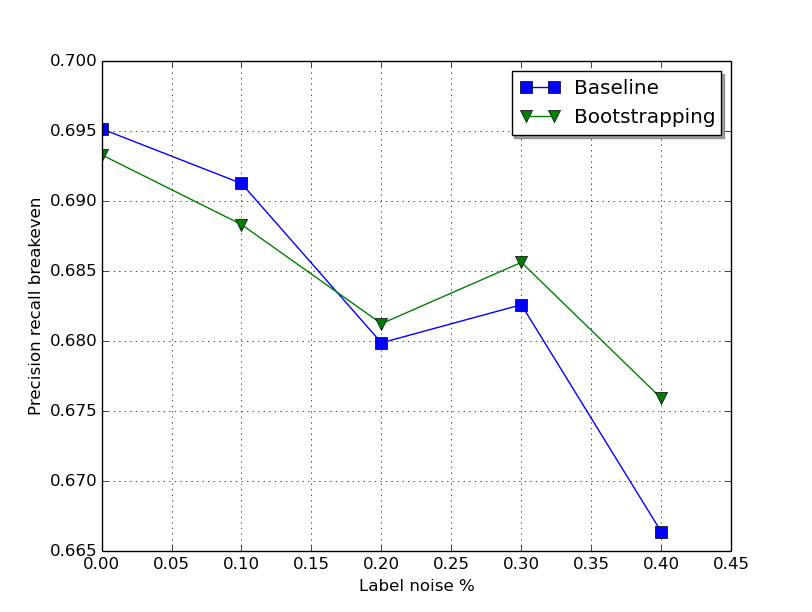
\includegraphics[width=\linewidth]{figs/E3/E3_pr_noise.png}
\caption{Precision and recall breakeven} \label{fig:E3_boot_mass_pr}
\end{subfigure}
\hspace*{\fill} % separation between the subfigures
\caption{E4 - Robustness of bootstrapping for increasing amount of label noise. Massachusetts Roads Dataset} \label{fig:E3_boot_mass}
\end{figure}

\begin{figure}[p]
\begin{subfigure}{0.48\textwidth}
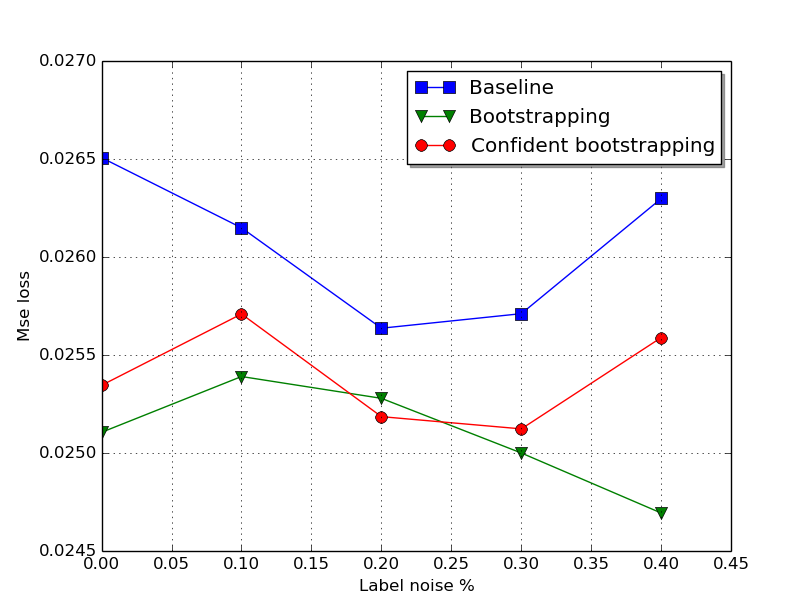
\includegraphics[width=\linewidth]{figs/E5/E5_lc_noise.png}
\caption{MSE test loss} \label{fig:E5_boot_norway_loss}
\end{subfigure}
\hspace*{\fill} % separation between the subfigures
\begin{subfigure}{0.48\textwidth}
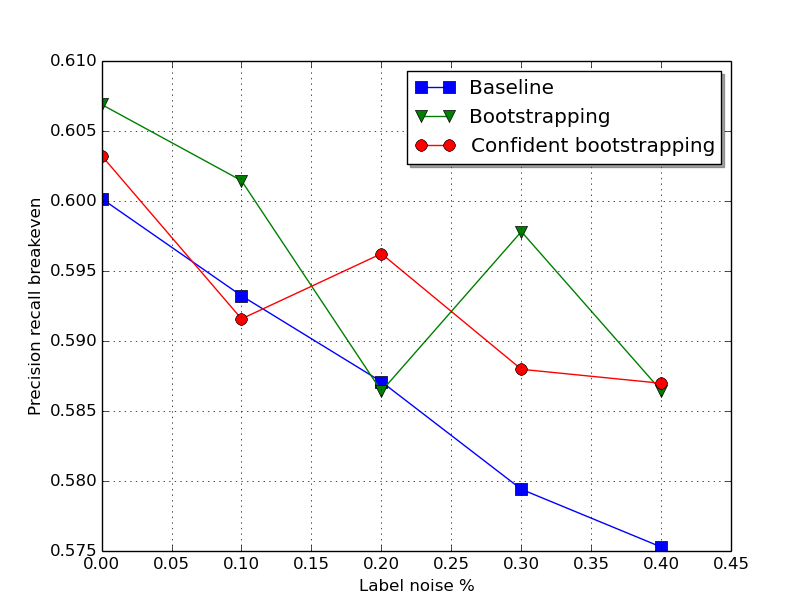
\includegraphics[width=\linewidth]{figs/E5/E5_pr_noise.png}
\caption{Precision and recall breakeven} \label{fig:E5_boot_norway_pr}
\end{subfigure}
\hspace*{\fill} % separation between the subfigures
\caption{E3 - Robustness of bootstrapping for increasing amount of label noise. Norwegian Roads Dataset} \label{fig:E5_boot_norway}
\end{figure}

In Experiment E3, conducted on the Massachusetts Roads Dataset, Figure \ref{fig:E3_boot_mass_loss} displays the averaged test loss at different levels of label noise. Generally, the baseline, which utilize the cross-entropy, seems to increase in test loss, as the noise level is increased. The bootstrapping loss function has a lower test loss for noise levels above 10 percent.\\

Figure \ref{fig:E3_boot_mass_pr}, which displays the precision and recall breakeven values at increasing levels of label noise, shows a trend of decreasing values. For label noise levels above 20 percent, bootstrapping surpass the baseline. Though, the difference in performance is limited.\\

The same type label noise experiment has been conducted for the Norwegian Roads Dataset as well, and include a plot of the confident bootstrapping performance. In Figure \ref{fig:E5_boot_norway_loss}, the test loss for bootstrapping and confident bootstrapping are consistently lower than the baseline. As expected, the precision and recall breakeven points for the baseline, decrease with increasing levels of omission noise. This can be seen in Figure \ref{fig:E4_boot_norway_vbase_pr}. Although the bootstrapping methods behave a bit more erratic, they generally tend to decrease at a slower rate \todo{A bit hard to see, doncha think!}.\\

A slightly different approach has been taken for Experiment E4. The road detection system has in this experiment been trained with a labels from the label set N50. This label set have a higher rate of omission and registration noise, than the labels in Massachusetts Roads Dataset for instance. The test set however, consists of labels originating from the Vbase label set, which is more accurate. The result from this experiment is displayed in \ref{fig:E4_boot_norway_vbase}\\

\todo[inline]{Explain what the figure shows.}

  
\begin{figure}[!ht]
\begin{subfigure}{0.48\textwidth}
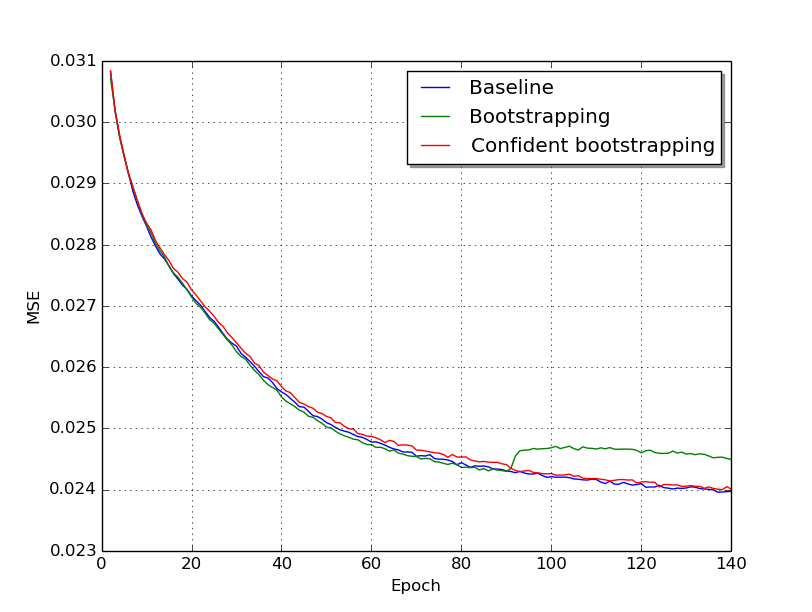
\includegraphics[width=\linewidth]{figs/E4/E4_lc.png}
\caption{MSE test loss} \label{fig:E4_boot_norway_vbase_loss}
\end{subfigure}
\hspace*{\fill} % separation between the subfigures
\begin{subfigure}{0.48\textwidth}
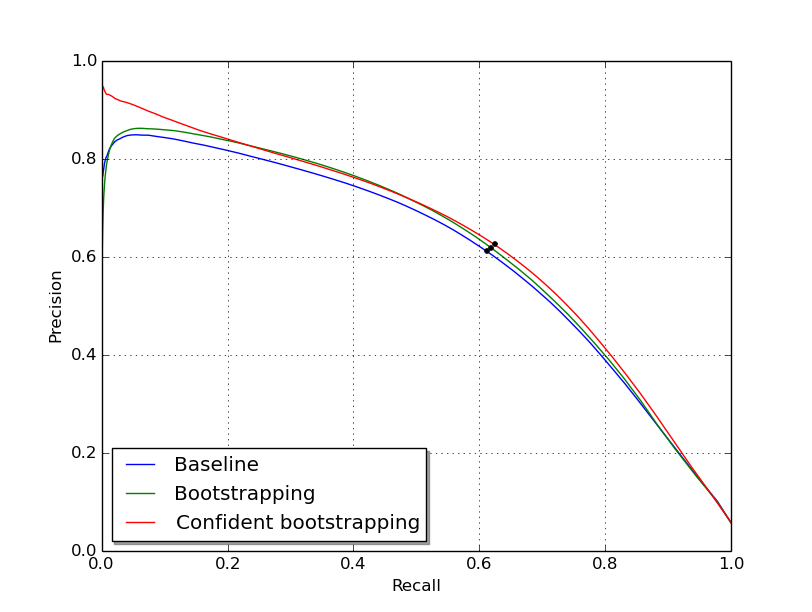
\includegraphics[width=\linewidth]{figs/E4/E4_pr.png}
\caption{Precision and recall comparison.} \label{fig:E4_boot_norway_vbase_pr}
\end{subfigure}
\hspace*{\fill} % separation between the subfigures
\caption{E4 - Comparison of loss functions for Norwegian Roads Dataset Vbase. The training set consists of labels with both registration and omission noise.} \label{fig:E4_boot_norway_vbase}
\end{figure}

\subsection{Road detection system}
\label{sec:results_road_detection_system}
Furthermore, the images in Figure \ref{fig:E6_performance} illustrate qualitatively the performance of the system. For this particular test image, the model is able to identify the majority of the roads present, except for an almost imperceptible dirt road on the right side of the image. There are also some prediction errors, such as roads being disconnected, and prediction artefacts in the forest areas. However, the majority of the forest artefacts have low prediction probabilities, and are removed when applying a threshold operation on the probabilities. The threshold value which result in the best precision and recall trade off, is used in this threshold operation.\\

An interesting observation is that the model also correctly predicts small private roads leading up to houses present in the image. Furthermore, the model detects construction roads in the upper left corner. Since these roads are not present in the label image, the model is penalized for making these predictions by the cross-entropy loss function.\\

\begin{figure}[!ht]
\begin{subfigure}{0.48\textwidth}
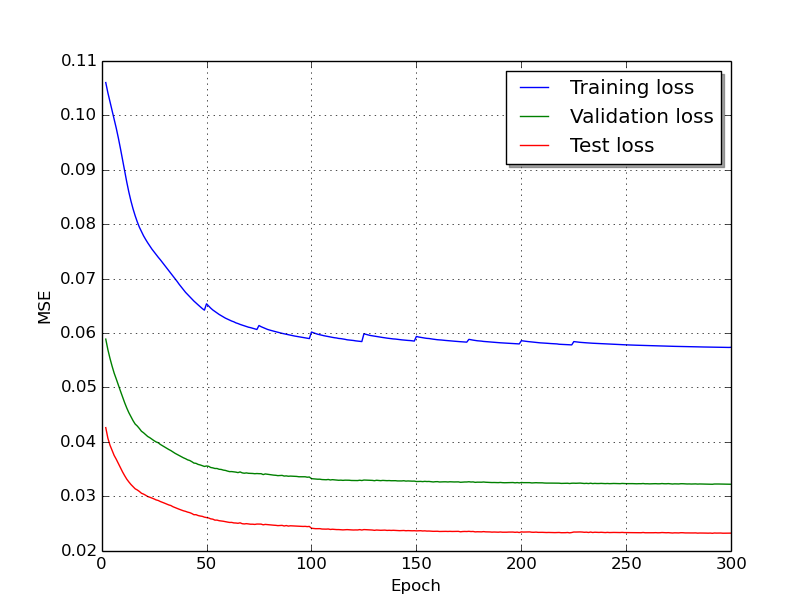
\includegraphics[width=\linewidth]{figs/E6/E6_lc_loss.png}
\caption{MSE loss} \label{fig:E6_performance_mass_lc}
\end{subfigure}
\hspace*{\fill} % separation between the subfigures
\begin{subfigure}{0.48\textwidth}
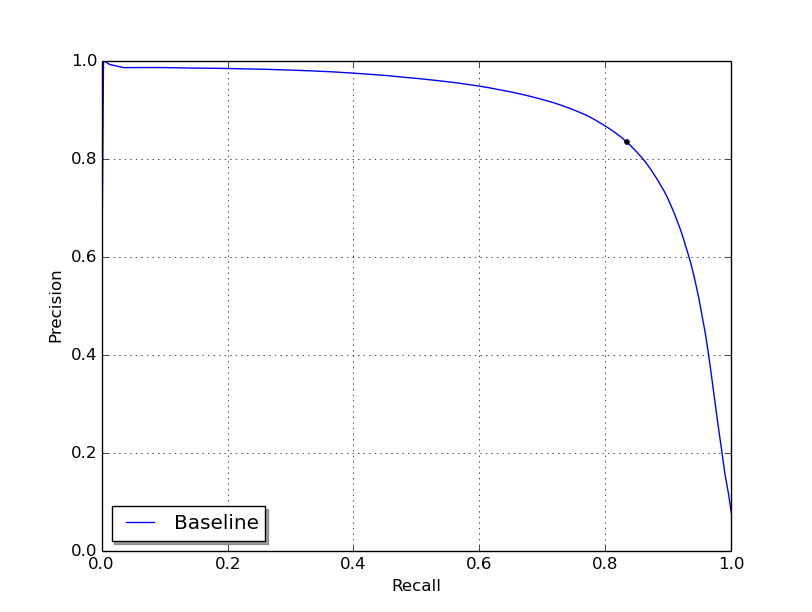
\includegraphics[width=\linewidth]{figs/E6/E6_pr.png}
\caption{Precision and recall and breakeven.} \label{fig:E6_performance_mass_pr}
\end{subfigure}
\hspace*{\fill} % separation between the subfigures
\caption{E6 - Performance of road detection system trained with Massachusetts Roads Dataset} \label{fig:E6_performance_mass}
\end{figure}

\begin{table}[!ht]
\caption{Curriculum learning results.}
\begin{center}
\begin{adjustbox}{max width=\textwidth}
\begin{tabular}{+l ^r}\hline
\rowstyle{\bfseries}
  Work & Precision and recall breakeven\\\hline
  Road detection system & 0.8341 \\
  \cite{MnihThesis} & 0.8873 \\
  \cite{saito_building_and_roads} & 0.8866 \\\hline
\end{tabular}
\end{adjustbox}
\end{center}
\label{tab:results_curriculum_learning_breakeven}
\end{table}

\begin{figure}
\begin{subfigure}{0.48\textwidth}
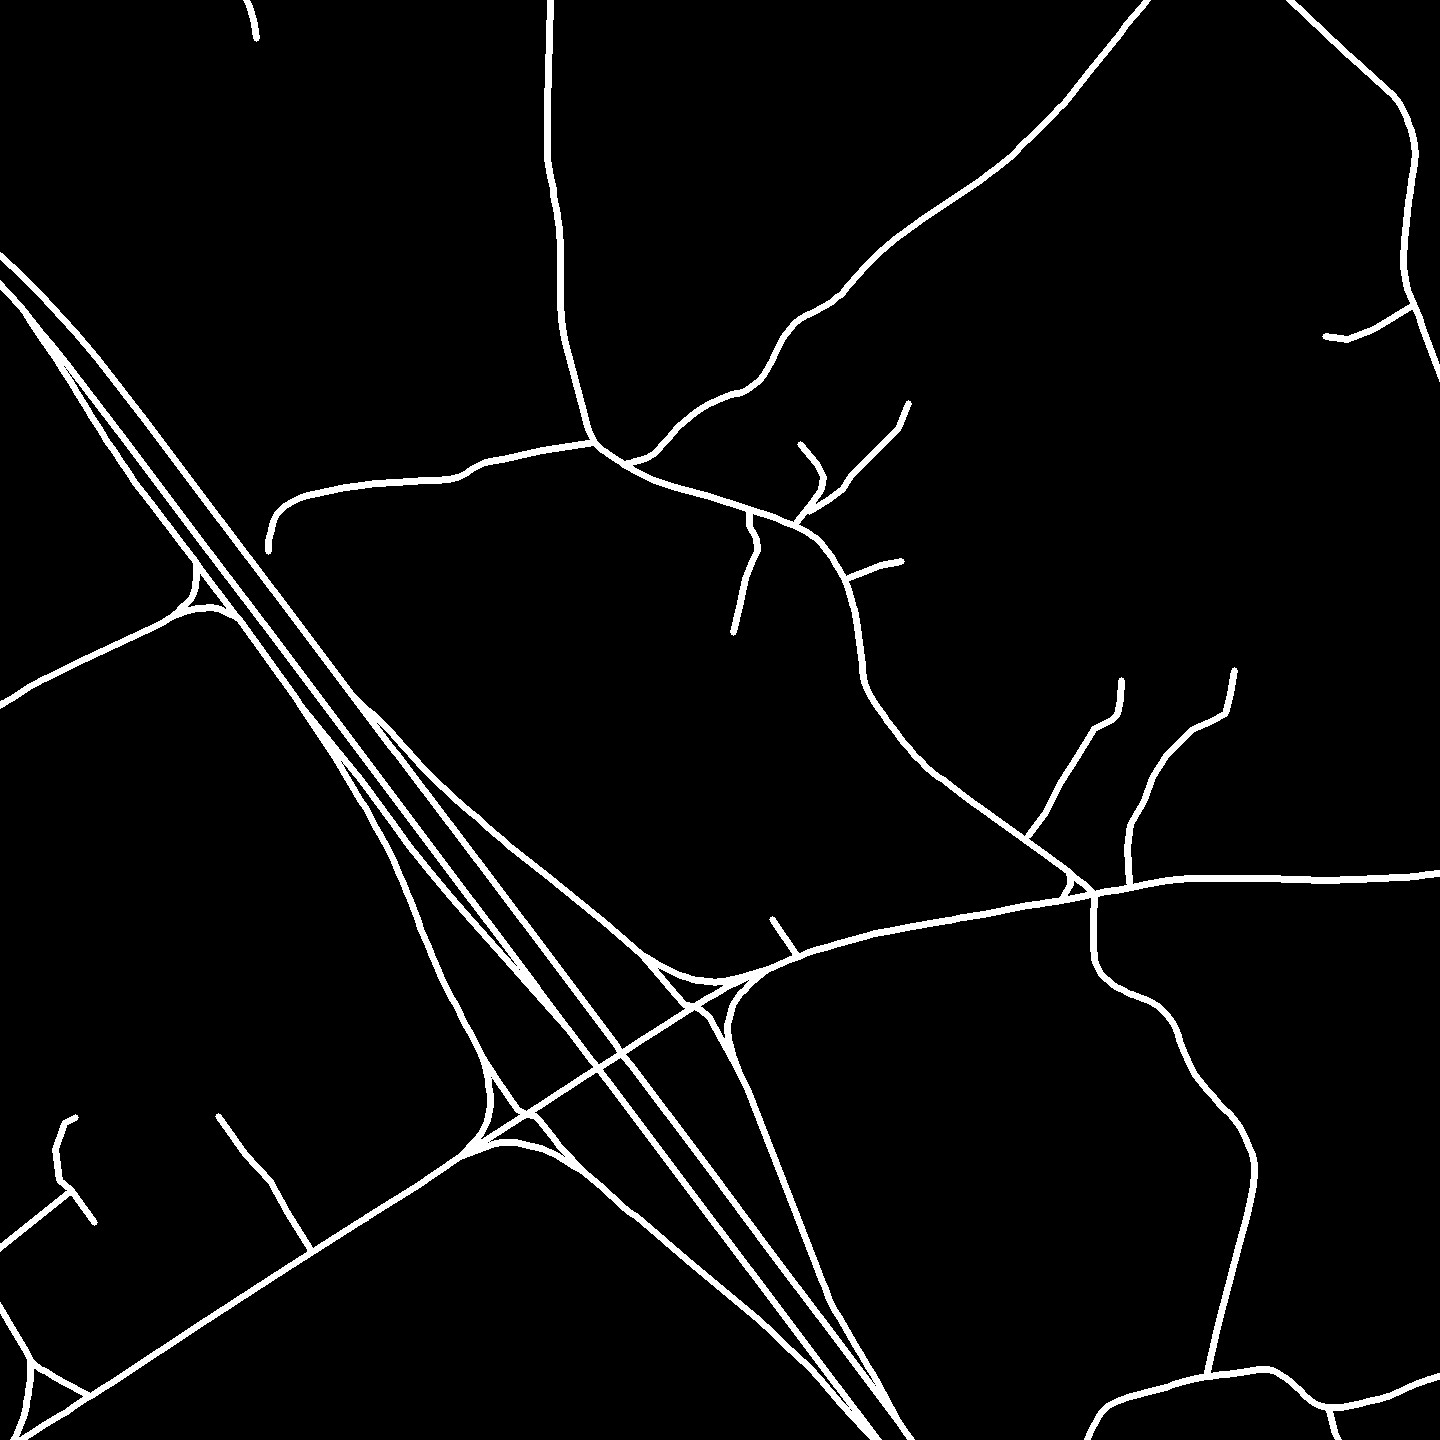
\includegraphics[width=\textwidth]{figs/E6/E6-label.jpg}
\caption{Label image.} \label{fig:E6_label_iamge}
\vspace{0.5cm} % separation vertically between the subfigures
\end{subfigure}
\hspace*{\fill} % separation between the subfigures
\begin{subfigure}{0.48\textwidth}
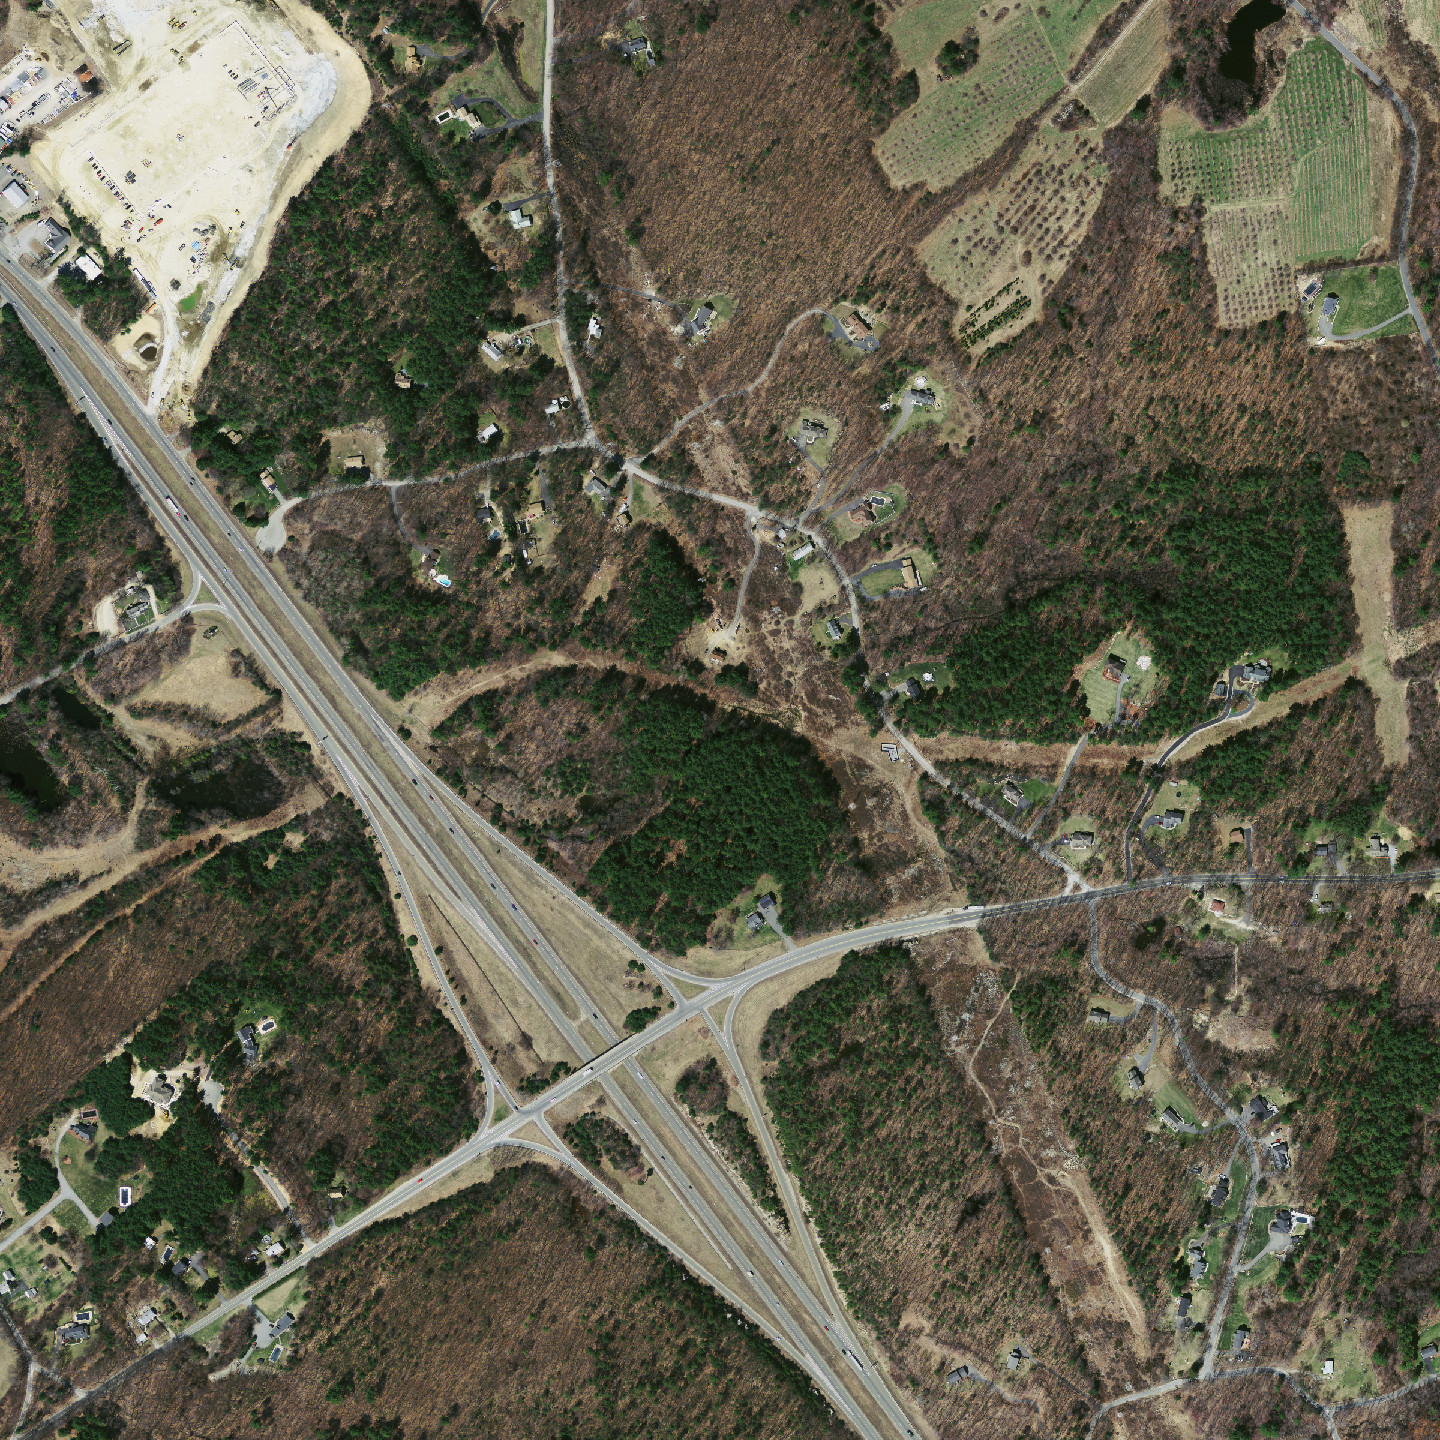
\includegraphics[width=\textwidth]{figs/E6/E6-image.jpg}
\caption{Aerial image.} \label{fig:E6_aerial_image}
\vspace{0.5cm} % separation vertically between the subfigures
\end{subfigure}

\begin{subfigure}{0.48\textwidth}
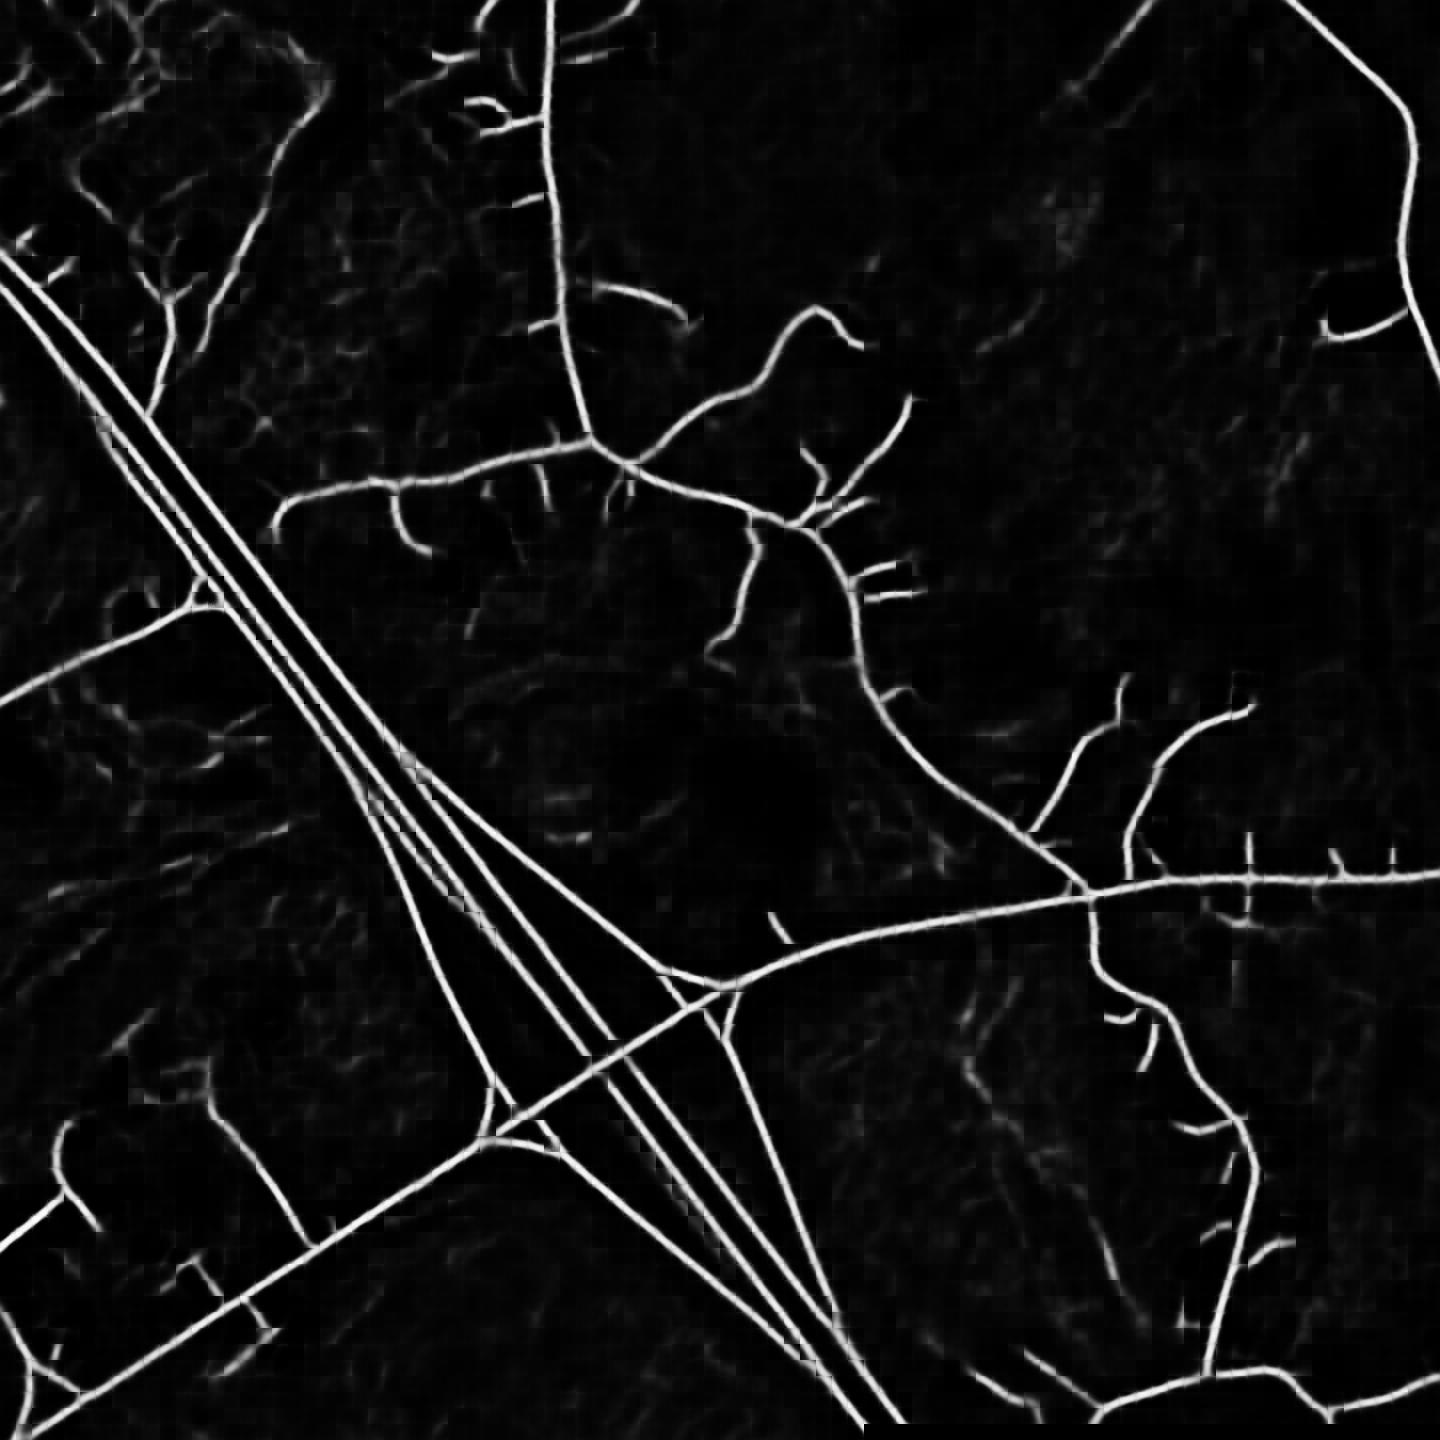
\includegraphics[width=\textwidth]{figs/E6/E6-pred.jpg}
\caption{Model predictions.} \label{fig:E6_model_predictions}
\end{subfigure}
\hspace*{\fill} % separation between the subfigures
\begin{subfigure}{0.48\textwidth}
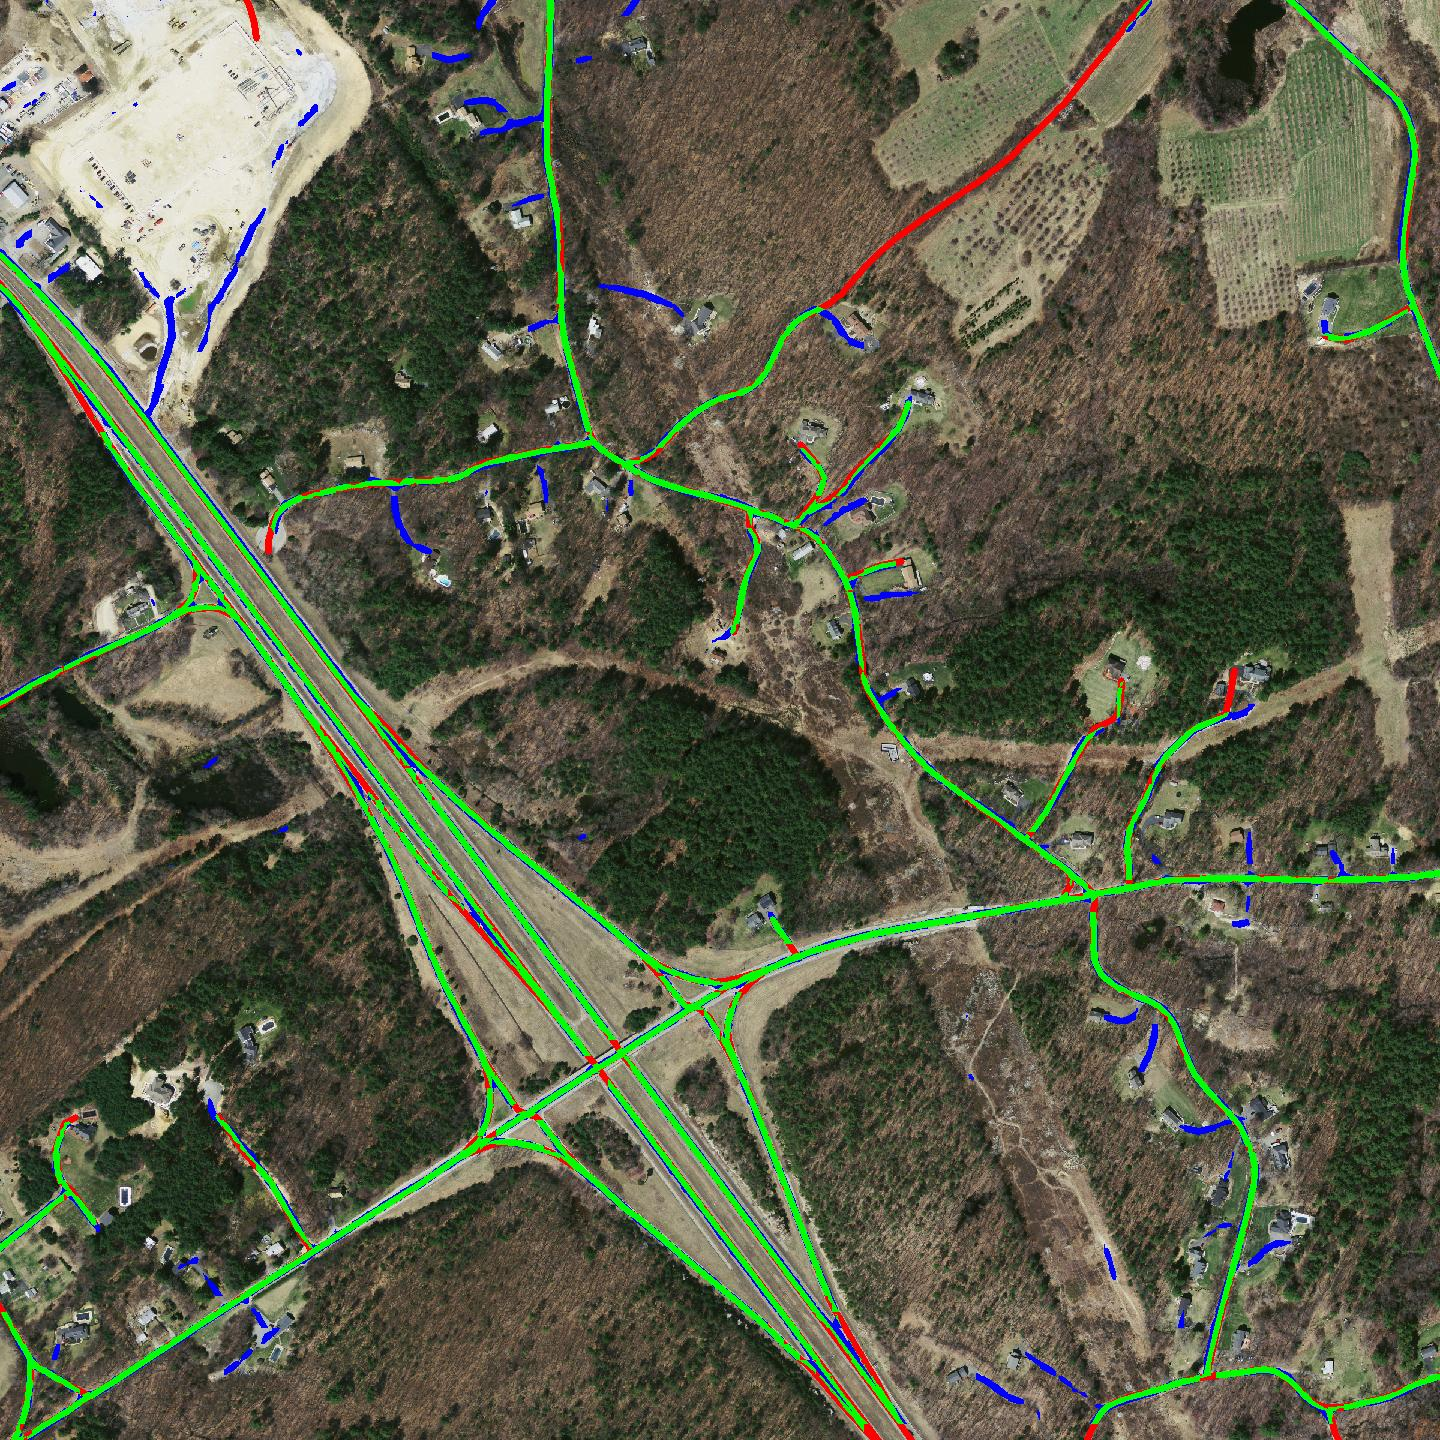
\includegraphics[width=\textwidth]{figs/E6/E6-hit.jpg}
\caption{Prediction hit and miss image.} \label{fig:E6_hit_iamge}
\end{subfigure}
\caption{E6 - Example of model's road detection performance. The aerial image is part of the test set in Massachusetts Roads Dataset} \label{fig:E6_performance}
\end{figure}




\todo[inline]{Choose what to present}
\todo[inline]{Present results for each experiment}
\todo[inline]{Avoid drawing grand conclusions. Only what your data can support}
\todo[inline]{Study tables graphs for unusual things that might raise questions with the reader}
\todo[inline]{Reason for this is the use of 50/50 split. Even though 40 percent is removed the sampling still pick out samples so that 50 percent of patches contain road class pixels. In discussion?}

\section{Experimental Analysis}
\label{sec:Discussion}
In the following analysis, the results presented in the previous section will be explored more in-depth. Furthermore, qualitative results from the road detection system are evaluated, and might illustrate why methods for dealing with noisy labels are important for this type of dataset.\\

The \ac{CNN} and the proposed methods are in some sense comparable to the three groups of approaches for dealing with label noise, described in Section \ref{sec:background_label_noise}. The bootstrapping loss function is clearly a noise-tolerant approach, where the loss function is modified in an attempt to make the network more robust towards label noise. The \ac{CNN} and the regularization methods can be categorized as a noise-robust model. Whereas, curriculum learning in some sense can be described as a data cleansing method. The ``simple" stages are created based on filtering techniques, where inconsistency between label and prediction determines whether an example is excluded or not. However, examples are not excluded or relabeled from every stage, but only from the initial stages of training.\\

\subsection{The Effect of Bootstrapping}
Unfortunately, the effect of employing the bootstrapping loss function is quite small. However, the bootstrapping methods did perform nearly equal or slightly better when observing the breakeven values in Experiment E1, E2, and E3, and for increasing levels of omission noise,  as seen in Figure \ref{fig:E1_boot_mass} and Figure \ref{fig:E2_boot_norway}. It seems that bootstrapping do exhibit some robustness towards label noise. Compared to the performance of the baseline, the difference in both test loss and breakeven seems to be increasing.  \\

Even though up to 40\% of the roads present in the label images were removed, it did not particularly affect the baseline much. The baseline network seems to be surprisingly robust towards label noise. However, the default patch dataset sampling policy might be somewhat responsible for this.\\

In Experiment E1, and E2, only omission noise was artificially added to the label images. This simply removed road pixels from the label images, until a certain percentage of road pixels had been removed. However, when the patch creator sampled the aerial dataset, the preference for an even balance between patches containing road pixels and patches not containing any road pixels were enabled. Even for increasing levels of omission noise, the patch creator still sampled around 50\% road patches with almost no noise added. The portion of non-road patches in the patch dataset was of course affected by the increase in label noise. Adding artificial, but realistic registration noise to the label images were not done in the experiments. This would have affected the entire patch dataset. In Appendix \ref{app:randomnoiseexperiment}, the results from increasing levels of label noise by flipping label pixels are presented. In this scenario, bootstrapping is much more effective. Unfortunately, this type of label noise is highly unrealistic for this type of dataset.\\

There is also the issue of seemingly contradictory results in Experiment E3. Even though bootstrapping in Figure \ref{fig:E3_boot_norway_vbase} shows an increase in the loss towards the end, it still achieves a better precision and recall curve than the cross-entropy loss. This is probably an indication of bootstrapping actually working. It seems that the bootstrapping loss function slightly adjusts the predictions to be more consistent between perceptually similar examples at the cost of an increasing test loss. The Vbase test set labels are not perfect, and exhibit some registration and omission noise, which probably explains the increase in test loss. The bootstrapping function might be reducing the impact of local registration noise by adjusting the predictions to fit the road pixels better. These prediction adjustments will be visible in the test loss plot, but will not affect the precision and recall curve because of the relaxed measure of precision. \\

The alternative bootstrapping loss function behaves slightly different compared to bootstrapping, as demonstrated by the test loss figures \ref{fig:E2_boot_norway_loss}, and \ref{fig:E3_boot_norway_vbase_loss}. In these figures, the confident bootstrapping seems to follow the general outline of the baseline more closely than bootstrapping. The only difference between the two loss functions is that confident bootstrapping modifies targets using only confident pixel predictions. In addition, for the N50 label set in Experiment E3, this loss function actually performed slightly better than bootstrapping and the baseline in terms of precision and recall. \\ 

In summary, the experiments show that bootstrapping has a small positive effect on the results. However, the performance gains were not statistically significant for tests that involved omission and registration noise.\\

%An additional challenge was the constraint on runtime. To run 10 replicate experiments, the patch dataset size had to be limited. This might impact the performance of the bootstrapping methods, since they rely on models that have already incorporated some implicit knowledge about the data.\\

\subsection{Curriculum Learning by Using an Artificial Teacher}

All experiments comparing a randomly sampled patch dataset and a patch dataset constructed from a curriculum strategy, showed that presenting easier examples first have a positive impact on the classifier's ability to generalize. Furthermore, the proposed curriculum strategy that is based on measuring disagreement between the labels and the predictions that were produced by a teacher classifier, seems to be a viable approach for conducting curriculum learning.\\

A benefit of using this particular curriculum strategy is that it appears to be generally applicable. As long as a teacher classifier is trained to a certain level for an arbitrary dataset, it should be possible to create a curriculum dataset using the difficulty estimator $d(y,q)$. However, it does require training an additional classifier, and the resulting quality of the curriculum dataset probably corresponds to the competency of the teacher classifier. For images this strategy is compelling, since judging the perceived difficulty of examples based on the actual image content is hard.\\

Experiment E4 and E5 demonstrated that the examples presented first do impact the final performance of the network. This is evident from both the precision and recall curve, as well as the test loss. It is conceivable that a less challenging training set distribution puts the network in an advantageous area of parameter space. Even though the latter half of training for the curriculum tests were conducted on a training set with the same example distribution as the baseline tests, the starting advantage of curriculum learning was still preserved in the final performance.  \\

From Experiment E4 it is also clear that anti-curriculum learning does not provide the same advantage as curriculum learning. The performance in Figure \ref{fig:E4_curr_mass_loss} converges already at around epoch 25, with a test loss considerably higher than the baseline. It is only able to approach the test loss of the baseline after switching to the natural example distribution at epoch 50. The final test loss converged to a level well above the baseline. This also illustrates that the examples presented first have a large influence on the outcome. It is possible that early optimization on harder examples can guide the network to an unfavorable local minimum, which is hard to escape from later on.\\

The results further show that the outcome of curriculum learning is sensitive to the threshold parameter $D_0$. Figure \ref{fig:E5_curr_norway_loss} reveals that decreasing threshold value $D_0$ diminishes the effect of curriculum learning. Decreasing the threshold value results in a smaller pool of eligible examples that can be included in the first stage of a training set, which, in turn, can reduce the training set variability.\\ 

A bit surprising are the results from Experiment E6, which showed that training with the first stage only, did better than curriculum learning. This indicates that the inexperienced teacher model actually did a good job separating  the very hard and possibly inconsistent examples out from the first stage. It also shows that the second stage probably contained a good amount of inconsistent examples, which can penalize the network incorrectly and affect the outcome. Alternatively, this might indicate that the threshold parameter $D_0$ was set to a value which resulted in sufficient example variation in the first stage training set. The network is therefore able to generalize well to the task of road detection.\\

However, assuming that harder examples are inconsistent and exclude them entirely from the training set should be done with caution. This could lead to hard, but correctly labeled examples being excluded, as well as unfamiliar examples that the curriculum teacher has not seen before. If the teacher classifier could accurately detect inconsistent labeling, there would be no reason for doing curriculum learning in the first place.\\ 

A potential reason for the large spike in test loss after a stage switch is that the entire training set is suddenly replaced. As seen in the test loss of Figure \ref{fig:E6_gradual_loss}, gradually mixing in examples from smaller subsequent stages seems to alleviate this. The breakeven point for this test is also substantially higher than that of the baseline, the first-stage-only curriculum, and the inexperienced teacher classifier.\\

In summary, the composition of the first stage has a considerable effect on the outcome of training. Furthermore, the results demonstrate that the proposed curriculum strategy works well in practice.

\subsection{Performance of the Road Detection System}
The images in Figure \ref{fig:E7_performance} illustrate qualitatively the performance of the network with the best performance on the Massachusetts Roads Dataset. The prediction image in Figure \ref{fig:E7_model_predictions} has been stitched together from $16 \times 16$ prediction patches. For this particular test image, the model was able to identify the majority of the roads present, except for an almost imperceptible dirt road on the right side of the image. There are also some prediction errors, such as roads being disconnected, and prediction artifacts in the forest areas. However, the majority of the forest artifacts have low prediction probabilities, and can be removed by a threshold operation applied to the probabilities. For instance, the threshold value which results in the best precision and recall trade-off of the model was used to binarize the predictions in Figure \ref{fig:E7_hit_image}.\\

An interesting observation is that the model also correctly predicts small private roads leading up to houses, as seen in Figure \ref{fig:E7_performance}. Furthermore, the model detects construction roads in the upper left corner. Since these roads are not present in the label image, the model is penalized for making these predictions by the cross-entropy loss function.\\

The prediction errors are displayed in Figure \ref{fig:E7_hit_image}, where the road label pixels and road prediction pixels are superimposed on the aerial image. The road pixels that are colored green have been correctly predicted, whereas the red and blue colored pixels show the prediction errors. The red pixels indicate areas where the system failed to predict road, and the blue pixels show areas where the system incorrectly predicted road. Yet, the majority of the prediction errors are understandable, and arguably not actually errors at all. Most of the blue areas are covering pixels that depict asphalt surfaces, and some of the red areas have trees covering the road. However, a certain challenge is the amount of disconnected roads, that especially occur at road junctions and highway ramps. Possible reasons for these prediction errors can be the low frequency of junctions and ramps in the dataset, or that the model capacity is inadequate. More results similar to Figure \ref{fig:E7_performance} can be found in Appendix \ref{app:roaddetectionresults}.\\



\begin{figure}
\begin{subfigure}{0.48\textwidth}
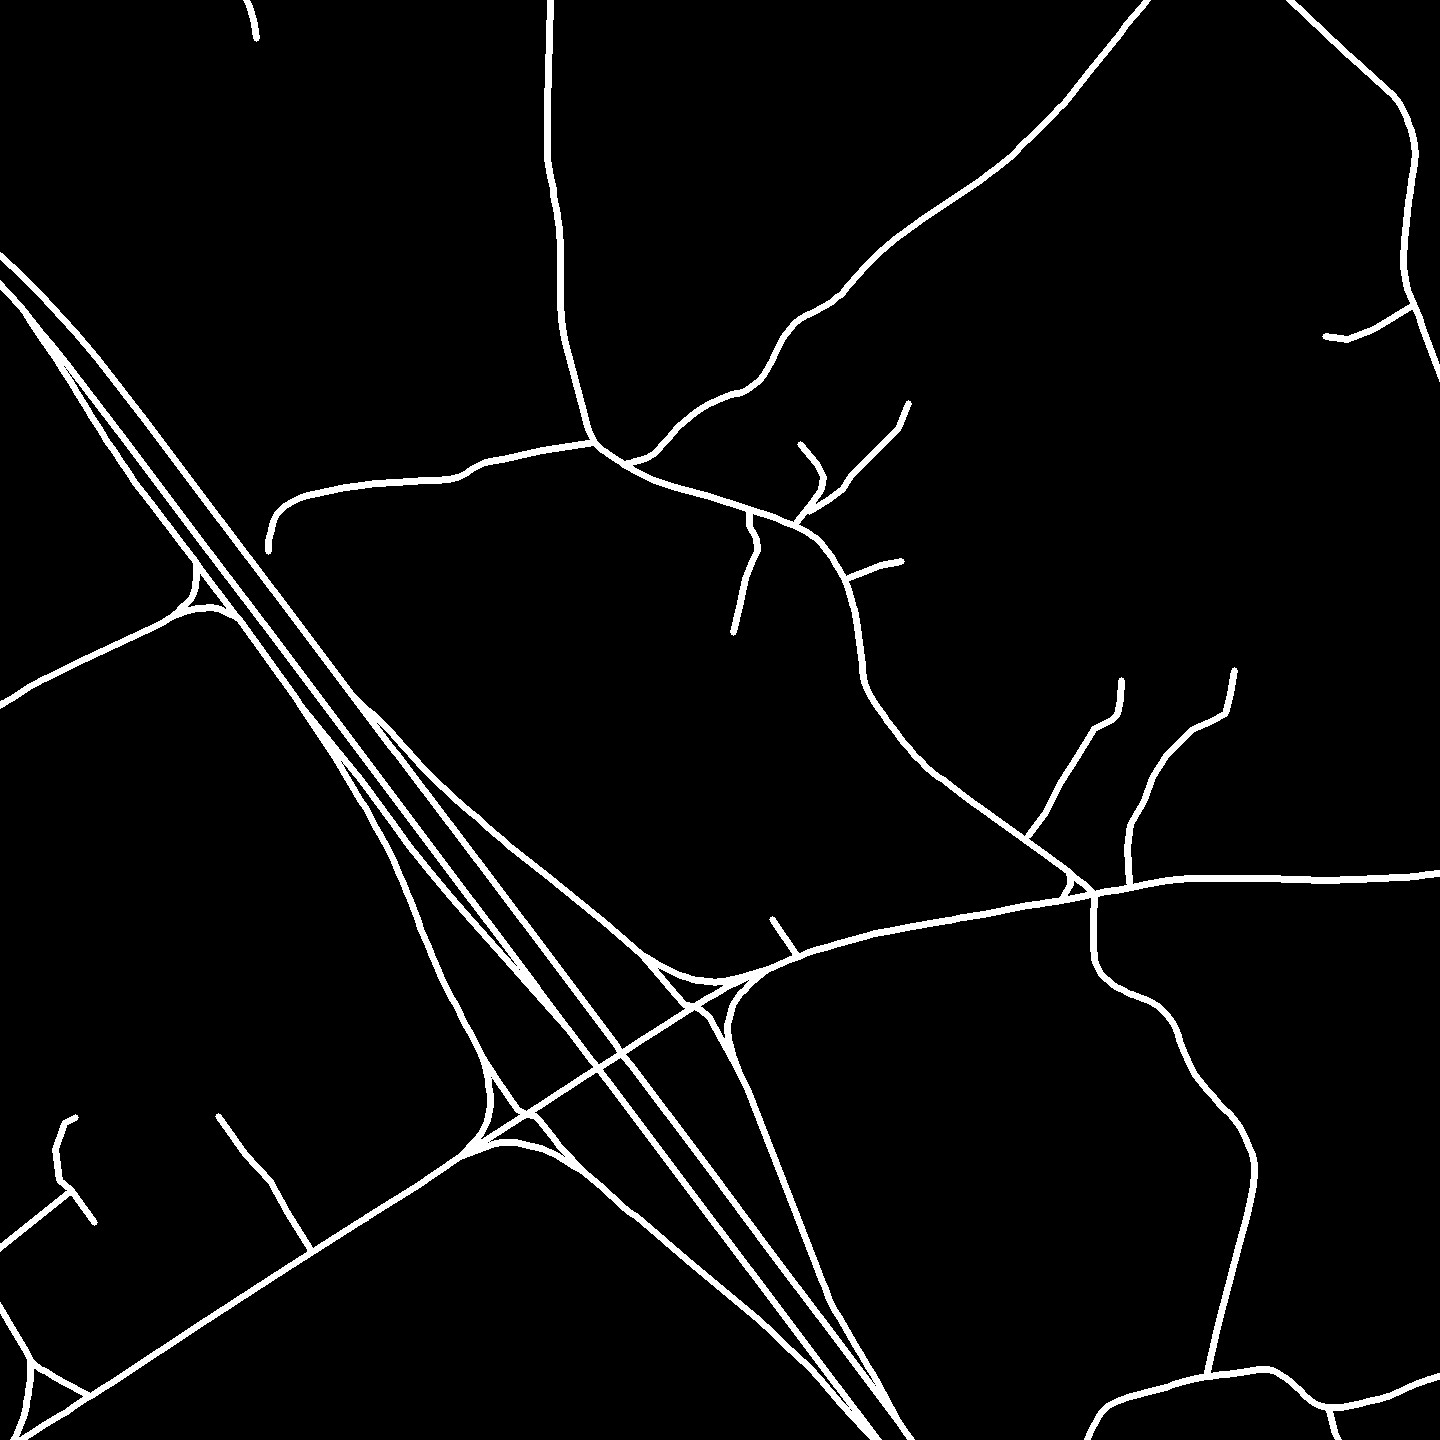
\includegraphics[width=\textwidth]{figs/E7/E7-label.jpg}
\caption{Label image.} \label{fig:E7_label_iamge}
\vspace{0.5cm} % separation vertically between the subfigures
\end{subfigure}
\hspace*{\fill} % separation between the subfigures
\begin{subfigure}{0.48\textwidth}
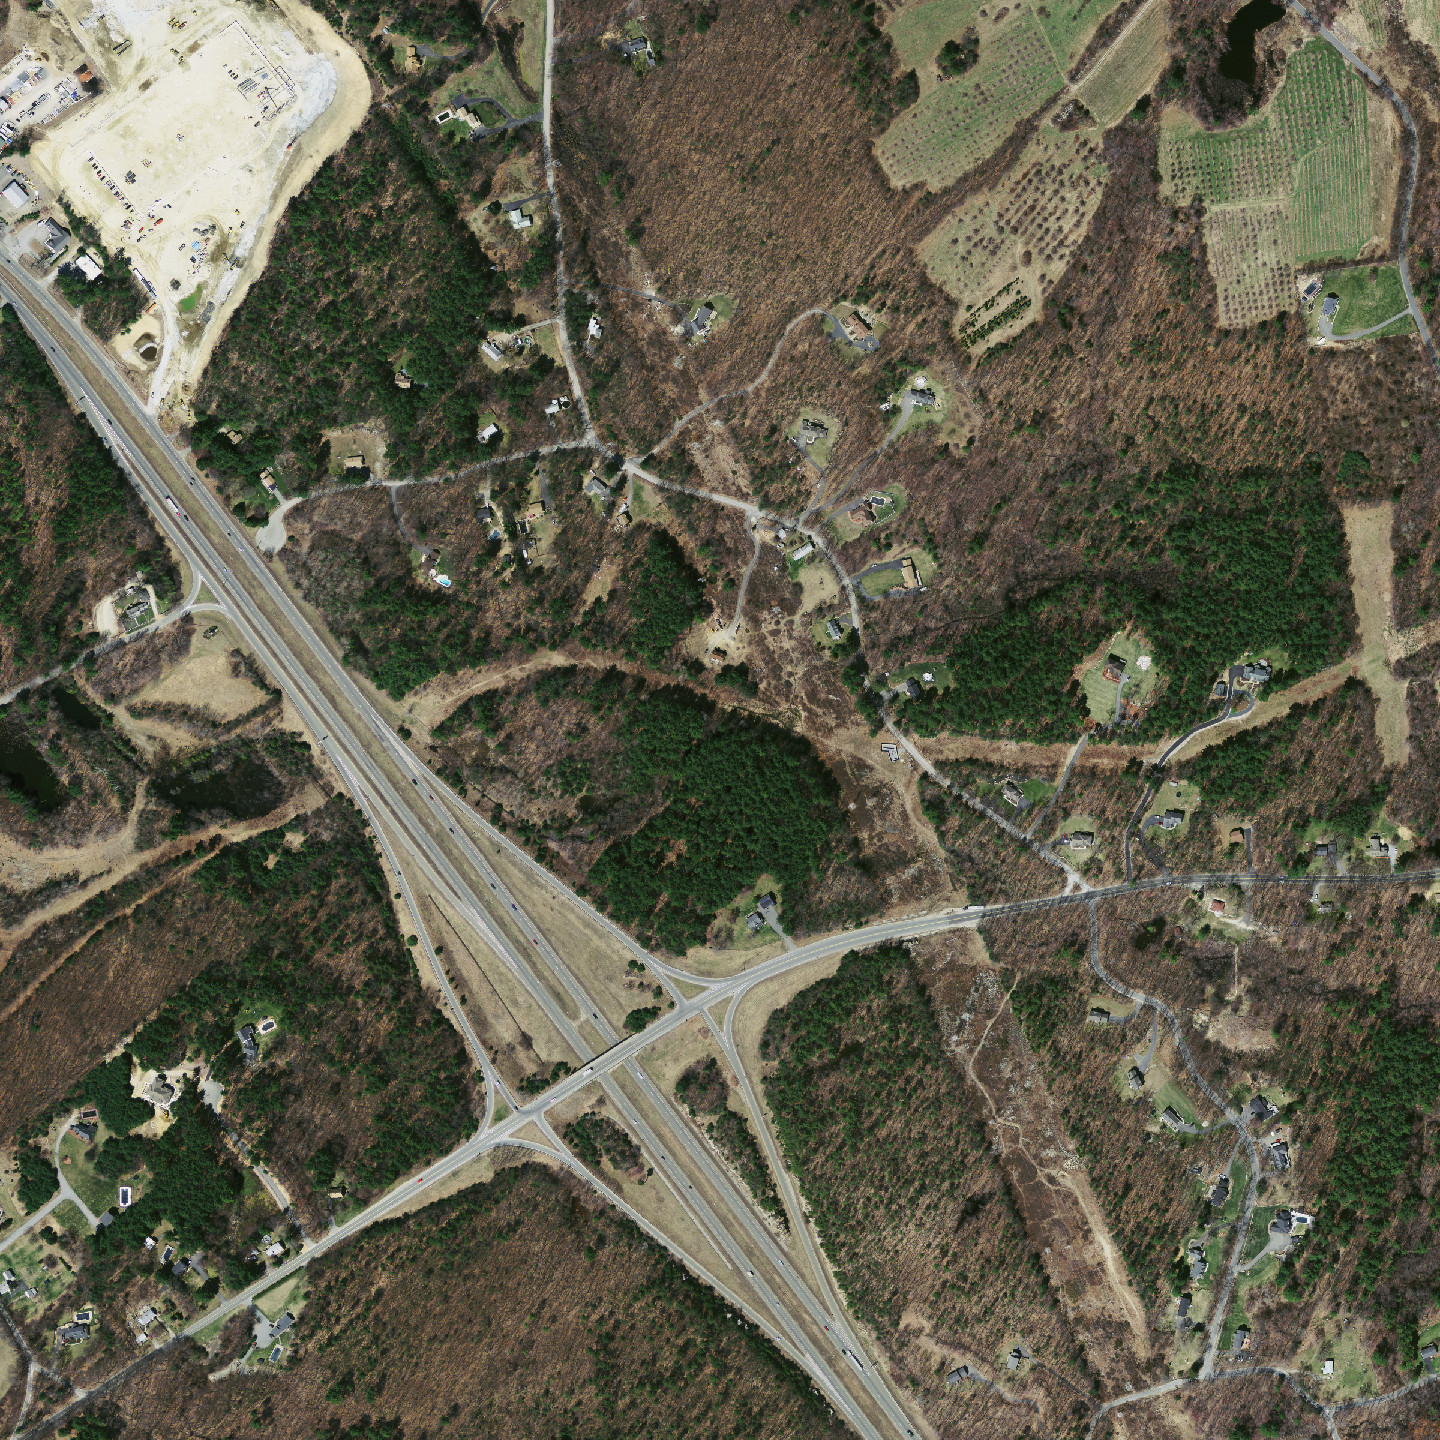
\includegraphics[width=\textwidth]{figs/E7/E7-image.jpg}
\caption{Aerial image.} \label{fig:E7_aerial_image}
\vspace{0.5cm} % separation vertically between the subfigures
\end{subfigure}

\begin{subfigure}{0.48\textwidth}
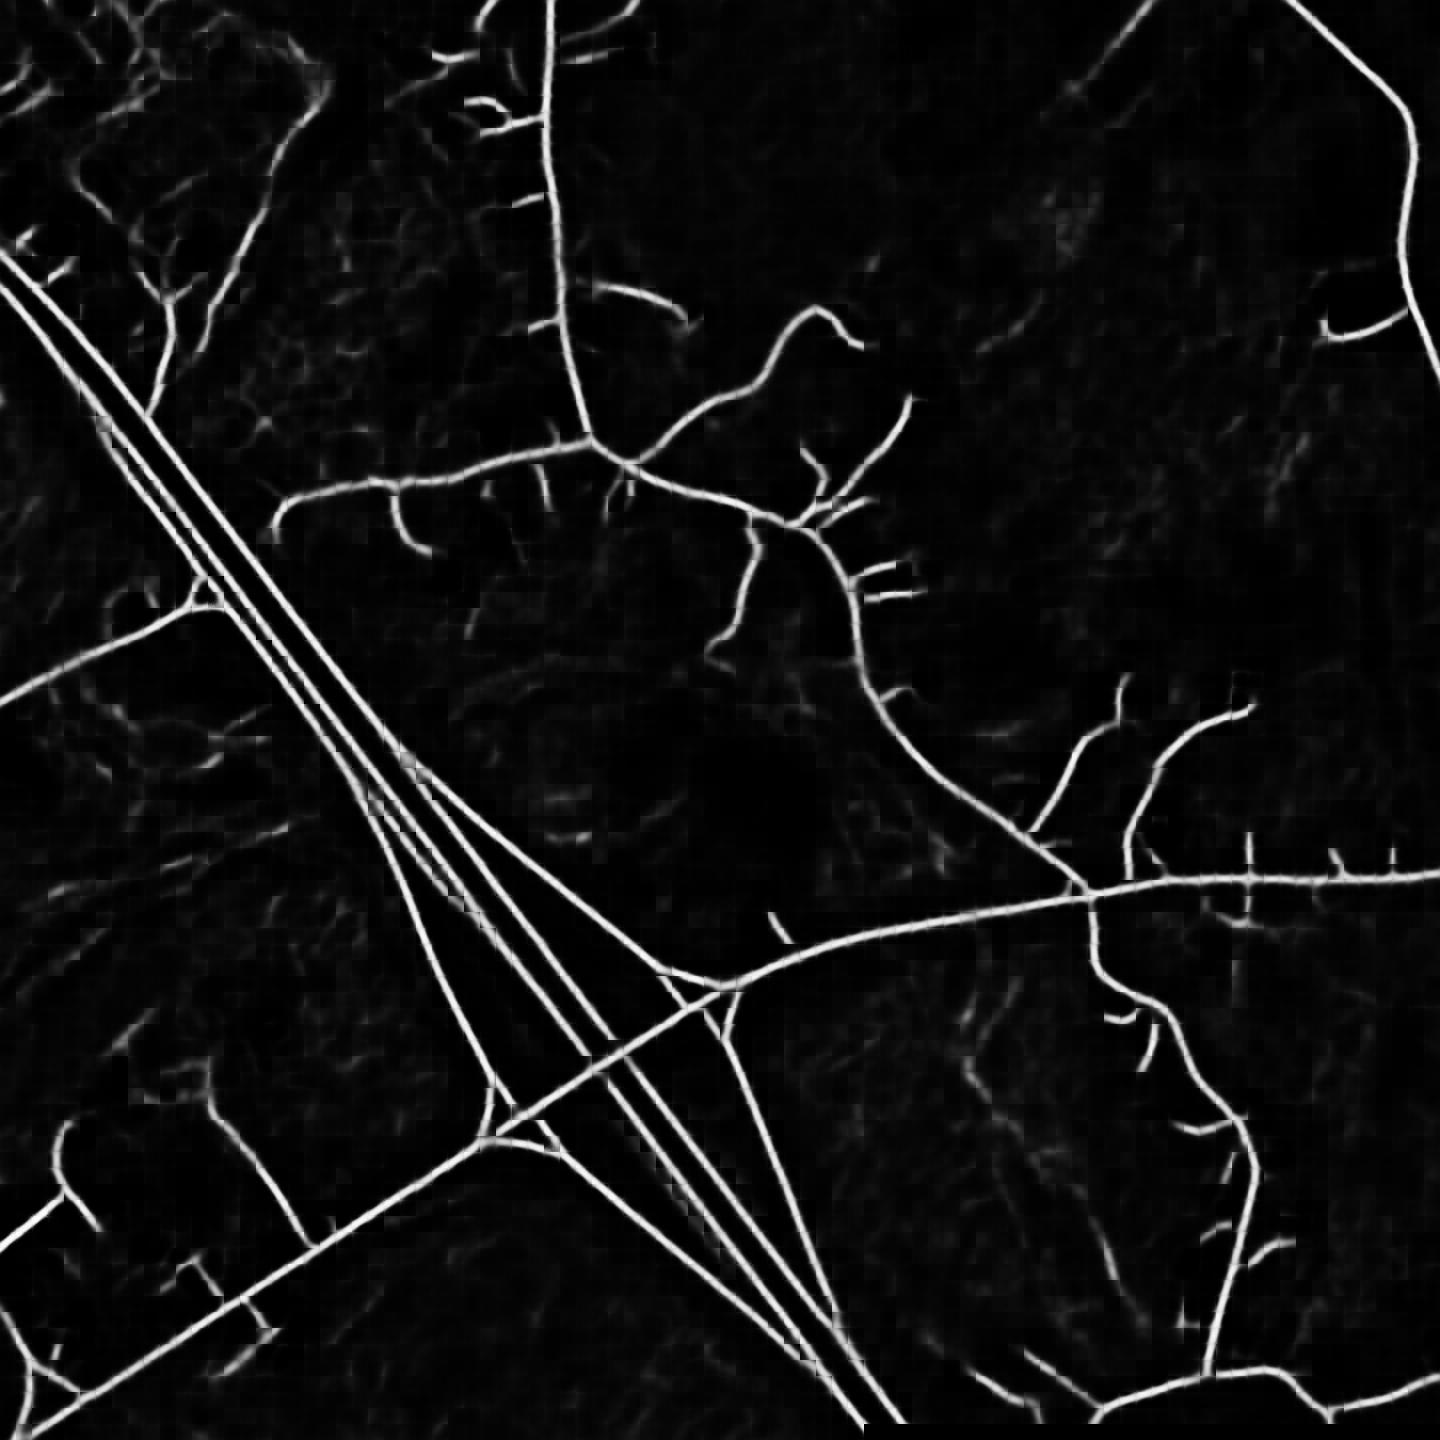
\includegraphics[width=\textwidth]{figs/E7/E7-pred.jpg}
\caption{Model predictions.} \label{fig:E7_model_predictions}
\end{subfigure}
\hspace*{\fill} % separation between the subfigures
\begin{subfigure}{0.48\textwidth}
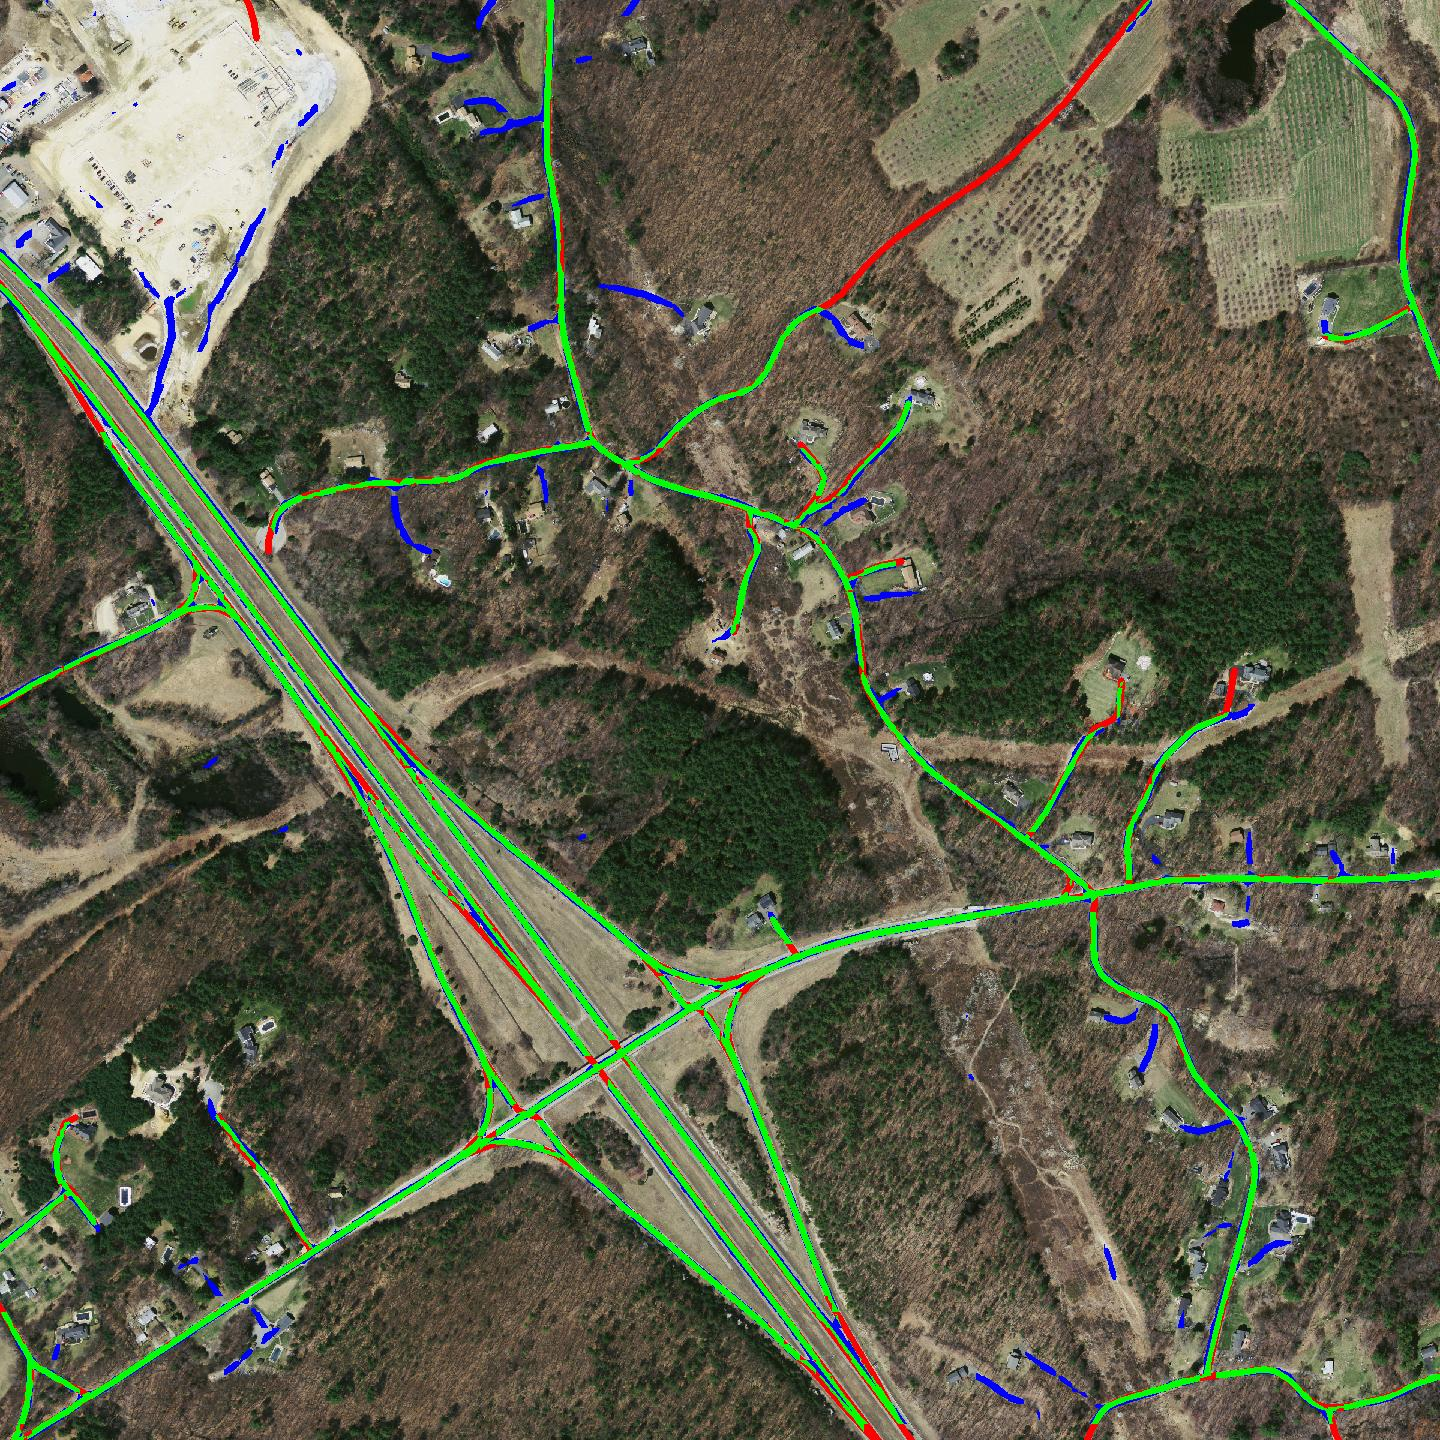
\includegraphics[width=\textwidth]{figs/E7/E7-hit.jpg}
\caption{Prediction hit and miss image.} \label{fig:E7_hit_image}
\end{subfigure}
\caption[E7 - Qualitiative results of the road extraction system ]{E7 - Example of model's road detection performance. The aerial image is part of the test set in the Massachusetts Roads Dataset.} \label{fig:E7_performance}
\end{figure}

One of the most compelling ways of reducing the number of disconnected roads is by utilizing structured output prediction methods, as discussed in Section \ref{sec:related_works}. Several studies \citep{Kluckner_semantic_height} \citep{LeCun_semantic} \citep{Mnih_roads_high_res_aerial_images} have shown that employing a smoothness prior by taking neighboring predictions into account can significantly improve generalization in semantic segmentation tasks. This is unfortunately outside the scope of this thesis.\\

The precision and recall breakeven point of M1 is considerably lower compared to other works, as seen in Table \ref{tab:results_road_detection_breakeven}. The most likely explanation is the default configuration of this network. The configuration of the first layer in the network trained by \citep{MnihThesis} was different. \citep{MnihThesis} used overlapping max pooling in the first layer, whereas the max pooling of M1 was non-overlapping. This resulted in fewer learnable parameters in M1, which could have affected the network's model capacity or ability to fit the data. The spatial reduction of the input in the first convolutional layer especially affects the number of incoming connections to the first fully connected layer of the network.  The network by \cite{MnihThesis} has approximately 17.3 million adjustable weights.\\

This was tested in Network M2, which used a different stride and kernel sizing. The number of adjustable weights in this network was around 5 million compared to around 1.6 million in Network M1. A large portion of the difference can be traced back to the massive increase in incoming connections to the fourth layer. The number of incoming connections in M1 was 80, compared to 720 in M2. This network achieved a precision and recall breakeven point of 0.8494, even though it was trained for fewer epochs, and with a smaller training set. In addition, this network was trained using a gradual curriculum strategy, and used the confident bootstrapping loss function. \\

The same network configuration, loss function, and training regime were tested with the Norwegian Roads Dataset Vbase in Network N1. The precision and recall breakeven point of this network was substantially lower. There are probably several reasons for this. First, the lower \ac{GSD} of this dataset implies that image  patches of $64 \times 64$ pixels convey less context compared to similarly sized patches from the Massachusetts Roads Dataset. This might reduce the network's ability to discriminate between road and non-road pixels in situations where surrounding context is key. Second, the results from the two roads datasets cannot be directly compared because they are different. The Norwegian Roads Dataset has images of varying image quality, and depict a wide range of topographical features. Furthermore, The Vbase label set has been rasterized with ill-suited line thicknesses for roads that are particularly wide or narrow. The examples in Figure \ref{fig:ill-suited} illustrate this. 

\begin{figure}
\begin{subfigure}{0.28\textwidth}
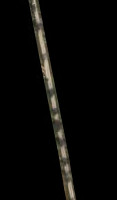
\includegraphics[width=0.73\textwidth]{figs/illsuited_label.jpg}
\caption{Non-road pixels superimposed.} \label{fig:ill-suited_example1}
\vspace{0.5cm} % separation vertically between the subfigures
\end{subfigure}
\hspace*{\fill} % separation between the subfigures
\begin{subfigure}{0.58\textwidth}
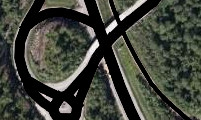
\includegraphics[width=\textwidth]{figs/illsuited_label2.jpg}
\caption{Road pixels superimposed.} \label{fig:ill-suited_example2}
\vspace{0.9cm} % separation vertically between the subfigures
\end{subfigure}

\caption[Examples of ill-suited line thickness]{Examples of ill-suited line thickness.} \label{fig:ill-suited}
\end{figure}



\chapter{Conclusion}
\label{cha:evaluationAndConclusion}
The goal of this thesis was to create a road detection system able to detect roads from aerial images. This was achieved by utilizing a convolutional neural network, and creating a dataset from available map data. This thesis has given a brief introduction to road extraction systems, and the related problem of label noise, often found in aerial image datasets. This chapter concludes this work, by first giving a brief overview of the thesis in Section \ref{sec:summaryOverview}. Then in Section \ref{sec:SummaryDiscussion}, the research goal and questions are tackled, with the results from Chapter \ref{cha:ResearchAndResults} as basis. Contributions made by this thesis are discussed in Section \ref{sec:Contributions}, and suggestions for future work are presented in Section \ref{sec:futureWork}.\\

\section{Overview}
\label{sec:summaryOverview}
In Chapter \ref{cha:TheoryAndBackground}, the thesis presented background theory, and related works. the components of a \ac{CNN}s was briefly explained, as well as curriculum learning and approaches for dealing with nosy labels. The related works, presented studies involving road detection systems, semantic segmentation, approaches for dealing with noisy labels, and curriculum learning. The issue of label noise in aerial imagery, have been influential in the choice of a curriculum strategy, and the studies have inspired the testing methodology used in Chapter \ref{cha:ResearchAndResults}.\\

Chapter \ref{cha:architectureAndModel}, presented a detailed description about the selected methods and the aerial image dataset. This included, a presentation of the default hyperparameters, the architecture, the optimization and regularization methods used by the \ac{CNN}. The chapter also described how the Norwegian Roads Dataset was constructed from aerial imagery and existing map data, and why this type of dataset is compelling to test the proposed methods on.\\

Experimental results from the proposed methods and the road detection system was presented in Chapter \ref{cha:ResearchAndResults}. First, the design of the experiments were described, and the basis for conducting them. Then, the specific details and parameters for each experiment were listed. Finally, the results were presented, and then discussed. The results showed that examples presented early in optimization, influence the final outcome of training, and that curriculum learning consistently performed better than the baseline. Furthermore, the chosen curriculum strategy worked well in practice. The bootstrapping experiments revealed that they do provide some robustness against omission and registration errors, but that the performance gain was minor. The qualitative analysis of the best performing road detection system, showed that a lot of the supposedly incorrect predictions, is actually a result of incorrect label maps.\\

\section{Results}
\label{sec:SummaryDiscussion}
\todo[inline]{Merits and limitations}


\section{Contributions}~\label{cont}
\label{sec:Contributions}
This thesis sought to test approaches for dealing with noisy labels in real-world datasets. This is an compelling inquiry in the field of machine learning, where the trend of using deep neural networks with a huge number of adjustable parameters, requires large training sets to generalize well. There is an abundance of existing data available online, which can be used for learning. Unfortunately, in many cases this data lacks accurate labels for supervised training. To manually label the data can be expensive, and very time consuming in many domains, such as transcribing speech for speech recognition, and tracing ground truth for semantic segmentation. Automatically generating datasets from existing data sources are a quick and economical solution, but can result in datasets with a lot of label noise.\\

The problem of label noise, was therefore tackled in this thesis by testing two different methods. Bootstrapping modifies the loss function, in order to reduce the impact of inconsistent labels. Curriculum learning modifies the training regime by sorting the training set into stages from ``easy" to ``hard" examples. The sorting mechanism, or curriculum strategy is based on measuring inconsistencies between labels and teacher predictions. Coincidentally, ``hard" examples often have inconsistent labelling, and are therefore more likely to be presented at a later stage of optimization if the dataset is organized according to this curriculum strategy. In effect, inconsistent examples are a less frequent occurrence in the first stage of the curriculum dataset.\\
 
The curriculum strategy can most likely be applied to tasks in other domains, since the example difficulty estimator $d(y,q)$ does not rely on any intrinsic features of image data. However, the effectiveness of this curriculum strategy has not been verified for other domains than road detection in aerial images.\\

The thesis found that bootstrapping did show some robustness towards label noise. The effect was however not of any statistical significance. Furthermore, the base network also performed surprising well for very high rates of omission noise.\\

Curriculum learning demonstrated consistently improved generalization accuracy in the experiments. The improved accuracy, was observed both for the Massachusetts Roads Dataset, as well as for the Norwegian Roads Dataset. The experiments also showed that only changing the example distribution of the first stage training set, affected the final outcome of the training procedure.\\



\section{Future Work}
\label{sec:futureWork}
This section presents future work, such as how to further verify the proposed curriculum strategy and bootstrapping loss function. In addition, this section will suggest further improvements of the road detection system.\\

The most compelling improvement of the road detection system is by incorporating \ac{CRF} or a post processing neural network, as described in Section \ref{sec:related_works}. This was tested by \cite{Kluckner_semantic_height} and \cite{Mnih_aerial_images_noisy}, and yielded accuracy improvements. These methods can also result in a smoother image segmentation. \\

To use the road predictions further in GIS applications, the binary prediction images should be converted into road centerline vectors. To do this, the prediction images have to be combined, and the resulting segmentation image must be cleaned. Methods from computer vision might be applicable for this work. For instance in \citep{Song_road_extraction_svm}, shape descriptions were extracted from the segmentation images, which can be used to measure density and shape index. Based on these values, shapes which have measurements not characteristic of roads can be removed by a threshold operation. In addition, morphological operations, such as thinning or skeletonization can be applied to reduce the segmented road regions down to one pixel thick lines.\\

Another potential improvement of the results is by finding better hyperparameters. For instance, the experiments testing the performance of the road detection system showed that the model capacity was initially constrained. Increasing the number of adjustable weights in the convolutional layers improved the precision and recall breakeven point substantially. Combining dropout with max-norm regularization instead of L2 weight decay could also be interesting, since this configuration achieved better test classification error in \citep{Srivastava_dropout}.\\

The bootstrapping methods did not improve performance significantly. This might be related to ill-suited parameters. Further testing of parameter configurations could be considered. In addition, the bootstrapping method could be tested with increasing levels of registration noise. The confident bootstrapping loss function could also be explored further. An interesting comparison of the bootstrapping methods, is mapping the relationship between a decreasing parameter $\beta$ and their resulting performances. Based on the few experiments conducted, it seems that confident bootstrapping might be less sensitive to decreasing the $\beta_{min}$ parameter.\\

There are also some unresolved questions regarding curriculum learning, and the proposed curriculum strategy. For instance, is it worth including examples with a very high difficulty estimate? How do the data cleansing approaches described in Section \ref{sec:BackgroundAndMotivation}, compare to curriculum learning? The thesis also does not properly determine how experienced a teacher classifier has to be in order to create an effective curriculum dataset. Further tests could illuminate the relationship between the teacher classifier's competency and the effectiveness of the curriculum strategy.  \\

The curriculum learning approach should also be tested on a network trained on a very large dataset. This could alternatively be tested by mapping the impact of curriculum learning for increasing training set sizes. The proposed strategy should also be compared to \ac{SPL} \citep{Kumar_self_paced_learning}, which internalizes the curriculum learning mechanism in its loss function.\\

Furthermore, \cite{Lu_self-paced_learning_diversity} illustrated the need for balancing diversity and easiness in curriculum learning. The \ac{SPL} approach is extended by a preference for both easy and diverse examples. This could potentially be done for the proposed curriculum strategy as well. For instance, unsupervised learning techniques, such as clustering, can organize the images into groups based on their similarity. The curriculum dataset can then be constructed with an equal representation of every cluster group. This might allow a reduction of the difficulty threshold $D_0$ without negatively impacting the performance.\\

The current version of the curriculum strategy was effective for two different datasets containing aerial imagery. However, the method should be tested for tasks in other domains as well. This might properly determine whether the proposed curriculum strategy can be generally applicable.\\
 



\backmatter


\appendix
\chapter*{Appendices}
\addcontentsline{toc}{chapter}{Appendices}
\renewcommand{\thesection}{\Alph{section}}
\section{System instructions}
\label{app:system_instructions}
In order to run the core system the following dependencies are required:
\begin{itemize}
\item Python 2.7
\item Theano
\item Numpy
\item Unirest
\item Python Imaging Library (PIL)
\end{itemize}

The system has only been tested with Ubuntu 14.04, but it should be possible to run on both Windows and Linux as long as the listed dependencies have been installed. Ubuntu is highly recommended because of a more convenient installation process. \\

A Nvidia GPU is also highly recommended for running the system. In most instances a GPU can give considerable speed improvements when training compared to a CPU. This is critical when having to deal with large datasets and models with millions of parameters. In order for Theano to efficiently use your GPU while training, CUDA Toolkit has to be installed. \\

A graphical user interface can also be utilized for monitoring the training. Running experiments can be stopped from this user interface, as well as a debugging option which display examples and model predictions. In addition all experiment data and results are stored as JSON, and can be viewed in the user interface. This includes, a loss per epoch plot, precision and recall curve and hyperparameters configuration. \\

The monitoring system can either be run locally, or installed on a server. All communication between the core system and the monitoring system is done by HTTP messaging. To enable monitoring, {\it enable\_gui} should be set to true in the core system's config file. Furthermore, the url to the monitoring system's api must also be set for the {\it endpoint} parameter. in  Utilizing this monitoring system requires these dependencies:
\begin{itemize}
\item Node.js
\item MongoDB
\end{itemize}

For installation instructions, see Appendix \ref{app:monitorInstall} and Appendix \ref{app:ubuntuInstall}. Alternatively, installation guides have been included in the README files of the repositories. The URL of these repositories are listed below:

\begin{itemize}
\item https://github.com/olavvatne/CNN
\item https://github.com/olavvatne/ml-monitor
\end{itemize} 


\section{System Installation Guide - Ubuntu}
\label{app:ubuntuInstall}
This guide will help you install all dependencies required for running Theano with a GPU, which should be done in order to run the system. \\
\noindent Install all dependencies:
\begin{lstlisting}[language=bash]
  $ sudo apt-get install -y gcc g++ gfortran build-essential git
   wget linux-image-generic libopenblas-dev python-dev python-pip 
   python-nose python-numpy python-scipy  
\end{lstlisting}
~\\

\noindent Install Theano:
\begin{lstlisting}[language=bash]
  $ sudo pip install --upgrade --no-deps 
  git+git://github.com/Theano/Theano.git
\end{lstlisting}
~\\

\noindent Download Cuda 7 toolkit:
\begin{lstlisting}[language=bash]
  $ sudo wget http://developer.download.nvidia.com/
  compute/cuda/repos/ubuntu1404/x86_64/
  cuda-repo-ubuntu1404_7.0-28_amd64.deb
\end{lstlisting}
~\\

\noindent Depackage Cuda:
\begin{lstlisting}[language=bash]
  $ sudo dpkg -i cuda-repo-ubuntu1404_7.0-28_amd64.deb  
\end{lstlisting}
~\\

\noindent Install the cuda driver:
\begin{lstlisting}[language=bash]
  $ sudo apt-get update
  $ sudo apt-get install -y cuda  
\end{lstlisting}
~\\

\noindent Append path for Cuda nvcc in PATH and add LD\_LIBRARY\_PATH in the .bashrc file (see Table \ref{tab:install_bash_paths}). Then do a reboot:

\FloatBarrier
\begin{table}[!htbp]
\caption[Paths to include]{Paths to include.}
\begin{center}
\begin{adjustbox}{max width=\textwidth}
\begin{tabular}{ l }
  \hline			
  export PATH=(...):/usr/local/cuda/bin  \\
  export LD\_LIBRARY\_PATH=/usr/local/cuda/lib64 \\
  \hline  
\end{tabular}
\end{adjustbox}
\end{center}
\label{tab:install_bash_paths}
\end{table}
\FloatBarrier

\noindent  Create a theano config file as illustrated in Table \ref{tab:install_theano_config_file}. Name this file .theanorc and place it in your home directory:\\

\FloatBarrier
\begin{table}[!htbp]
\caption[Theano config file]{Theano config file.}
\begin{center}
\begin{adjustbox}{max width=\textwidth}
\begin{tabular}{ l }
  \hline			
  ~[global] \\
  floatX=float32 \\
  device=gpu \\
  mode=FAST\_RUN \\
  \\
  ~[nvcc] \\
  fastmath=True \\
  \\
  ~[cuda] \\
  root=/usr/local/cuda \\
  \hline  
\end{tabular}
\end{adjustbox}
\end{center}
\label{tab:install_theano_config_file}
\end{table}
\FloatBarrier

\noindent Clone CNN repository, which contains the core system:
\begin{lstlisting}[language=bash]
  $ git clone https://github.com/olavvatne/CNN.git 
\end{lstlisting}
~\\

\noindent Navigate to the root of the cloned repository. Create a secret.py file, and put the token created for the Monitoring Interface in a variable. See Appendix \ref{app:monitorInstall}:
\begin{lstlisting}[language=bash]
  token = "Bearer " + ml-monitor-token
\end{lstlisting}
~\\

\section{Monitoring Interface Installation Guide - Ubuntu}
\label{app:monitorInstall}
This guide outlines the steps required for setting up the monitoring interface. This guide can also be found in the repository's README file. Some of the steps are slightly different for Windows. \\

\noindent Clone the ml-monitor repository:
\begin{lstlisting}[language=bash]
  $ git clone https://github.com/olavvatne/ml-monitor.git
\end{lstlisting}
~\\

\noindent Install Node.js on your system:
\begin{lstlisting}[language=Python]
  $ sudo apt-get update
  $ sudo apt-get install nodejs
\end{lstlisting}
~\\

\noindent Install npm package manager:
\begin{lstlisting}[language=bash]
    Install npm package manager:
\end{lstlisting}
~\\

\noindent Install MongoDB:
\noindent Navigate to ml-monitor, and install the dependencies of ml-monitor:
\begin{lstlisting}[language=bash]
    $ npm install
\end{lstlisting}
~\\

\noindent Before running ml-monitor, some database collections and a user have to be created in Mongo Shell:
\begin{lstlisting}[language=bash]
    $ export LC_ALL=C (Optional. Might be necessary)
    $ mongo
\end{lstlisting}
~\\

\noindent Inside Mongo Shell, first create a new database:
\begin{lstlisting}[language=bash]
    > use ml-monitor
\end{lstlisting}
~\\

\noindent Then create the database collections required by ml-monitor:
\begin{lstlisting}[language=bash]
    > db.createCollection('experimentlist')
    > db.createCollection('userlist')
    > db.createCollection('grouplist')
\end{lstlisting}
~\\

\noindent Create a user. The authentication system is very simple, so remember to create a long random string of characters as token:
\begin{lstlisting}[language=bash]> 
    db.userlist.insert(
    {"user": "ola", "password": "password", "token": "String"})
\end{lstlisting}
~\\

\noindent Finally, insert the default group, that new experiments will be assigned to:
\begin{lstlisting}[language=bash]
    > db.grouplist.insert(
    {"name": "unassigned", "gid": "0", "date_created": new Date()})
\end{lstlisting}
~\\

\noindent To start the system, run:
\begin{lstlisting}[language=bash]
    $ npm run start
\end{lstlisting}

\section{Experiment tools overview}
\label{app:tools}
All tools which have been created for this thesis are listed below. The source code can be found inside the tools module of the road detection system's repository.
\begin{itemize}
\item measurement.precisionrecall.py\\
The tool creates the precision and recall curve. Command line options can be supplied.
\item layer.visualize.py\\
Opens a params.pkl file, containing the weights and hyperparameter configuration of a trained network. It creates a visualization of the kernels in the network's input layer.
\item distribution.curriculum\_diff.py\\
Samples patch examples and creates a histogram showing the patch dataset difficulty estimate distribution. Useful for setting the  threshold $D_\theta$ when conducting experiments. Also useful for verifying the content in a curriculum patch dataset stage.
\item distribution.dataset\_std.py\\
Tool for finding an estimate of a dataset's standard deviation. This value is used by the contrast normalization in the pre-processing step.
\item distribution.label\_dist\\
Counts the percentage of true label pixels in a dataset with binary labels.
\item curriculum.dataset\_create.py\\
Tool for pre-generating a curriculum patch dataset. Command line options can be supplied to, select a teacher, the thresholds $D_\theta$, the teacher's optimal threshold value, and dataset. The tool also comes with a baseline option which generate a staged patch dataset without curating the content of each stage.
\item convert.alpha.py\\
Converts a RGB dataset to RGBA. A quirk of the Python module PIL makes RGBA preferable when rotating an images. Areas not covered by pixels after a rotation, aare set to transparent with RGBA. With RGB, these pixels are set to black, which results in a lot of patch examples with no content.
\item figure.average\_compare.py\\
Averages experiment runs, and plots the averaged MSE loss and precision and recall curve from the test dataset. The tool also marks the precision and recall breakeven point for each plot. The resulting figures are used for comparison purposes in this thesis.
\item figure.average\_loss.py\\
Averages the test, validation and training loss from experiment replicates, and plots the result in a loss per epoch plot. 
\item figure.average\_noise\_levels\\
Averages the final epoch's test loss of an experiment. It also averages the precision and recall breakeven of each replicate experiment. The figures created by this tools, show the MSE loss and breakeven point, over increasing levels of label noise.
\end{itemize}

\section{Experiment Population Normality Assumption}
\label{app:normality}
The Welch's t test assumes that the samples are independent, and drawn from an approximately normal distributed population. In this appendix, the assumption of normality is explored further.\\

One way of verifying that a population do not violate the normality assumption is to create a normal Q-Q plot. These plots plot each sample based on its quantile and the corresponding theoretical quantile expected from a normal distribution. The population samples are normally distributed if the plotted points approximately fit a 45 degree line. The normal Q-Q plots comparing the test loss populations of {\it Experiment E1 - 0\% omission noise} to normal distributions can be found in Figure \ref{fig:normality_baseline} and Figure \ref{fig:normality_bootstrapping}. The plots are clearly affected by sample variability caused by the small sample sizes. This can be seen in Figure \ref{fig:normality_random}, where samples randomly picked from a normal distribution are plotted.  This plot is created from 10 randomly drawn samples of a normal distribution with mean and variance equal to that of the baseline population. Figure \ref{fig:normality_random100} displays the normal Q-Q plot of 100 random samples drawn from a normal distribution. This plot fits the line more closely than \ref{fig:normality_random}. Because of the small sample sizes, it can be hard to confidently assess whether the experiment populations are normally distributed or not.  \\

\begin{figure}
\begin{subfigure}{0.38\textwidth}
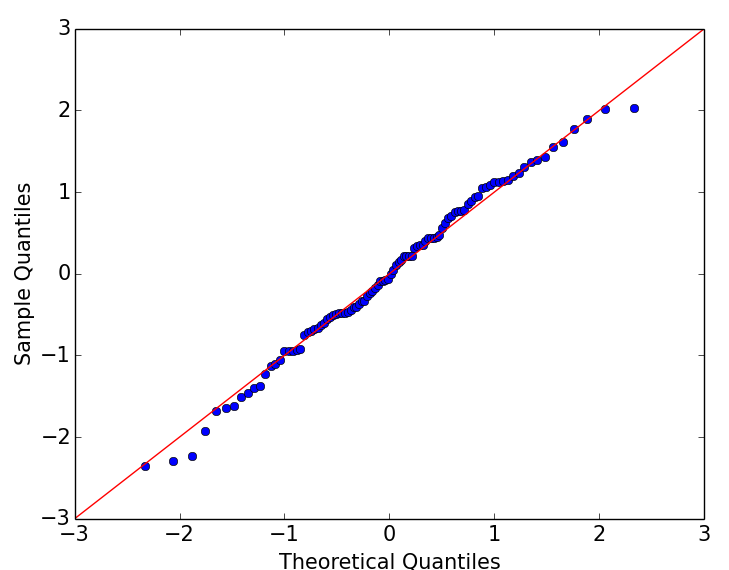
\includegraphics[width=\linewidth]{figs/normality/100samples_random2.png}
\caption{100 samples from a normal distribution} \label{fig:normality_random100}
\end{subfigure}
\hspace*{\fill} % separation between the subfigures
\begin{subfigure}{0.38\textwidth}
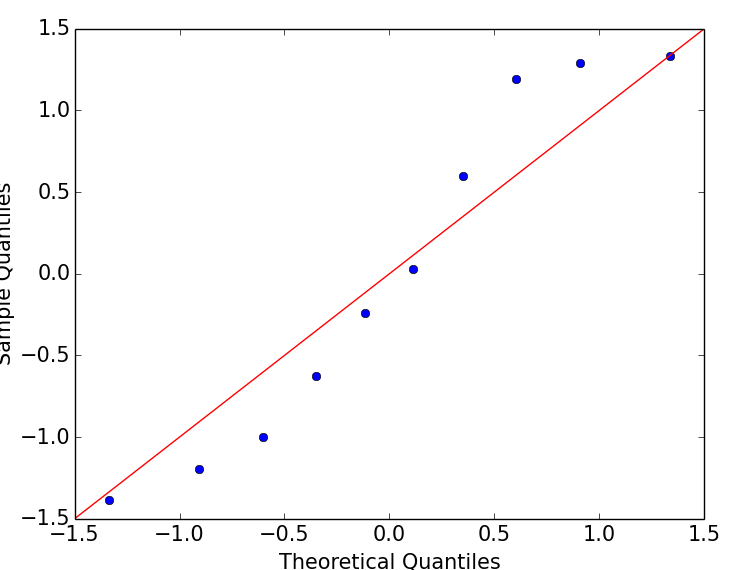
\includegraphics[width=\linewidth]{figs/normality/10samples_random2.png}
\caption{10 samples from a normal distribution} \label{fig:normality_random}
\end{subfigure}

\begin{subfigure}{0.38\textwidth}
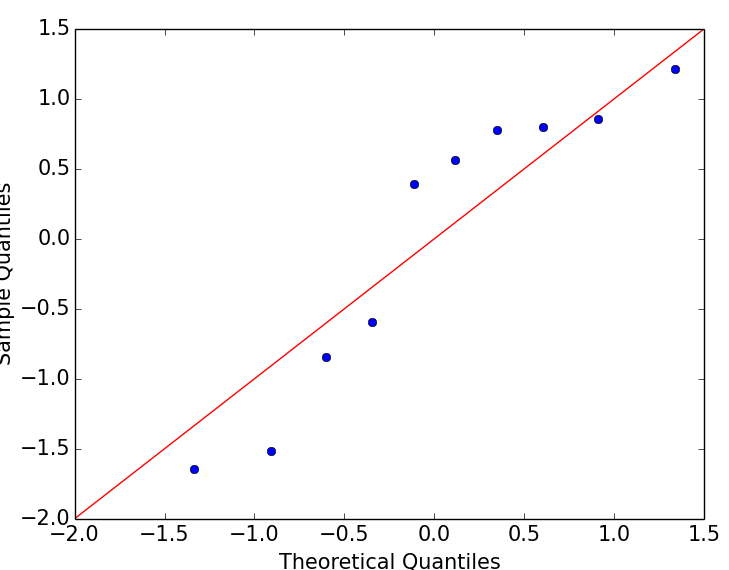
\includegraphics[width=\linewidth]{figs/normality/10samples_baseline2.png}
\caption{Baseline samples from Experiment E1} \label{fig:normality_baseline}
\end{subfigure}
\hspace*{\fill} % separation between the subfigures
\begin{subfigure}{0.38\textwidth}
\includegraphics[width=\linewidth]{figs/normality/10samples_bootstrapping2.png}
\caption{Bootstrapping samples from Experiment E1} \label{fig:normality_bootstrapping}
\end{subfigure}
\caption[Normal Q-Q plot example]{Normal Q-Q plots generated by samples from a normal distribution, and from the baseline and curriculum population of Experiment E1 - 0\% omission noise. } \label{fig:normalityqq}
\end{figure}


\section{Increasing Levels of Random Noise Experiment}
\label{app:randomnoiseexperiment}
\todo[inline]{Do this}
\todo[inline]{Test loss figure for bootstrapping and baseline (confident if time allows}
\todo[inline]{Explain results.}
\todo[inline]{Noise illustration, random noise vs omission noise}

\pagebreak
\section{Road Detection Systems Results}
\label{app:roaddetectionresults}
In this appendix results from the best performing convolutional neural networks are displayed. The precision and recall breakeven point of the model trained on the Massachusetts Roads Dataset is 0.8627. Whereas, the breakeven point for the best model trained on the Norwegian Roads Dataset is 0.7620.

\begin{figure}[H]
\begin{subfigure}{0.23\textwidth}
\includegraphics[width=\textwidth]{figs/appendix/img1151.jpg}
\caption{ Image. }
\vspace{0.1cm} % separation vertically between the subfigures
\end{subfigure}
\hspace*{\fill} % separation between the subfigures
\begin{subfigure}{0.23\textwidth}
\includegraphics[width=\textwidth]{figs/appendix/label1151.jpg}
\caption{ Label. }
\vspace{0.1cm} % separation vertically between the subfigures
\end{subfigure}
\hspace*{\fill} % separation between the subfigures
\begin{subfigure}{0.23\textwidth}
\includegraphics[width=\textwidth]{figs/appendix/pred1151.jpg}
\caption{ Prediction. }
\vspace{0.1cm} % separation vertically between the subfigures
\end{subfigure}
\hspace*{\fill} % separation between the subfigures
\begin{subfigure}{0.23\textwidth}
\includegraphics[width=\textwidth]{figs/appendix/hit1151.jpg}
\caption{ Hits. }
\vspace{0.1cm} % separation vertically between the subfigures
\end{subfigure}
\begin{subfigure}{0.23\textwidth}
\includegraphics[width=\textwidth]{figs/appendix/img1160.jpg}
\caption{ Image.}
\vspace{0.1cm} % separation vertically between the subfigures
\end{subfigure}
\hspace*{\fill} % separation between the subfigures
\begin{subfigure}{0.23\textwidth}
\includegraphics[width=\textwidth]{figs/appendix/label1160.jpg}
\caption{Label}
\vspace{0.1cm} % separation vertically between the subfigures
\end{subfigure}
\hspace*{\fill} % separation between the subfigures
\begin{subfigure}{0.23\textwidth}
\includegraphics[width=\textwidth]{figs/appendix/pred1160.jpg}
\caption{Prediction.}
\vspace{0.1cm} % separation vertically between the subfigures
\end{subfigure}
\hspace*{\fill} % separation between the subfigures
\begin{subfigure}{0.23\textwidth}
\includegraphics[width=\textwidth]{figs/appendix/hit1160.jpg}
\caption{Hits.}
\vspace{0.1cm} % separation vertically between the subfigures
\end{subfigure}
\begin{subfigure}{0.23\textwidth}
\includegraphics[width=\textwidth]{figs/appendix/img1205.jpg}
\caption{ Image. }
\vspace{0.1cm} % separation vertically between the subfigures
\end{subfigure}
\hspace*{\fill} % separation between the subfigures
\begin{subfigure}{0.23\textwidth}
\includegraphics[width=\textwidth]{figs/appendix/label1205.jpg}
\caption{ Label. }
\vspace{0.1cm} % separation vertically between the subfigures
\end{subfigure}
\hspace*{\fill} % separation between the subfigures
\begin{subfigure}{0.23\textwidth}
\includegraphics[width=\textwidth]{figs/appendix/pred1205.jpg}
\caption{ Prediction. }
\vspace{0.1cm} % separation vertically between the subfigures
\end{subfigure}
\hspace*{\fill} % separation between the subfigures
\begin{subfigure}{0.23\textwidth}
\includegraphics[width=\textwidth]{figs/appendix/hit1205.jpg}
\caption{ Hits. }
\vspace{0.1cm} % separation vertically between the subfigures
\end{subfigure}
\begin{subfigure}{0.23\textwidth}
\includegraphics[width=\textwidth]{figs/appendix/img1217.jpg}
\caption{ Image.}
\vspace{0.1cm} % separation vertically between the subfigures
\end{subfigure}
\hspace*{\fill} % separation between the subfigures
\begin{subfigure}{0.23\textwidth}
\includegraphics[width=\textwidth]{figs/appendix/label1217.jpg}
\caption{Label}
\vspace{0.1cm} % separation vertically between the subfigures
\end{subfigure}
\hspace*{\fill} % separation between the subfigures
\begin{subfigure}{0.23\textwidth}
\includegraphics[width=\textwidth]{figs/appendix/pred1217.jpg}
\caption{Prediction.}
\vspace{0.1cm} % separation vertically between the subfigures
\end{subfigure}
\hspace*{\fill} % separation between the subfigures
\begin{subfigure}{0.23\textwidth}
\includegraphics[width=\textwidth]{figs/appendix/hit1217.jpg}
\caption{Hits.}
\vspace{0.1cm} % separation vertically between the subfigures
\end{subfigure}
\vspace{-1\baselineskip}
\caption[Norway Road extraction results]{Road extraction results from the Norwegian Roads Dataset.} \label{fig:Norway_app_results2}
\end{figure}

\begin{figure}[H]
\begin{subfigure}{0.23\textwidth}
\includegraphics[width=\textwidth]{figs/appendix/img11128870_15.jpg}
\caption{ Image. }
\vspace{0.2cm} % separation vertically between the subfigures
\end{subfigure}
\hspace*{\fill} % separation between the subfigures
\begin{subfigure}{0.23\textwidth}
\includegraphics[width=\textwidth]{figs/appendix/label11128870_15.jpg}
\caption{ Label. }
\vspace{0.2cm} % separation vertically between the subfigures
\end{subfigure}
\hspace*{\fill} % separation between the subfigures
\begin{subfigure}{0.23\textwidth}
\includegraphics[width=\textwidth]{figs/appendix/pred11128870_15.jpg}
\caption{ Prediction. }
\vspace{0.2cm} % separation vertically between the subfigures
\end{subfigure}
\hspace*{\fill} % separation between the subfigures
\begin{subfigure}{0.23\textwidth}
\includegraphics[width=\textwidth]{figs/appendix/hit11128870_15.jpg}
\caption{ Hits. }
\vspace{0.2cm} % separation vertically between the subfigures
\end{subfigure}
\begin{subfigure}{0.23\textwidth}
\includegraphics[width=\textwidth]{figs/appendix/img11728825_15.jpg}
\caption{ Image.}
\vspace{0.2cm} % separation vertically between the subfigures
\end{subfigure}
\hspace*{\fill} % separation between the subfigures
\begin{subfigure}{0.23\textwidth}
\includegraphics[width=\textwidth]{figs/appendix/label11728825_15.jpg}
\caption{Label}
\vspace{0.2cm} % separation vertically between the subfigures
\end{subfigure}
\hspace*{\fill} % separation between the subfigures
\begin{subfigure}{0.23\textwidth}
\includegraphics[width=\textwidth]{figs/appendix/pred11728825_15.jpg}
\caption{Prediction.}
\vspace{0.2cm} % separation vertically between the subfigures
\end{subfigure}
\hspace*{\fill} % separation between the subfigures
\begin{subfigure}{0.23\textwidth}
\includegraphics[width=\textwidth]{figs/appendix/hit11728825_15.jpg}
\caption{Hits.}
\vspace{0.2cm} % separation vertically between the subfigures
\end{subfigure}
\begin{subfigure}{0.23\textwidth}
\includegraphics[width=\textwidth]{figs/appendix/img20878930_15.jpg}
\caption{ Image. }
\vspace{0.2cm} % separation vertically between the subfigures
\end{subfigure}
\hspace*{\fill} % separation between the subfigures
\begin{subfigure}{0.23\textwidth}
\includegraphics[width=\textwidth]{figs/appendix/label20878930_15.jpg}
\caption{ Label. }
\vspace{0.2cm} % separation vertically between the subfigures
\end{subfigure}
\hspace*{\fill} % separation between the subfigures
\begin{subfigure}{0.23\textwidth}
\includegraphics[width=\textwidth]{figs/appendix/pred20878930_15.jpg}
\caption{ Prediction. }
\vspace{0.2cm} % separation vertically between the subfigures
\end{subfigure}
\hspace*{\fill} % separation between the subfigures
\begin{subfigure}{0.23\textwidth}
\includegraphics[width=\textwidth]{figs/appendix/hit20878930_15.jpg}
\caption{ Hits. }
\vspace{0.2cm} % separation vertically between the subfigures
\end{subfigure}
\begin{subfigure}{0.23\textwidth}
\includegraphics[width=\textwidth]{figs/appendix/img24628885_15.jpg}
\caption{ Image.}
\vspace{0.2cm} % separation vertically between the subfigures
\end{subfigure}
\hspace*{\fill} % separation between the subfigures
\begin{subfigure}{0.23\textwidth}
\includegraphics[width=\textwidth]{figs/appendix/label24628885_15.jpg}
\caption{Label}
\vspace{0.2cm} % separation vertically between the subfigures
\end{subfigure}
\hspace*{\fill} % separation between the subfigures
\begin{subfigure}{0.23\textwidth}
\includegraphics[width=\textwidth]{figs/appendix/pred24628885_15.jpg}
\caption{Prediction.}
\vspace{0.2cm} % separation vertically between the subfigures
\end{subfigure}
\hspace*{\fill} % separation between the subfigures
\begin{subfigure}{0.23\textwidth}
\includegraphics[width=\textwidth]{figs/appendix/hit24628885_15.jpg}
\caption{Hits.}
\vspace{0.2cm} % separation vertically between the subfigures
\end{subfigure}
\vspace{-1\baselineskip}
\caption[Massachusetts Road extraction results]{Road extraction results from the Massachusetts Roads Dataset.} \label{fiMass_app_results2}
\end{figure}

\pagebreak
\section{Experiment E2 Results}
\label{app:fullE5results}
The results from Experiment E2 were summarised by plotting the final test loss and precision and breakeven point for increasing levels of omission noise. In this appendix, the test loss figures for every noise rate is shown in Figure \ref{fig:E2_all_lc}, while the precision and recall curve figures are depicted in Figure \ref{fig:E2_all_pr}.
\begin{figure}[H]
\begin{subfigure}{0.31\textwidth}
\includegraphics[width=\textwidth]{figs/E2/pr_0.png}
\caption{ 0\% } \label{fig:app_E2_0_pr}
\vspace{-0.1cm} % separation vertically between the subfigures
\end{subfigure}
\hspace*{\fill} % separation between the subfigures
\begin{subfigure}{0.31\textwidth}
\includegraphics[width=\textwidth]{figs/E2/pr_1.png}
\caption{10\% } \label{fig:app_E2_1_pr}
\vspace{-0.1cm} % separation vertically between the subfigures
\end{subfigure}
\hspace*{\fill} % separation between the subfigures
\begin{subfigure}{0.31\textwidth}
\includegraphics[width=\textwidth]{figs/E2/pr_2.png}
\caption{20\% } \label{fig:app_E2_2_pr}
\vspace{-0.1cm} % separation vertically between the subfigures
\end{subfigure}
\begin{subfigure}{0.31\textwidth}
\includegraphics[width=\textwidth]{figs/E2/pr_3.png}
\caption{ 30\%} \label{fig:app_E2_3_pr}
\vspace{-0.1cm} % separation vertically between the subfigures
\end{subfigure}
\hspace*{\fill} % separation between the subfigures
\begin{subfigure}{0.31\textwidth}
\includegraphics[width=\textwidth]{figs/E2/pr_4.png}
\caption{40\%} \label{fig:app_E2_4_pr}
\vspace{-0.1cm} % separation vertically between the subfigures
\end{subfigure}
\vspace{-0.6\baselineskip}
\caption{E2 - Precision and recall plot for several levels of omission noise.} \label{fig:E2_all_pr}
\end{figure}
\vspace{-0.7cm}
\begin{figure}[H]
\begin{subfigure}{0.3\textwidth}
\includegraphics[width=\textwidth]{figs/E2/lc_0.png}
\caption{ 0\% } \label{fig:app_E2_0_lc}
\vspace{-0.1cm} % separation vertically between the subfigures
\end{subfigure}
\hspace*{\fill} % separation between the subfigures
\begin{subfigure}{0.31\textwidth}
\includegraphics[width=\textwidth]{figs/E2/lc_1.png}
\caption{10\% } \label{fig:app_E2_1_lc}
\vspace{-0.1cm} % separation vertically between the subfigures
\end{subfigure}
\hspace*{\fill} % separation between the subfigures
\begin{subfigure}{0.31\textwidth}
\includegraphics[width=\textwidth]{figs/E2/lc_2.png}
\caption{20\% } \label{fig:app_E2_2_lc}
\vspace{-0.1cm} % separation vertically between the subfigures
\end{subfigure}
\begin{subfigure}{0.31\textwidth}
\includegraphics[width=\textwidth]{figs/E2/lc_3.png}
\caption{ 30\%} \label{fig:app_E2_3_lc}
\vspace{-0.1cm} % separation vertically between the subfigures
\end{subfigure}
\hspace*{\fill} % separation between the subfigures
\begin{subfigure}{0.31\textwidth}
\includegraphics[width=\textwidth]{figs/E2/lc_4.png}
\caption{40\%} \label{fig:app_E2_4_lc}
\vspace{-0.1cm} % separation vertically between the subfigures
\end{subfigure}
\vspace{-0.6\baselineskip}
\caption{E2 - Test loss comparisons for several levels of omission noise.} \label{fig:E2_all_lc}
\end{figure}


\section{TODOs which apply to entire thesis}
\todo[inline]{Remove this part!}
\begin{itemize}
\item proof read (second time, and be vary of incorrect tense. Also look out for long sentences, and tedious language. If used is used to often, make some fixes here as well)
\item Ensure either by a footnote or something that road extraction and road detection and so forth is the same thing
\item What does harder examples look like? Examples
\item Example of road removal first paragraph Section 4.3.1, Maybe in appendix?
\item organize with s because of british english?
\item Appendix for other results? Random noise results? 

\item Road extraction, road detection, semantic segmentation, patch-based. That they are the same thing needs to be integrated somewhere
\item Check that installation guides, or should they be removed because of length. They are in repositories so.. and dependencies are correct - Appendix A, B, C
\end{itemize}


\addcontentsline{toc}{chapter}{Bibliography}
\bibliography{./bibtex/bibliography}

%\chapter{Appendices}
%\label{cha:appendices}
%\listoftodos
\end{document}
